\documentclass[10pt]{beamer}

\usetheme{Antibes}
\usecolortheme{orchid}

\useinnertheme{rectangles} 
\useoutertheme{infolines}   
\setbeamertemplate{navigation symbols}{} 

\usepackage[spanish]{babel}
\usepackage{booktabs}
\usepackage[sfdefault]{FiraSans} 
\usepackage[utf8]{inputenc}
\usepackage{siunitx}
\usepackage{tikz}
\usepackage{threeparttable}


\title[Consumo Energético en una BD Dist.]{
  Evaluación Empírica Del Consumo Energético Y Rendimiento En Una Base De Datos
  Distribuida
}
\subtitle{Proyecto de grado a dedicación exclusiva}
\author[Márquez, F. \& Goncalves, M.]{
  Lic. Francisco Márquez\\ \and \footnotesize{Asesoría: Dr. Marlene Goncalves}
}
\institute[USB]{
  Universidad Simón Bolívar \\
  Decanato de Estudios Profesionales \\
  Coordinación de Ingeniería de Computación
}
\date[Julio 2026]{Julio de 2026}

\AtBeginSection[]{
  \begin{frame}{Contenido}
    \tableofcontents[currentsection]
  \end{frame}
}

\addto\captionsspanish{
  \renewcommand{\tablename}{Tabla}
}

\usetikzlibrary{er}
\tikzset{multi attribute/.style={attribute,double distance=1.5pt}}
\tikzset{derived attribute/.style={attribute,dashed}}
\tikzset{total/.style={double distance=1.5pt}}
\tikzset{every entity/.style={draw=orange,fill=orange!20}}
\tikzset{every attribute/.style={draw=red,fill=red!20}}
\tikzset{every relationship/.style={draw=blue,fill=blue!20}}

\DeclareUnicodeCharacter{2705}{$\checkmark$}

\setbeamertemplate{bibliography item}{\insertbiblabel}

\begin{document}
  \begin{frame}
    \titlepage
  \end{frame}

  \begin{frame}{Contenido}
    \tableofcontents
  \end{frame}

  \section{El problema} % (fold)
  \label{sec:el_problema}
    \begin{frame}{El Problema}
      \begin{table}
        \caption{Estado del arte}
        \footnotesize
        \begin{tabular}{| c c c c c c |}
          \hline
                    Referencia         & BD distribuida & BD Relacional & TPC-H & Diseño físico & Escalabilidad \\ \hline
          \cite{bunseenergy2014}       &       ✅       &               &       &               &               \\ \hline
          \cite{xuexploring2010}       &       ✅       &       ✅      &  ✅   &               &       ✅      \\ \hline
          \cite{langtowards2009}       &                &       ✅      &  ✅   &               &               \\ \hline
          \cite{langrethinking2011}    &                &               &  ✅   &               &               \\ \hline
          \cite{langtowards2012}       &                &       ✅      &  ✅   &               &       ✅      \\ \hline
          \cite{niemanndoes2013}       &                &       ✅      &  ✅   &               &       ✅      \\ \hline
          \cite{niemannevaluating2013} &                &       ✅      &  ✅   &               &       ✅      \\ \hline
          \cite{duarteevaluating2018}  &       ✅       &               &       &               &               \\ \hline
          \cite{shahcomprehensive2022} &       ✅       &               &       &               &               \\ \hline
          \cite{foschinisql2023}       &       ✅       &       ✅      &       &       ✅      &       ✅      \\ \hline
          \cite{gomesenergy2016}       &       ✅       &               &       &               &               \\ \hline
          \cite{gomesnosql-based2023}  &       ✅       &               &       &               &               \\ \hline
          \cite{guoenergy2024}         &       ✅       &       ✅      &  ✅   &               &               \\ \hline
          \cite{subramaniamenergy2015} &       ✅       &               &       &               &               \\ \hline
          \cite{niemanntowards2016}    &       ✅       &               &       &               &               \\ \hline
          \cite{roukhenergy-aware2016} &                &       ✅      &  ✅   &               &               \\ \hline
        \end{tabular}
      \end{table}
    \end{frame}

    \begin{frame}{Objetivos}
      \begin{exampleblock}{Objetivo General}
      Comparar el rendimiento y el consumo energético en un ambiente
      distribuido, con y sin diseño físico, utilizando el \textit{benchmark}
      TPC-H y el sistema de bases de datos PostgreSQL.
      \end{exampleblock}

      \vspace{0.4cm}

      \begin{block}{Objetivos Específicos}
        \only<1-2>{
          \begin{enumerate}
            \item<1-> Determinar el comportamiento del rendimiento y el consumo
            energético en el sistema de bases de datos PostgreSQL mediante las
            pruebas de rendimiento TPC-H en un ambiente distribuido sin diseño
            físico a varios volúmenes de datos.
            \item<2-> Caracterizar los parámetros de rendimiento y el consumo
            energético en el sistema gestor de bases de datos PostgreSQL
            mediante las pruebas de rendimiento TPC-H en un ambiente distribuido
            con diseño físico a varios volúmenes de datos.
          \end{enumerate}
        }
        \only<3-4>{
          \renewcommand{\insertenumlabel}{\the\numexpr\value{enumi}+2\relax}
          \begin{enumerate}
            \item<3-> Comparar el comportamiento del sistema gestor de bases
            de datos PostgreSQL en términos de rendimiento y consumo energético
            bajo las pruebas de rendimiento TPC-H en un ambiente distribuido con
            y sin diseño físico.
            \item<4-> Evaluar el impacto de la estrategia de diseño físico
            aplicada sobre el sistema gestor de bases de datos PostgreSQL
            mediante las pruebas de rendimiento TPC-H en un ambiente
            distribuido.
          \end{enumerate}
        }
      \end{block}
    \end{frame}
  % section el_problema (end)

  \section{Marco teórico} % (fold)
  \label{sec:marco_teórico}
    \begin{frame}{El \textit{benchmark} TPC-H}
      \begin{figure}[H]
        \centering
        \begin{tikzpicture}[node distance=5em]
          \node[entity] (r) {REGION};
          \node[relationship] (bto) [left of=r]{\tiny Belongs to} edge (r);
          \node[entity] (n) [below of=bto] {NATION} edge (bto);
          \node[relationship] (ctzn) [right of=n] {\tiny is} edge (n);
          \node[entity] (cust) [right of=ctzn] {CUSTOMER} edge (ctzn);
          \node[relationship] (plcs)[below of=cust]{\tiny Places}edge(cust);
          \node[entity] (o) [below of=plcs] {ORDERS} edge (plcs);
          \node[relationship] (cons) [left of=o]{\tiny Constitutes}edge (o);
          \node[entity] (l) [left of=cons] {LINEITEM} edge (cons);
          \node[relationship] (sto) [left of=n] {\tiny Supplies to}edge (n);
          \node[entity] (supp) [below of=sto] {SUPPLIER} edge (sto);
          \node[relationship] (psup) [left of=l] {\tiny Partsupp} edge (l)
                                                                  edge (supp);
          \node[entity] (part) [left of=psup] {PART} edge (psup);
        \end{tikzpicture}
        \caption{Diagrama Entidad Relación simplificado sin atributos}
      \end{figure}
    \end{frame}

    \begin{frame}{Diseño lógico}
      \footnotesize
      \begin{itemize}
        \item \texttt{Region(\underline{regionkey}, name, comment)}
        \item \texttt{Nation(\underline{nationkey}, name, $\overset{
          \texttt{region}}{\overline{\texttt{regionkey}}}$, comment)}
        \item \texttt{Part(\underline{partkey}, name, mfgr, brand, type, size,
        container, retailprice, comment)}
        \item \texttt{Customer(\underline{custkey}, name, address,
        $\overset{\texttt{nation}}{\overline{\texttt{nationkey}}}$, phone,
        acctbal, mktsegment, comment)}
        \item \texttt{Supplier(\underline{suppkey}, name, address,
        $\overset{\texttt{nation}}{\overline{\texttt{nationkey}}}$, phone,
        acctbal, comment)}          \item \texttt{Orders(\underline{orderkey},
        $\overset{\texttt{customer}}{\overline{\texttt{custkey}}}$,
        orderstatus, totalprice, orderpriority, clerk, shippriority, comment)}
        \item \texttt{Lineitem(\underline{$\overset{\texttt{orders}}{
          \overline{\texttt{orderkey}}}$, linenumber}, $\overset{\texttt{
          partsupp}}{\overline{\texttt{partkey},\ \texttt{supplier}}}$,
          quantity, extendedprice, discount, tax, returnflag, linestatus,
          shipdate, commitdate, receiptdate, shipinstruct, shipmode, comment)}
        \item \texttt{Partsupp(\underline{$\overset{\texttt{part}}{
          \overline{\texttt{partkey}}}$, $\overset{\texttt{supplier}}{
          \overline{\texttt{suppkey}}}$}, availqty, supplycost, comment)}
      \end{itemize}
    \end{frame}

    \begin{frame}{Consultas}
      \tiny
      \begin{table}[H]
        \centering
        \begin{threeparttable}
        \caption{Resumen de las implementaciones de las consultas}
        \begin{tabular}{| c | c | c | c | c | c |}
          \hline
          Consulta        & \texttt{JOIN} totales & Agregación & Niveles de anidamiento & Operaciones & Agrupamientos \\ \hline
              Q1          &           0           &      8     &            0           &       S     &       2       \\ \hline
              Q2          &         4 + 3         &      1     &            1           &       S     &       0       \\ \hline
              Q3          &           2           &      1     &            0           &       S     &       3       \\ \hline
              Q4          &         $1^b$         &      1     &            1           &       S     &       1       \\ \hline
              Q5          &           5           &      1     &            0           &       S     &       1       \\ \hline
              Q6          &           0           &      1     &            0           &       S     &       0       \\ \hline
              Q7          &           5           &      1     &            1           &       S     &       3       \\ \hline
              Q8          &           7           &      2     &            1           &       S     &       1       \\ \hline
              Q9          &           5           &      1     &            1           &       S     &       2       \\ \hline
             Q10          &           3           &      1     &            0           &       S     &       7       \\ \hline
             Q11          &         2 + 2         &      3     &            1           &       S     &       1       \\ \hline
             Q12          &           1           &      2     &            0           &       S     &       1       \\ \hline
             Q13\tnote{a} &         $1^c$         &      2     &            1           &       S     &       2       \\ \hline
             Q14          &           1           &      2     &            0           &       S     &       0       \\ \hline
             Q15          &           1           &      2     &            1           &      CSD    &       1       \\ \hline
             Q16\tnote{a} &       $1 + 1^d$       &      1     &            1           &       S     &       3       \\ \hline
             Q17          &       $1 + 1^b$       &      2     &            1           &       S     &       0       \\ \hline
             Q18          &       $2 + 1^b$       &      2     &            1           &       S     &       5       \\ \hline
             Q19          &           1           &      1     &            1           &       S     &       0       \\ \hline
             Q20\tnote{a} &     $1 + 1^b + 2$     &      1     &            2           &       S     &       0       \\ \hline
             Q21          &    $3 + 1^b + 1^d$    &      1     &            1           &       S     &       1       \\ \hline
             Q22          &         $1^d$         &      5     &            2           &       S     &       1       \\ \hline
        \end{tabular}
        \label{tab:queries}
        \begin{tablenotes}
          \item[a] La consulta tiene coincidencia de patrones (\textit{pattern matching}).
          \item[b] Es un \texttt{SEMI JOIN}.
          \item[c] Es un \texttt{LEFT OUTER JOIN}.
          \item[d] Es un \texttt{ANTI JOIN}.
        \end{tablenotes}
        \end{threeparttable}
      \end{table}
    \end{frame}

    \begin{frame}{Consumo energético}
      \begin{figure}
        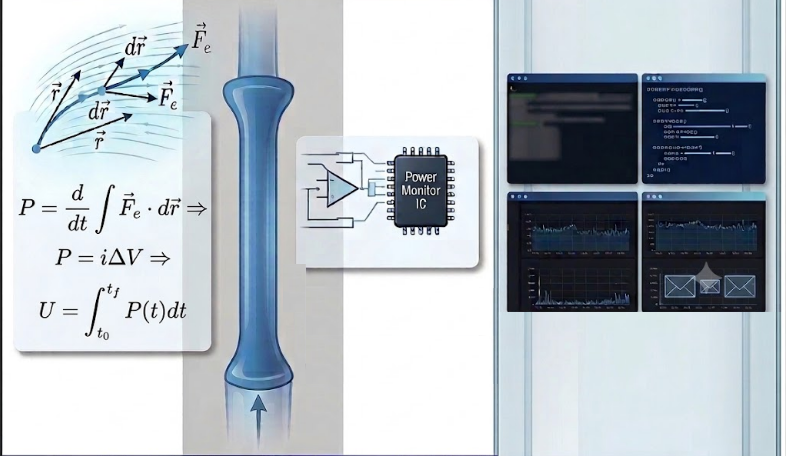
\includegraphics[width = \textwidth]{images/defensa/consumo.png}
        \caption{Niveles de abstracción en el análisis del consumo energético}
      \end{figure}
    \end{frame}

    \begin{frame}{Diseño físico de una base de datos}
      \begin{figure}
        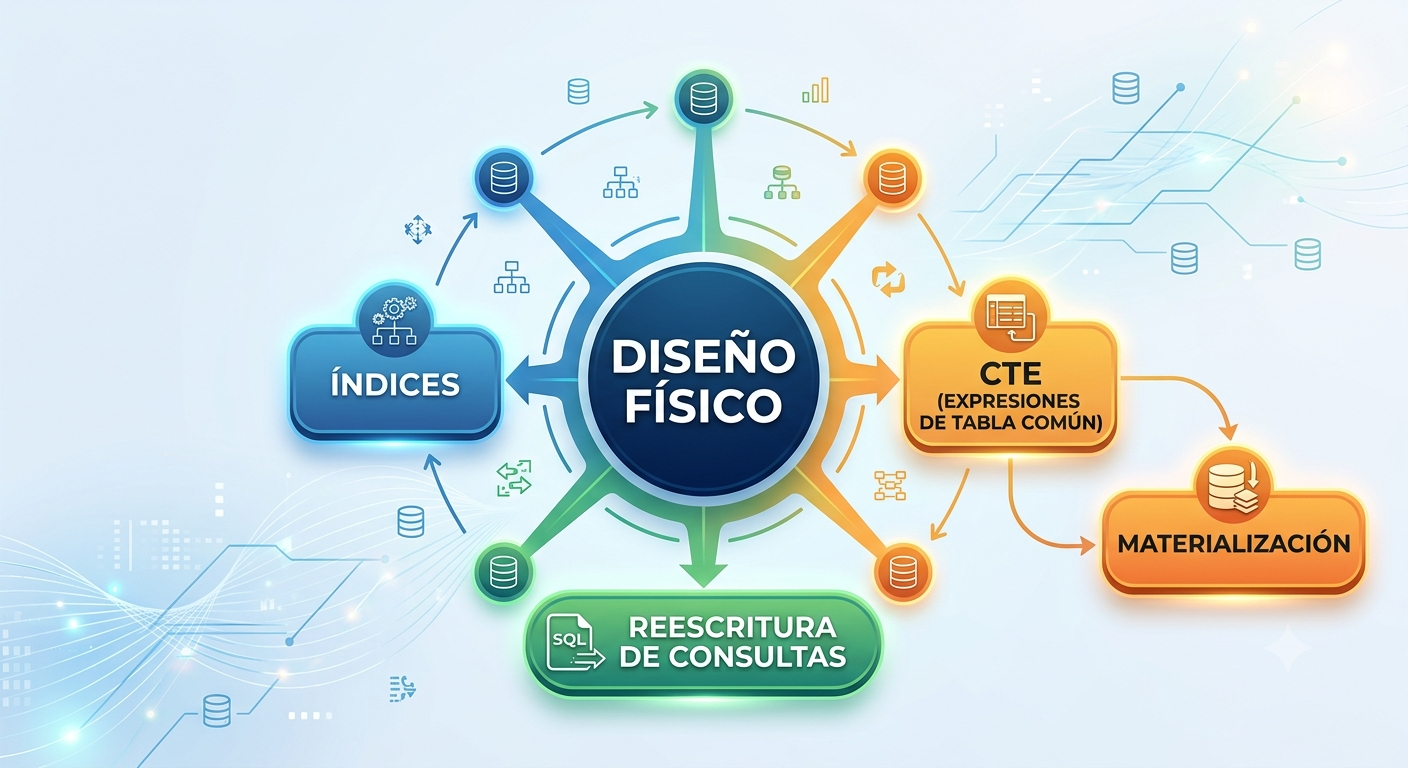
\includegraphics[width = \textwidth]{images/defensa/diseño.png}
        \caption{Herramientas de diseño}
      \end{figure}
    \end{frame}

    \begin{frame}{Gestión de memoria}
      \begin{figure}
        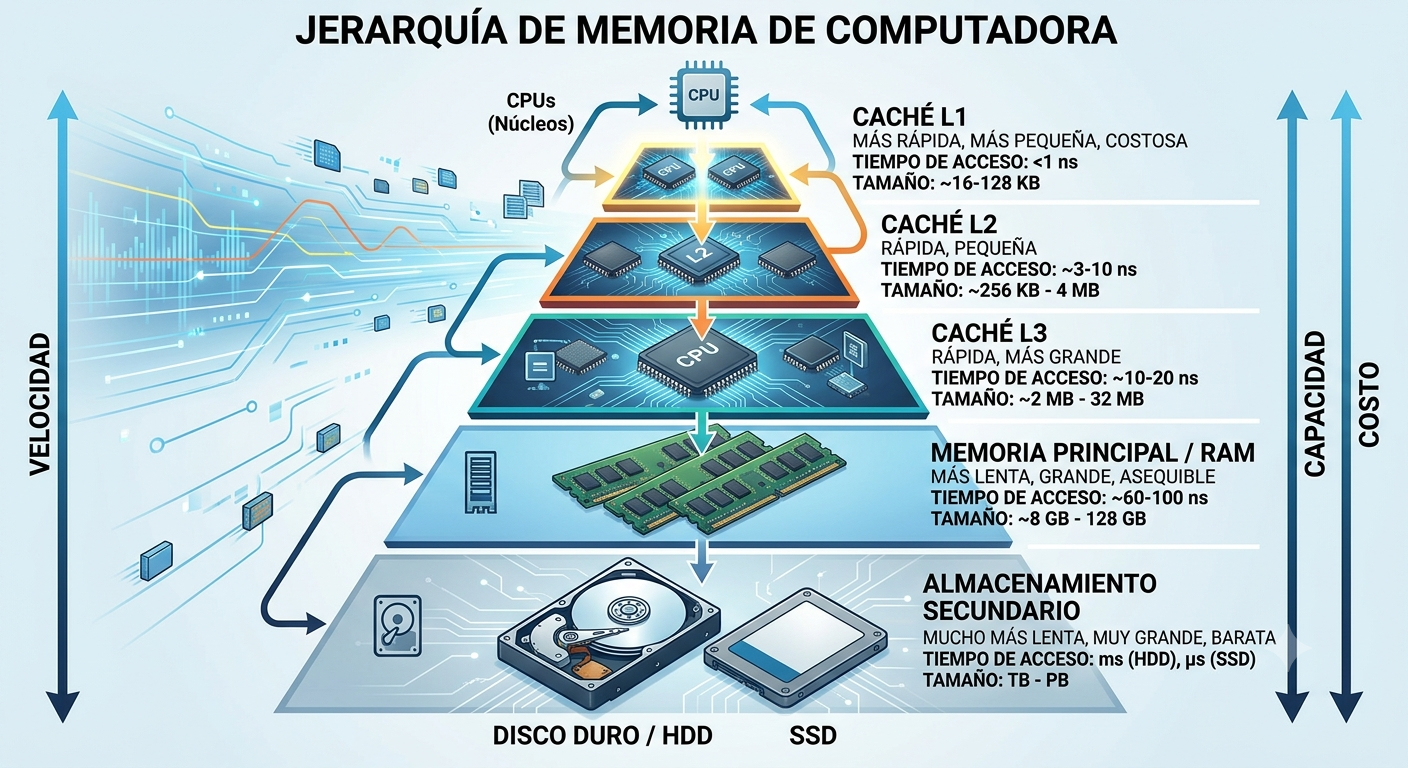
\includegraphics[width = \textwidth]{images/defensa/memoria.png}
        \caption{Jerarquía de memoria (pendiente)}
      \end{figure}
    \end{frame}

    \begin{frame}{\textit{Buffer Pool} y Problemas de Paginación}
      \begin{figure}
        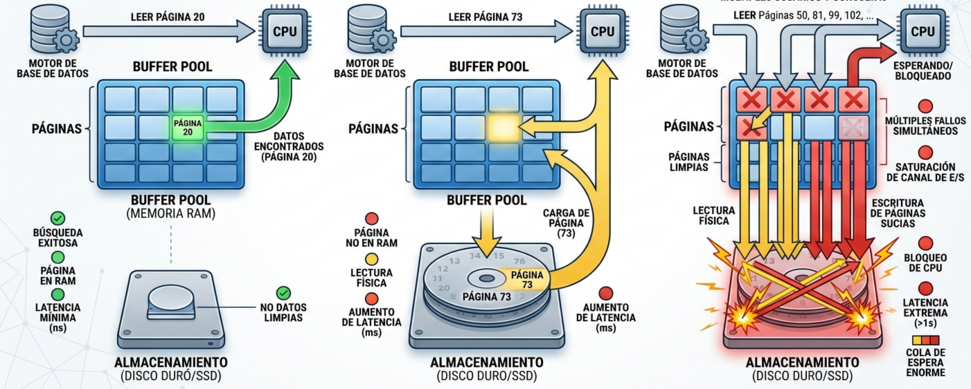
\includegraphics[width = \textwidth]{images/defensa/bufferpool.png}
        \caption{\textit{Buffer Pool}}
      \end{figure}
    \end{frame}

    \begin{frame}{Pruebas estadísticas}
      \renewcommand{\arraystretch}{4.0}
      $\begin{array}{l c c}
        Shapiro-Wilk & X \sim N(\mu, \sigma)                                  & W = \dfrac{\displaystyle \left ( \sum_{i = 1}^k a_i \left ( x_{(n-i+1)} - x_{(i)} \right ) \right ) ^ 2}{\displaystyle \sum_{i = 1}^n \left ( x_{(i)} - \bar{x} \right ) ^ 2} \nonumber \\
        Spearman     & X,Y \not\sim N(\mu, \sigma) \Rightarrow \rho(X, Y) = 0 & \rho = 1 - \dfrac{6 \sum d_i^2}{n(n^2-1)} \nonumber \\
        Kendall      & X,Y \not\sim N(\mu, \sigma) \Rightarrow \tau(X, Y) = 0 & \tau = 2 \dfrac{C - D}{n(n - 1)} \nonumber
      \end{array}$
    \end{frame}

  % section marcos_teórico_y_tecnológico (end)

  \section{Marco Tecnológico y Metodología Experimental} % (fold)
  \label{sec:marco_tecnológico_y_metodología_experimental}
    \begin{frame}{Base de datos}
      \begin{figure}
        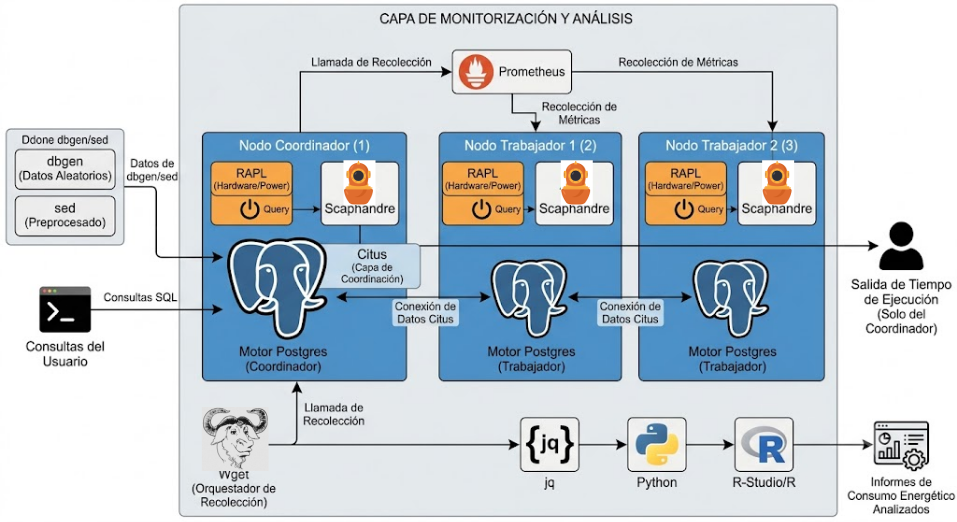
\includegraphics[width = \textwidth]{images/defensa/arquitectura.png}
        \caption{\textit{Arquitectura}}
      \end{figure}
    \end{frame}

    \begin{frame}{Experimentos y Estrategia de diseño}
      \begin{table}
        \tiny
        \caption{Consultas de la base de datos TPC-H}
        \begin{tabular}{c c c}
          \textbf{Consulta} & \textbf{Característica}                                                         & \textbf{Estrategia}                    \\ \hline
          1                 & Alta agregación y filtros                                                       & Reescritura con CTE y literal de fecha \\ \hline
          2                 & Multi-\texttt{JOIN} distribuido con subconsulta correlacionada                  & Índices                                \\ \hline
          3                 & Multi-\texttt{JOIN} con ordenamiento post agregación                            & Índices                                \\ \hline
          4                 & \texttt{SEMI-JOIN} masivo                                                       & Índices                                \\ \hline
          5                 & Multi-\texttt{JOIN} con ordenamiento post agregación                            & Índices                                \\ \hline
          6                 & Lectura secuencial con filtrado de rangos selectivo (sin agrupación)            & Índices                                \\ \hline
          7                 & Multi-\texttt{JOIN} con cálculos y extracción de fechas                         & Índices                                \\ \hline
          8                 & Multi-\texttt{JOIN} con agregación condicional segmentada                       & Índices                                \\ \hline
          9                 & \texttt{JOIN} masivo con (\texttt{LIKE})                                        & Índices                                \\ \hline
          10                & Multi-\texttt{JOIN} con agrupación de alta cardinalidad                         & Índices                                \\ \hline
          11                & \texttt{JOIN} con subconsulta de agregación en la cláusula \texttt{HAVING}      & Índices                                \\ \hline
          12                & \texttt{JOIN} simple con evaluación condicional masiva (\texttt{CASE WHEN})     & Índices                                \\ \hline
          13                & \texttt{LEFT OUTER JOIN} con agregaciones anidadas                              & Reescritura con CTE                    \\ \hline
          14                & \texttt{JOIN} simple con agregación condicional basada en  (\texttt{LIKE})      & Índices                                \\ \hline
          15                & Creación de vista temporal seguida de agregación por valor máximo               & Índices                                \\ \hline
          16                & \texttt{ANTI-JOIN} con conteo de valores distintos (\texttt{COUNT DISTINCT})    & Reescritura con CTE                    \\ \hline
          17                & \texttt{JOIN} simple ahogado por una subconsulta correlacionada de promedios    & Índices                                \\ \hline
          18                & Filtrado de alta cardinalidad en \texttt{IN} basado en una subconsulta agregada & Co-locación e índices                  \\ \hline
          19                & \texttt{JOIN} simple dominado por bloque de lógica condicional                  & Co-locación e índices                  \\ \hline
          20                & \texttt{JOIN} dependiente de subconsultas profundamente anidadas                & Índices                                \\ \hline
          21                & Multi-\texttt{JOIN} acoplado a \texttt{SEMI-JOIN} y \texttt{ANTI-JOIN}          & Índices                                \\ \hline
          22                & Agregación filtrada por \texttt{ANTI-JOIN} y extracción de subcadenas           & Índices                                \\ \hline
        \end{tabular}
      \end{table}
    \end{frame}
  % section metodología_experimental (end)

  \section{Resultados} % (fold)
  \label{sec:resultados}
    \subsection{Tamaño de la base de datos} % (fold)
    \label{sub:tamaño_de_la_base_de_datos}
      \begin{frame}{Con diseño vs Sin diseño}
        \begin{figure}
          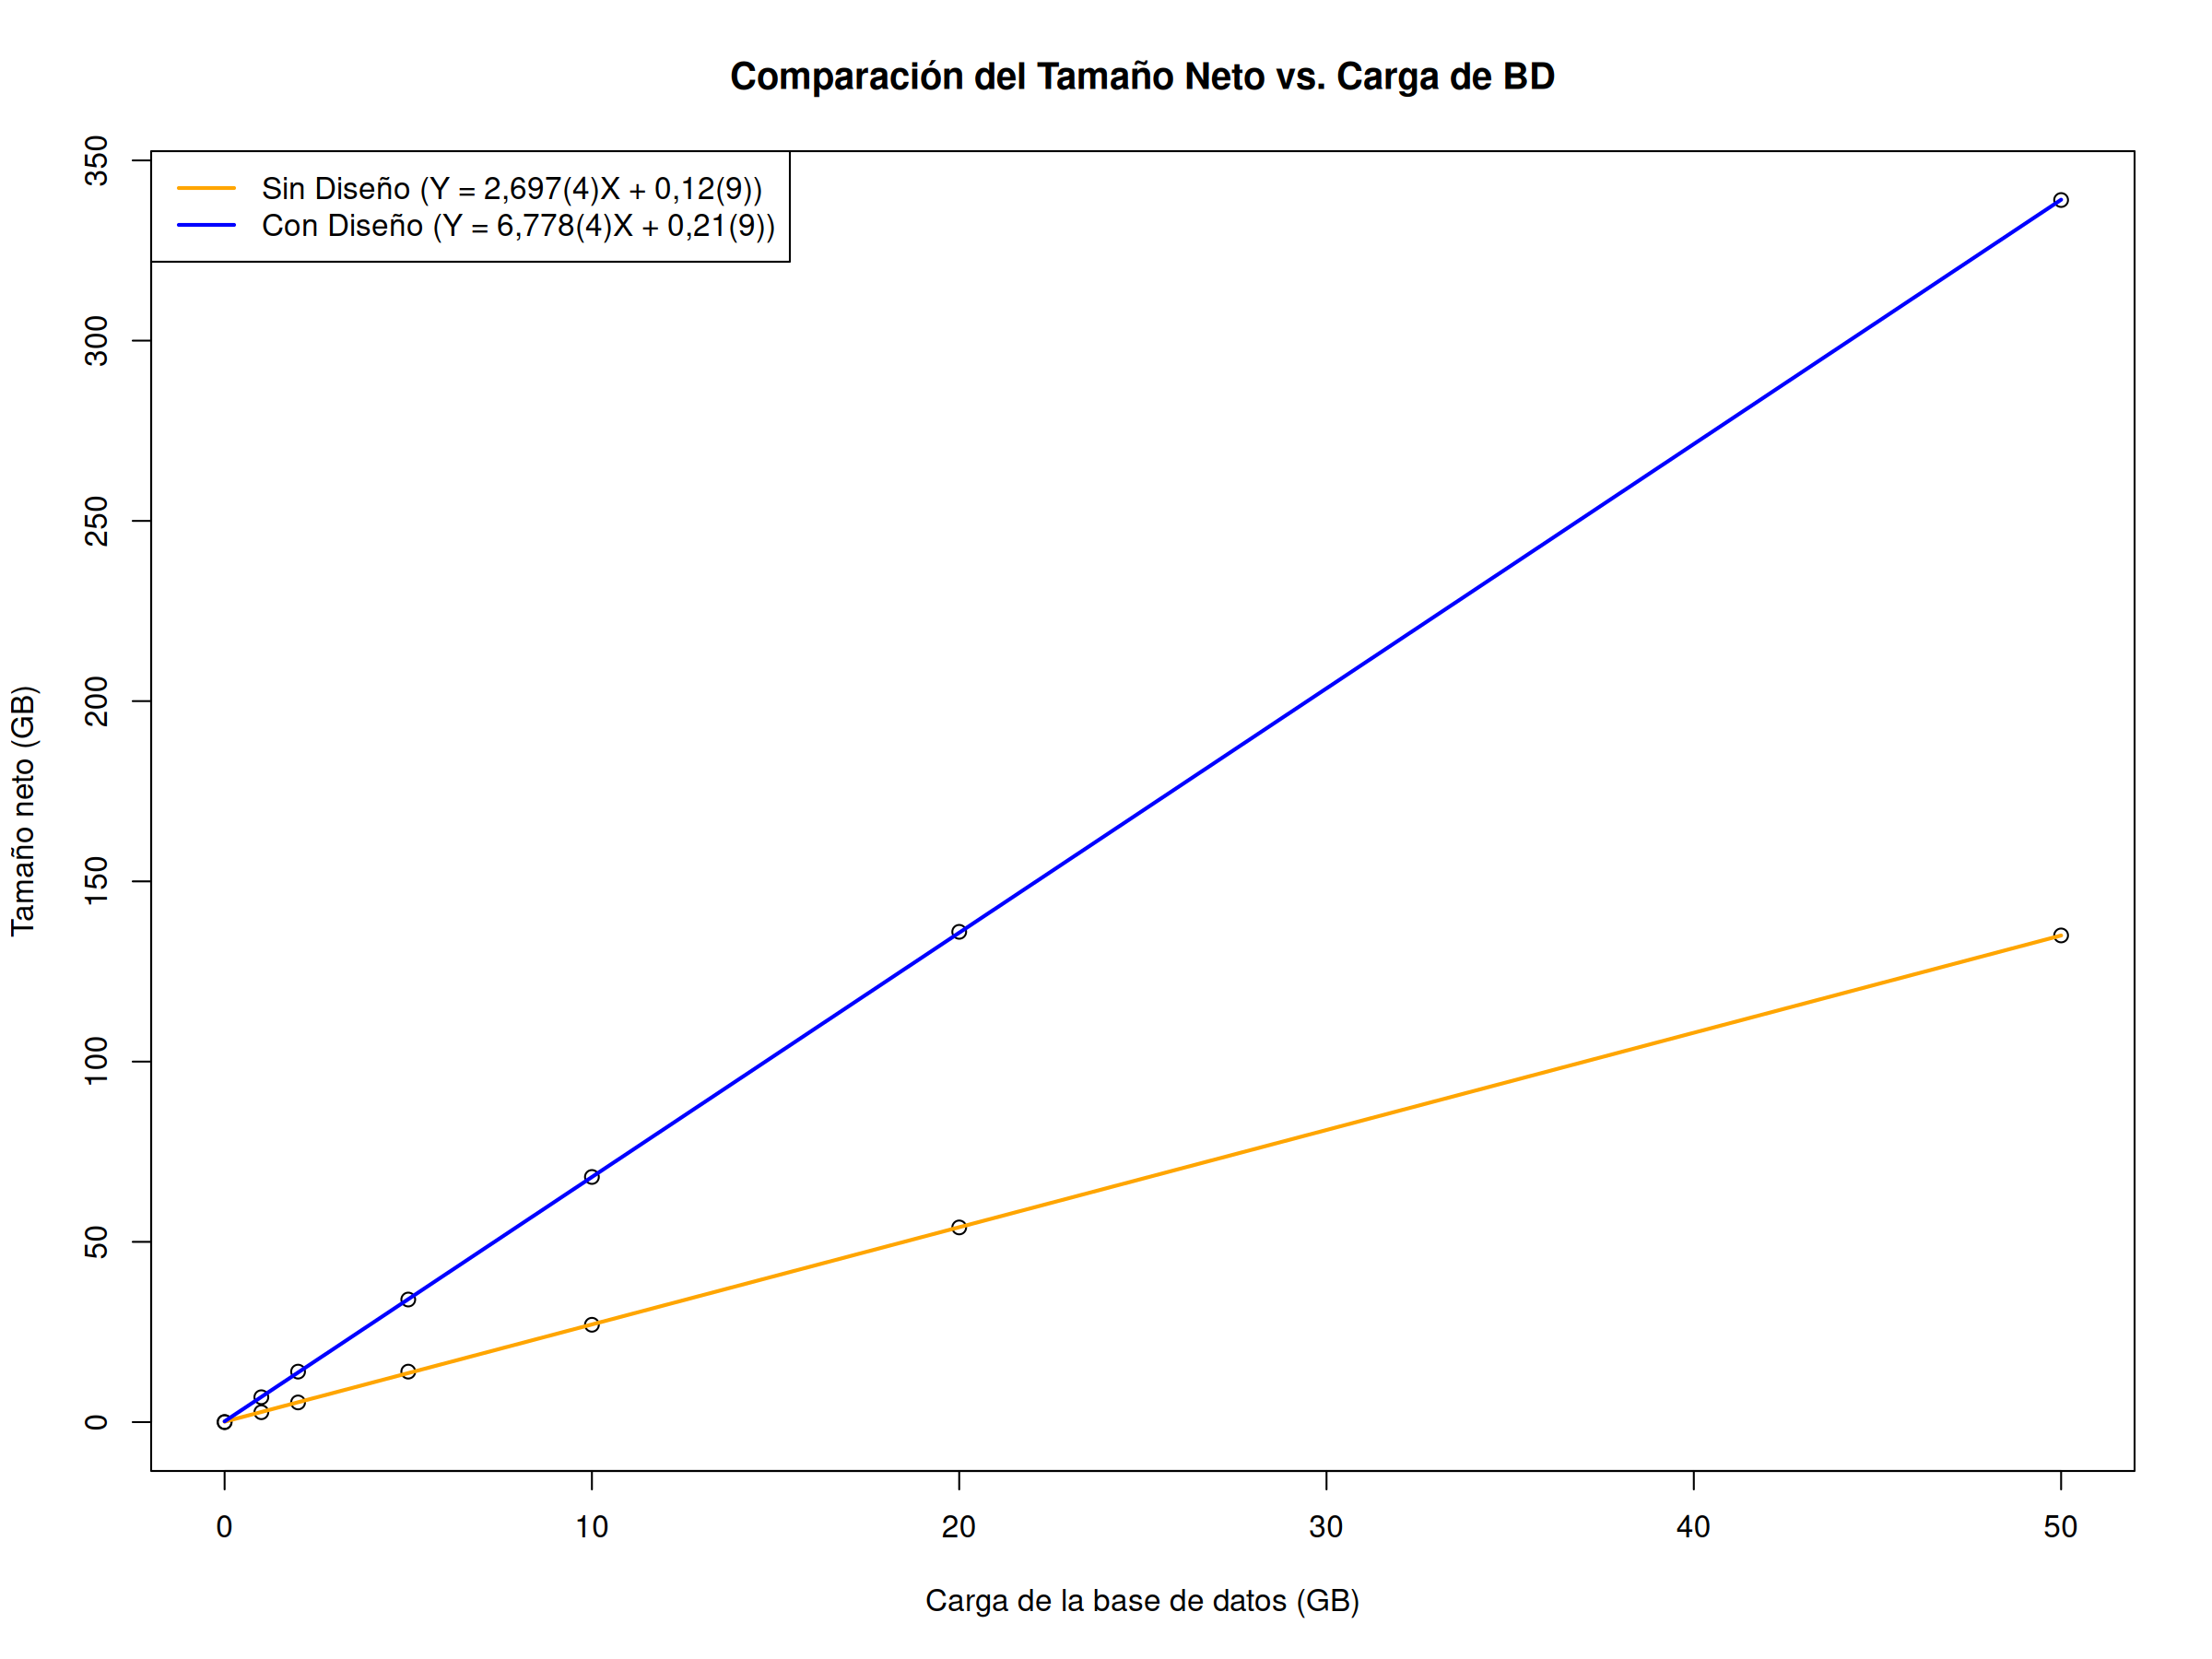
\includegraphics[width = 0.49\textwidth]{images/defensa/tamaño.png}
          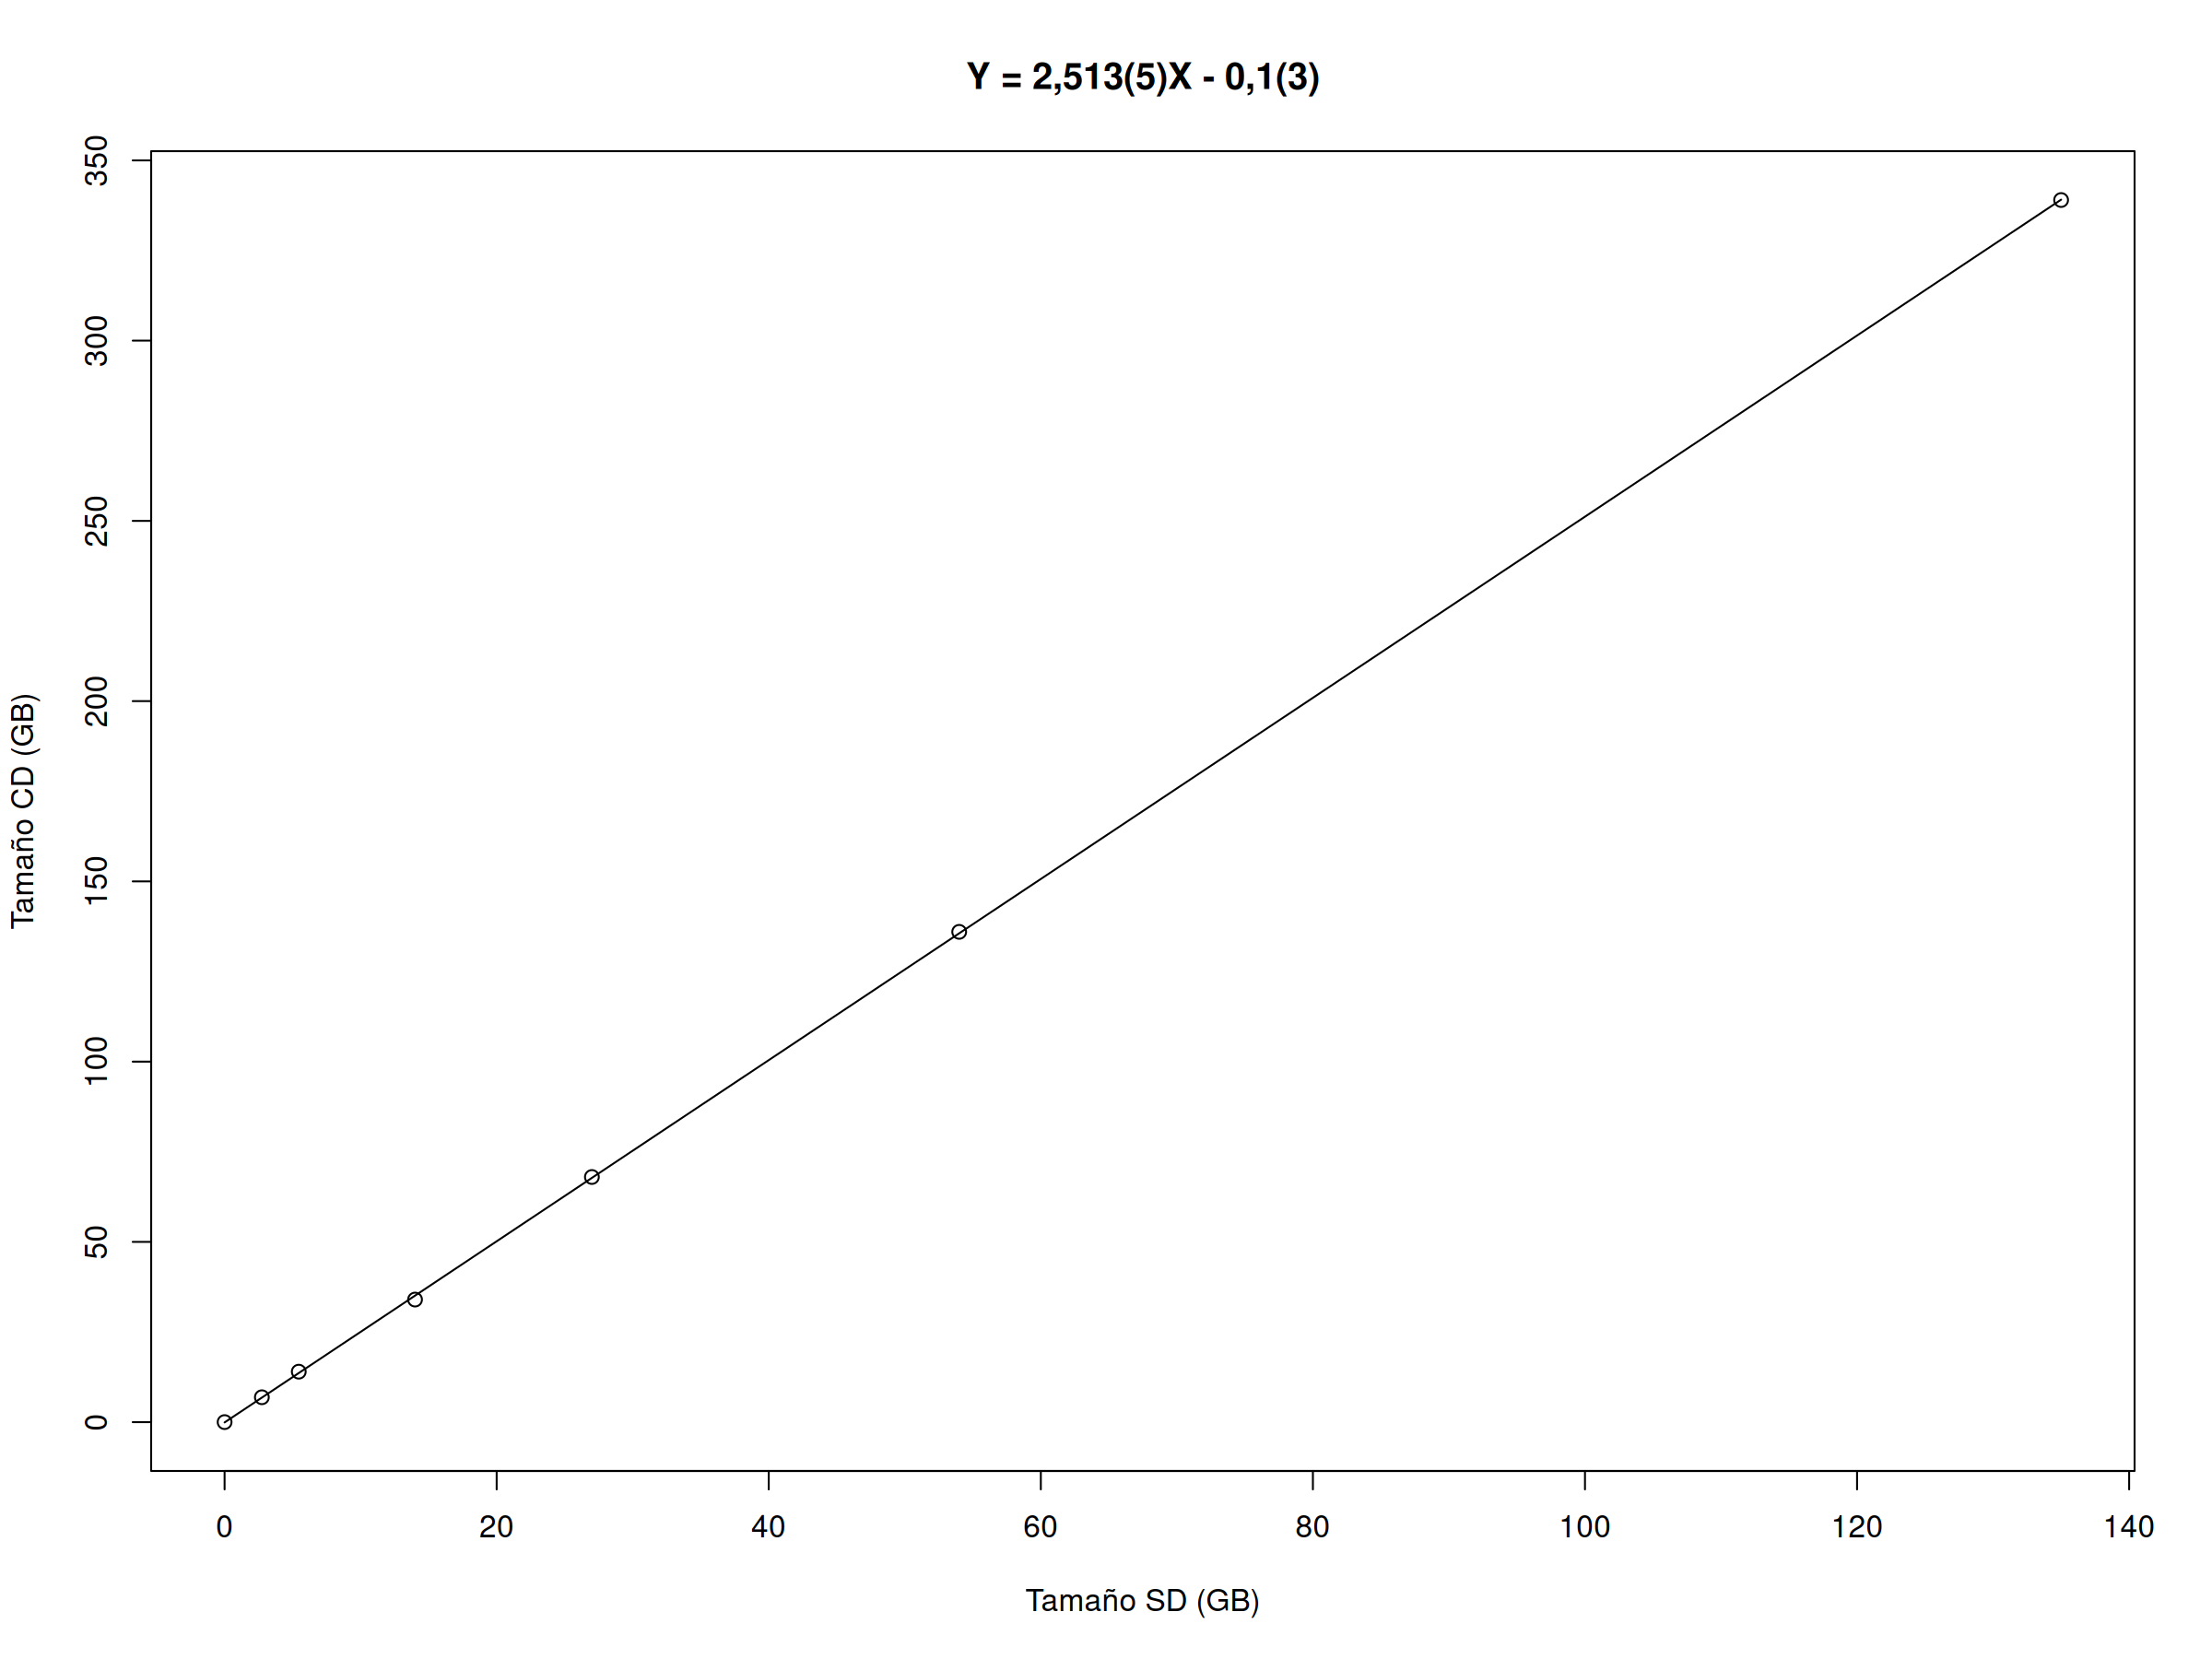
\includegraphics[width = 0.49\textwidth]{images/defensa/CDvsSD.png}
          \caption{Regresiones lineales de los tamaños de las bases de datos}
        \end{figure}
      \end{frame}
    % subsection tamaño_de_la_base_de_datos (end)

    \subsection{Rendimiento} % (fold)
    \label{sub:rendimiento}
      \begin{frame}{Consultas rápidas}
        \begin{figure}
          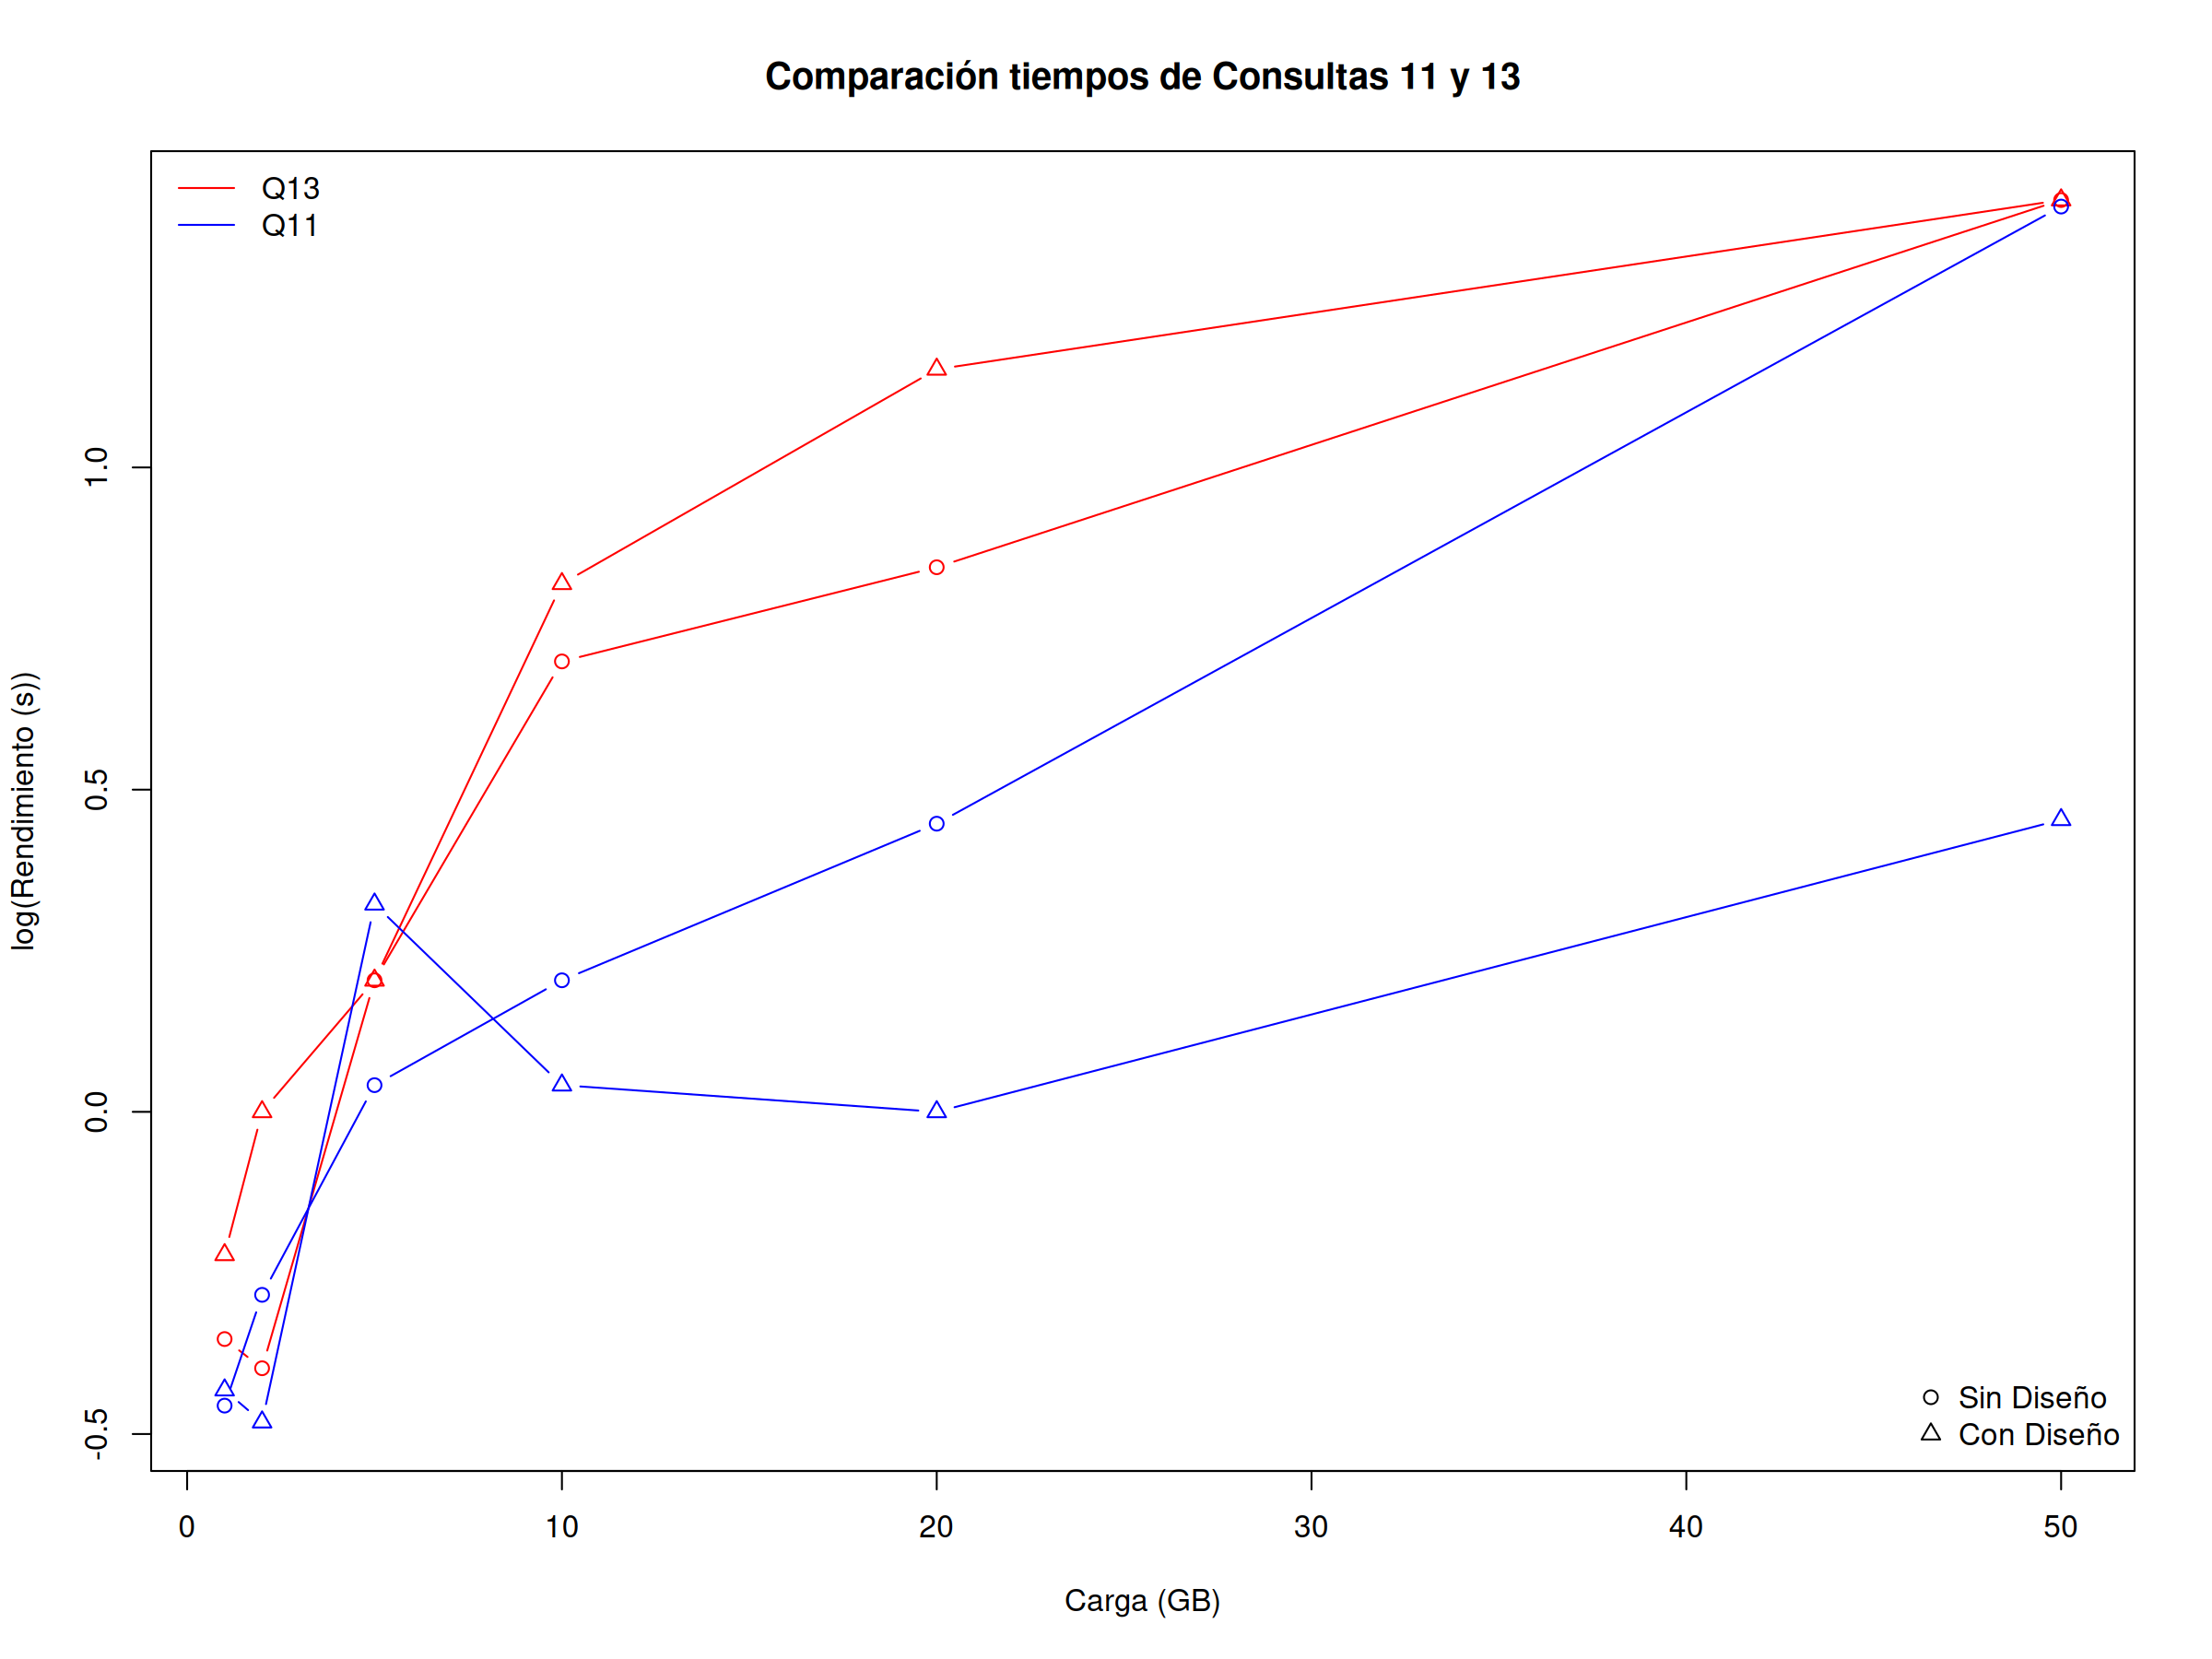
\includegraphics[width = 0.49\textwidth]{images/defensa/tRapidas1.png}
          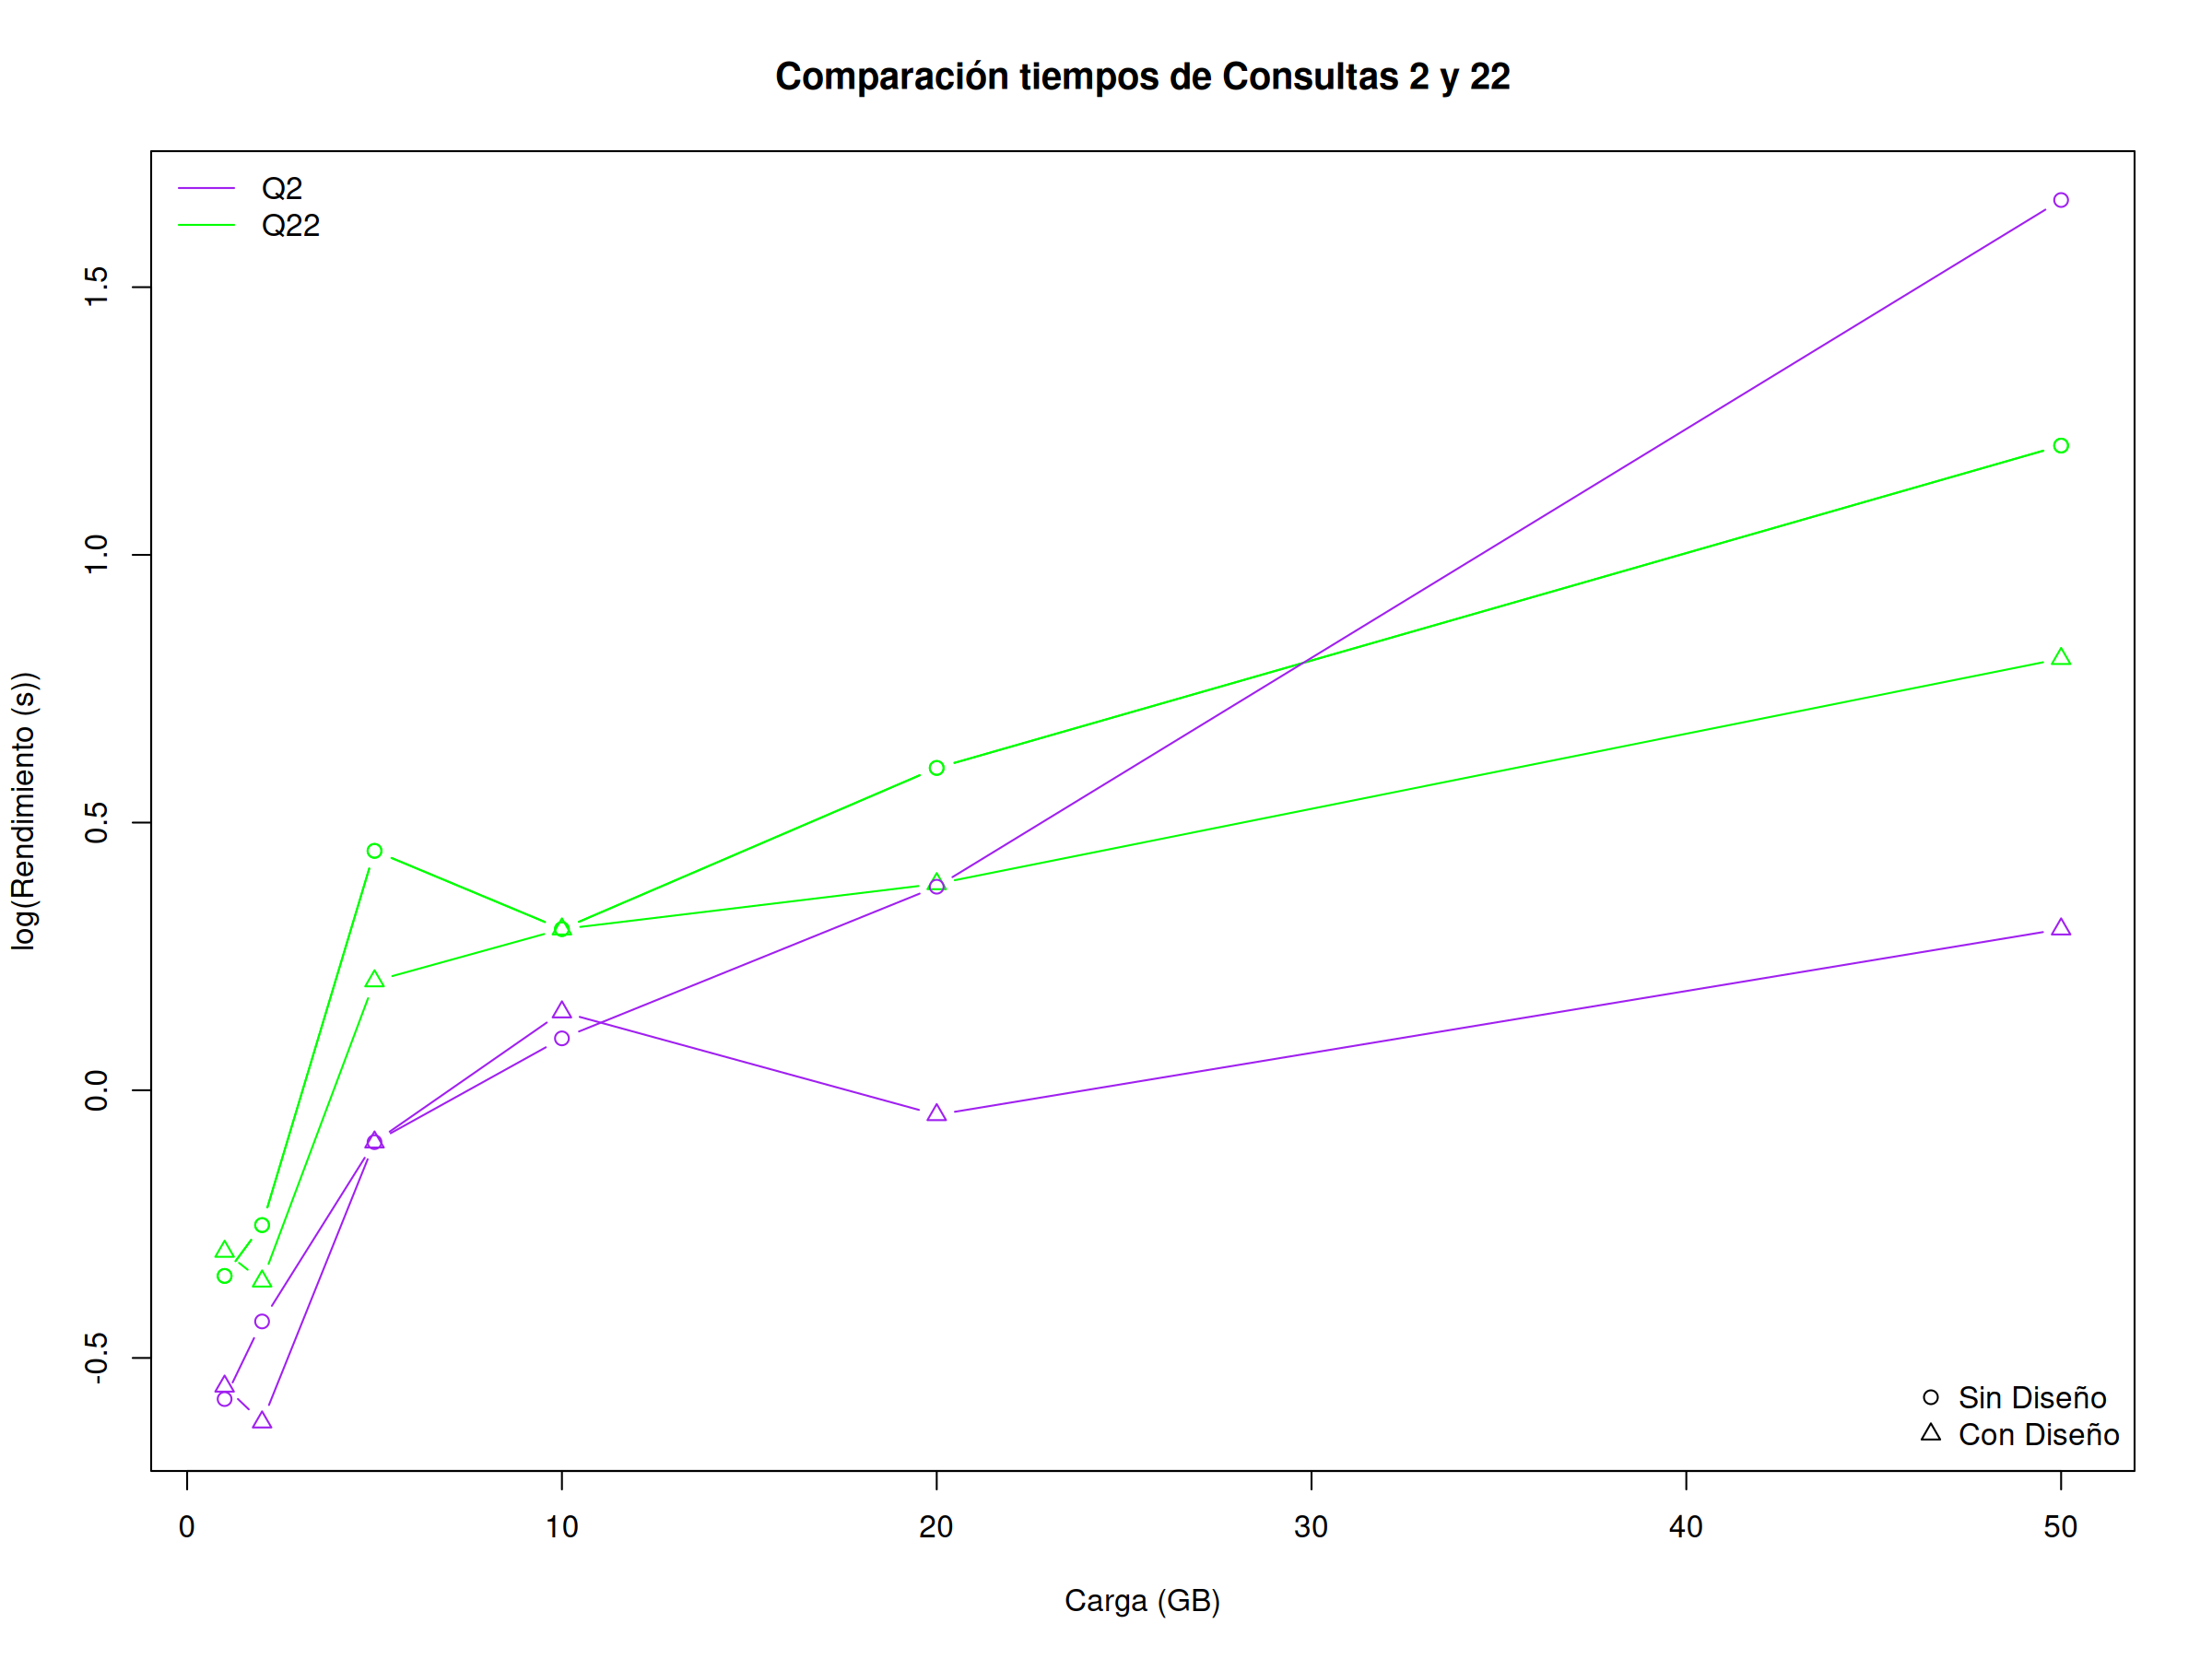
\includegraphics[width = 0.49\textwidth]{images/defensa/tRapidas2.png}
          \caption{Comparación de tiempos consultas rápidas}
        \end{figure}
      \end{frame}

      \begin{frame}{Consultas intermedias}
        \begin{figure}
          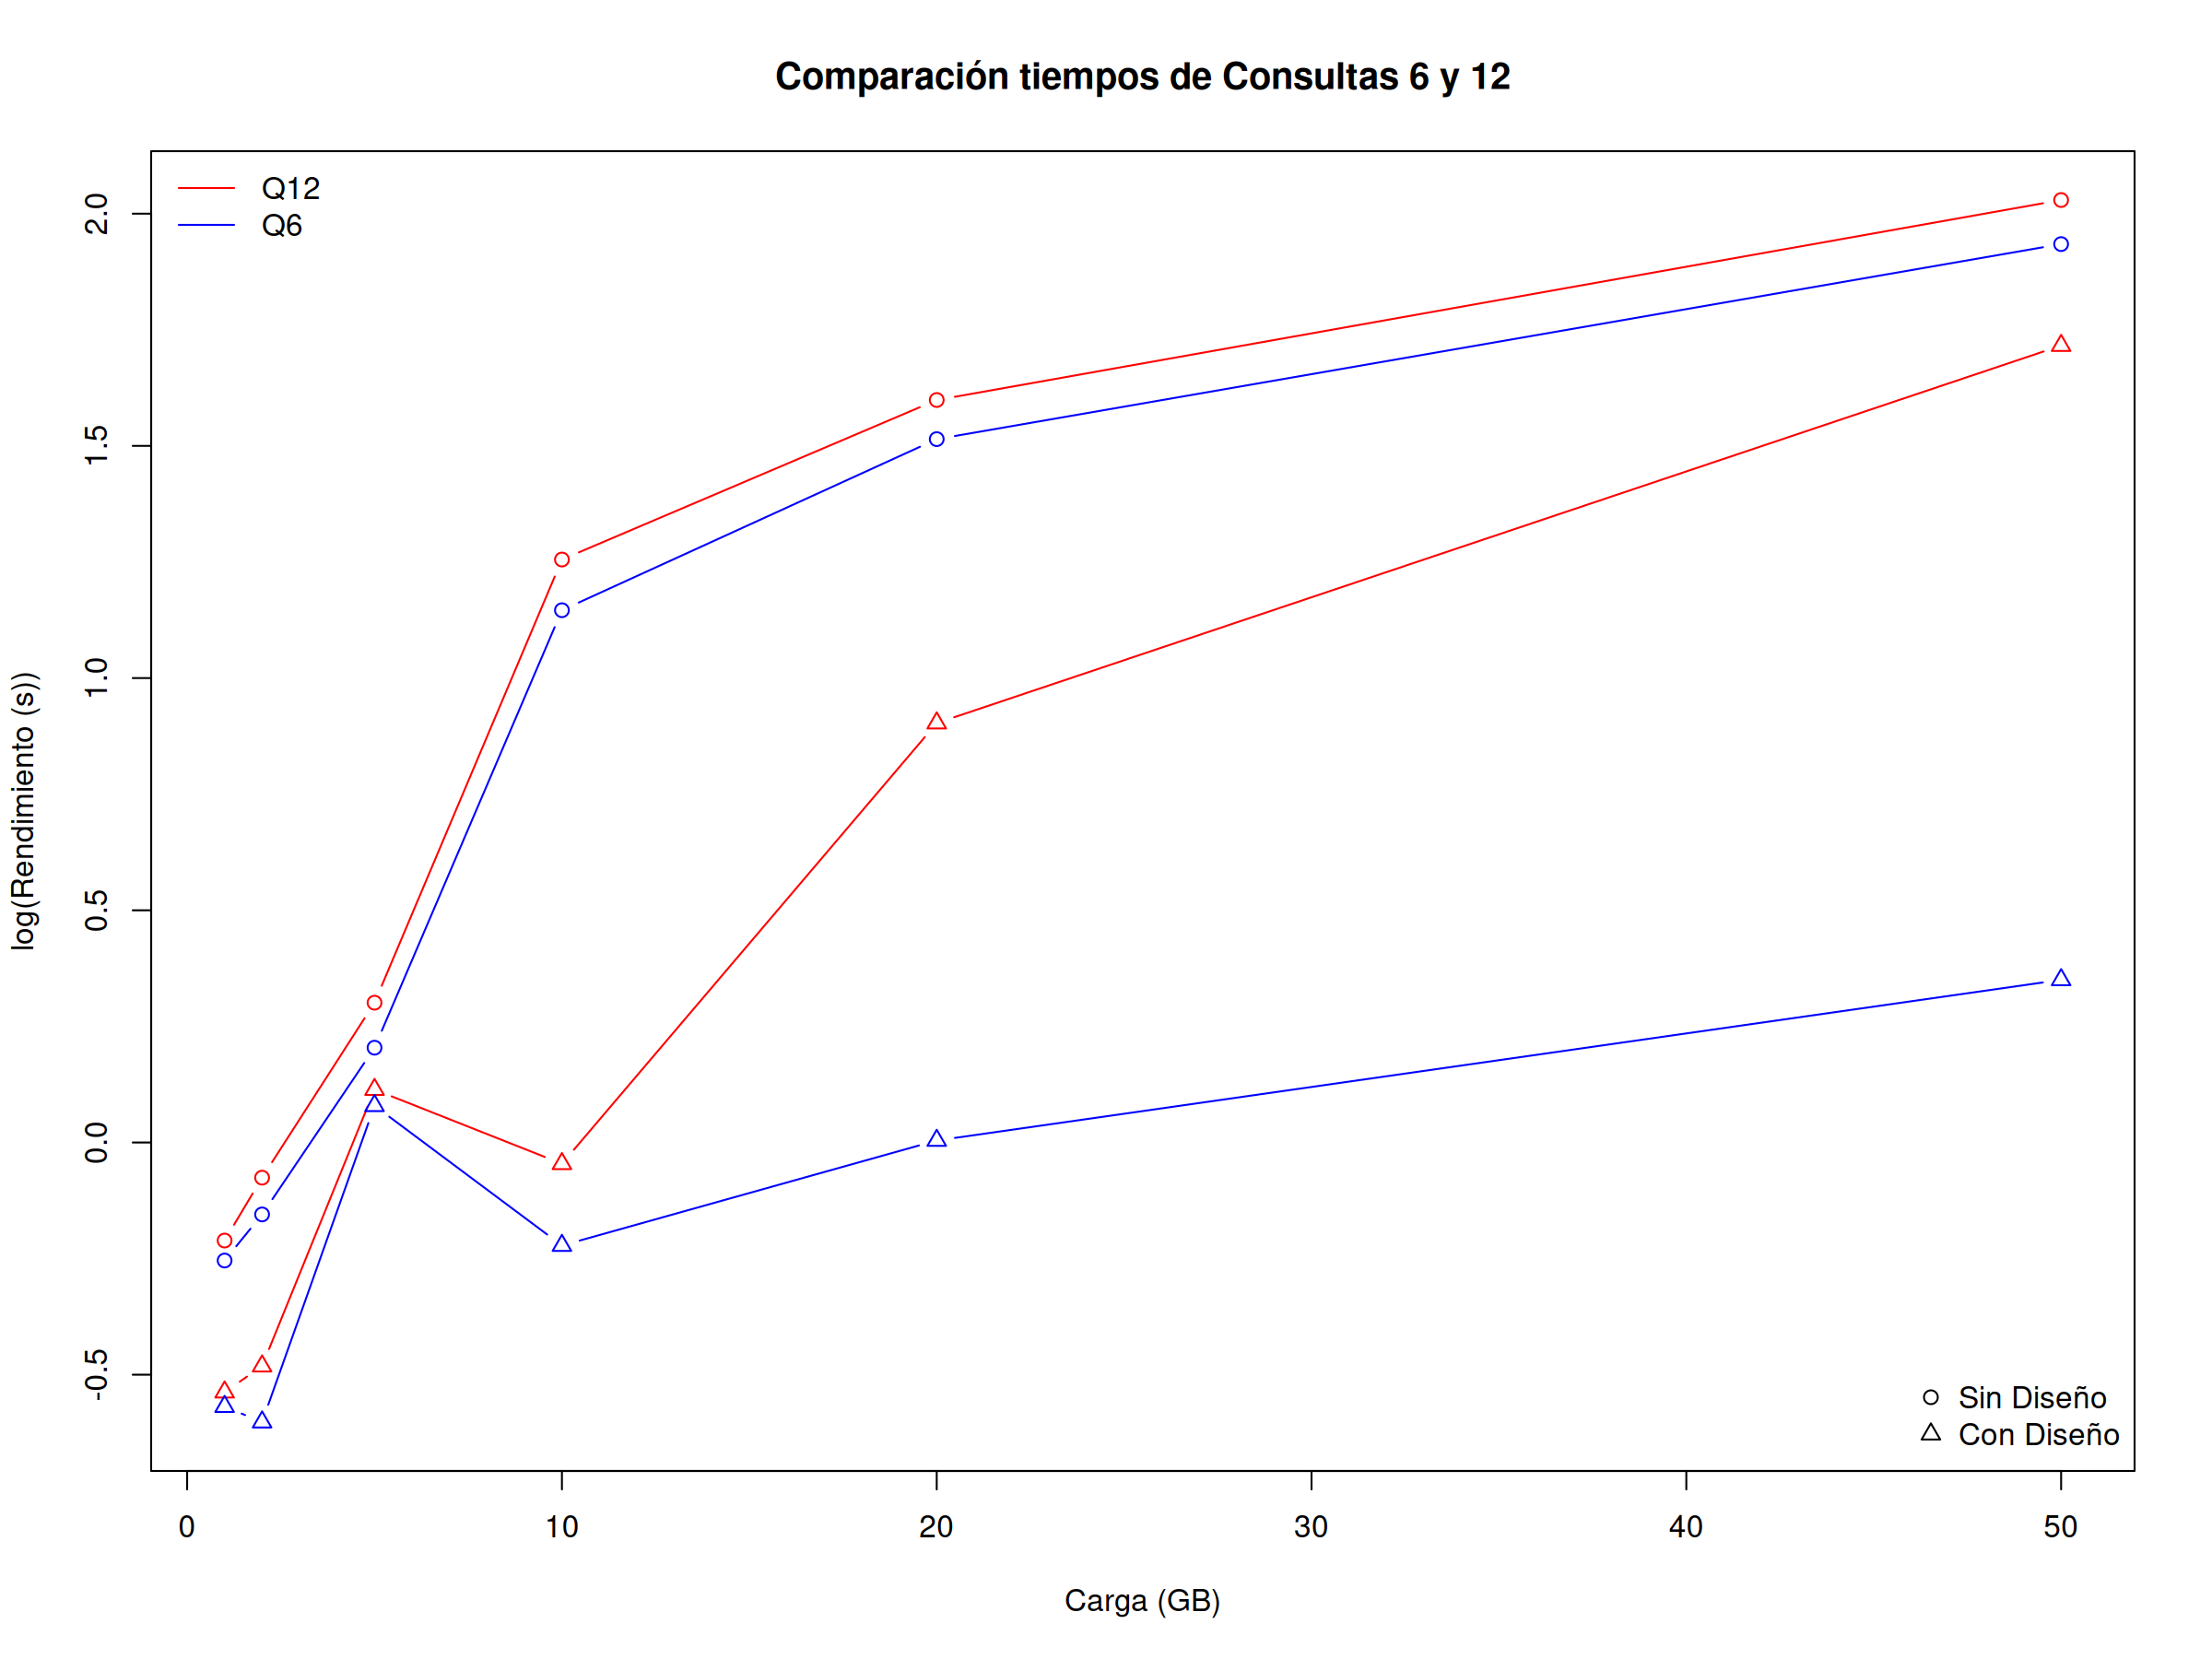
\includegraphics[width = 0.49\textwidth]{images/defensa/tMediaBaja1}
          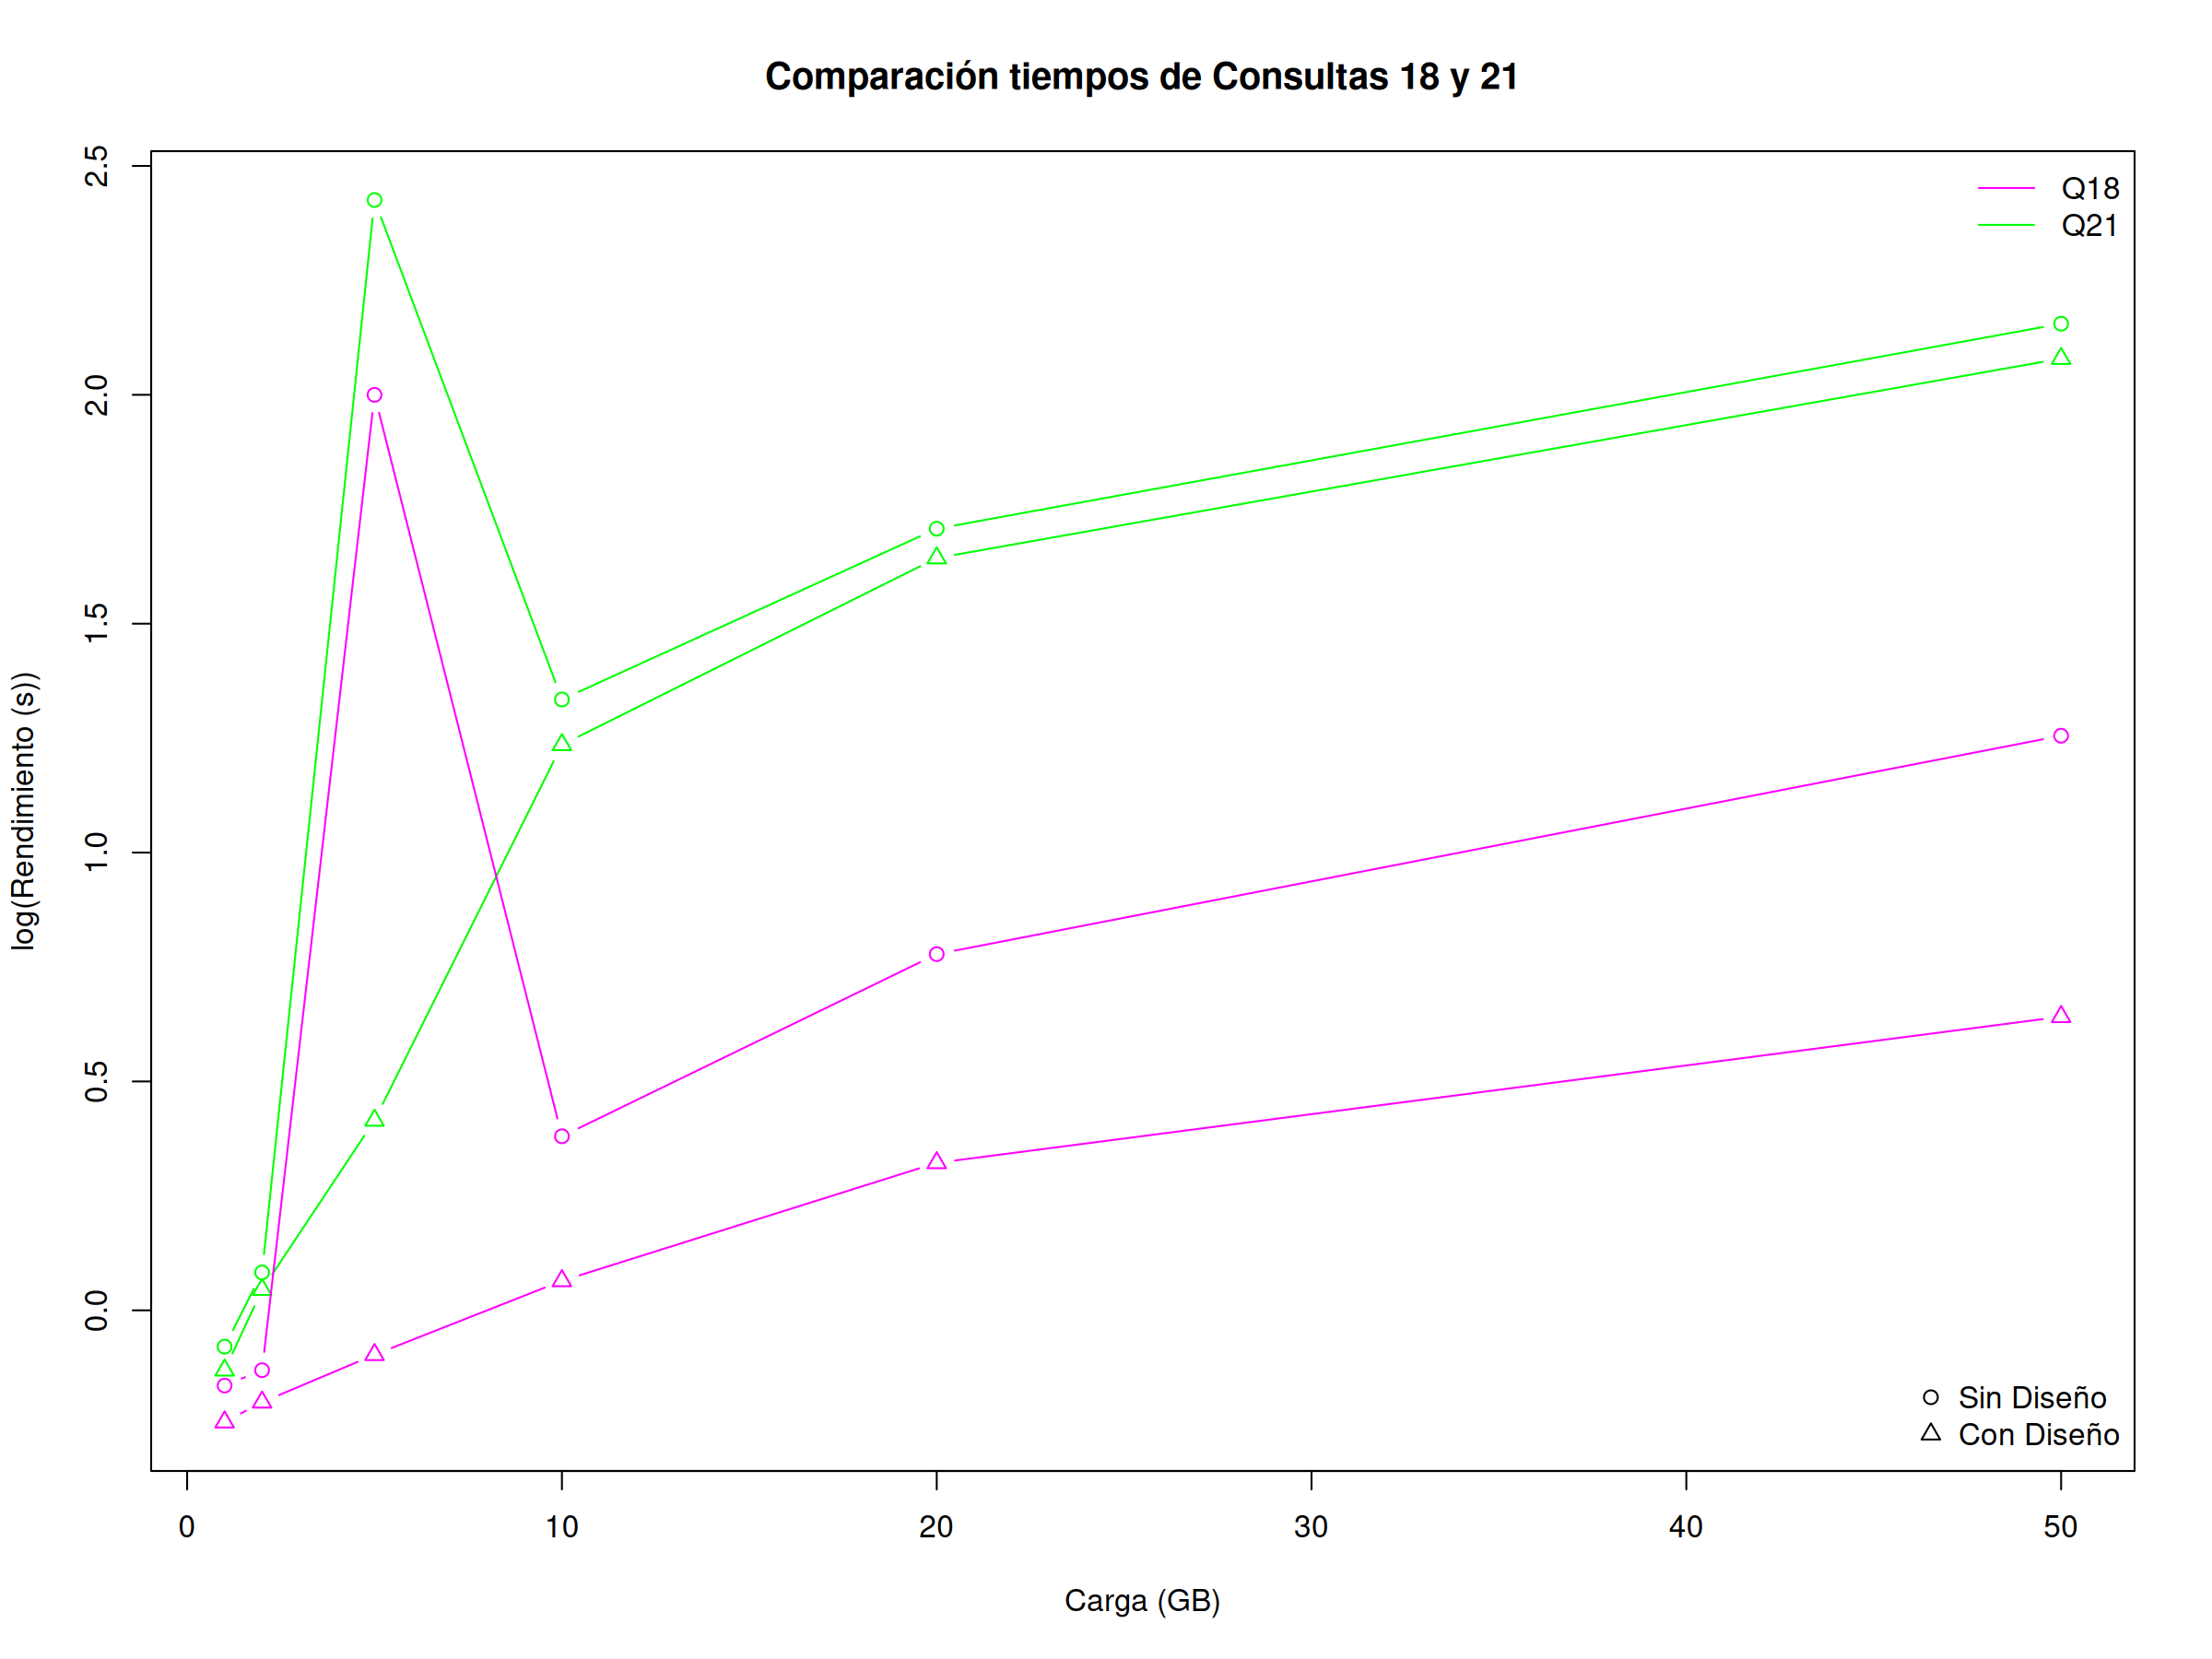
\includegraphics[width = 0.49\textwidth]{images/defensa/tMediaBaja2}
          \caption{Comparación de tiempos consultas intermedias}
        \end{figure}
      \end{frame}

      \begin{frame}{Consultas intermedias}
        \begin{figure}
          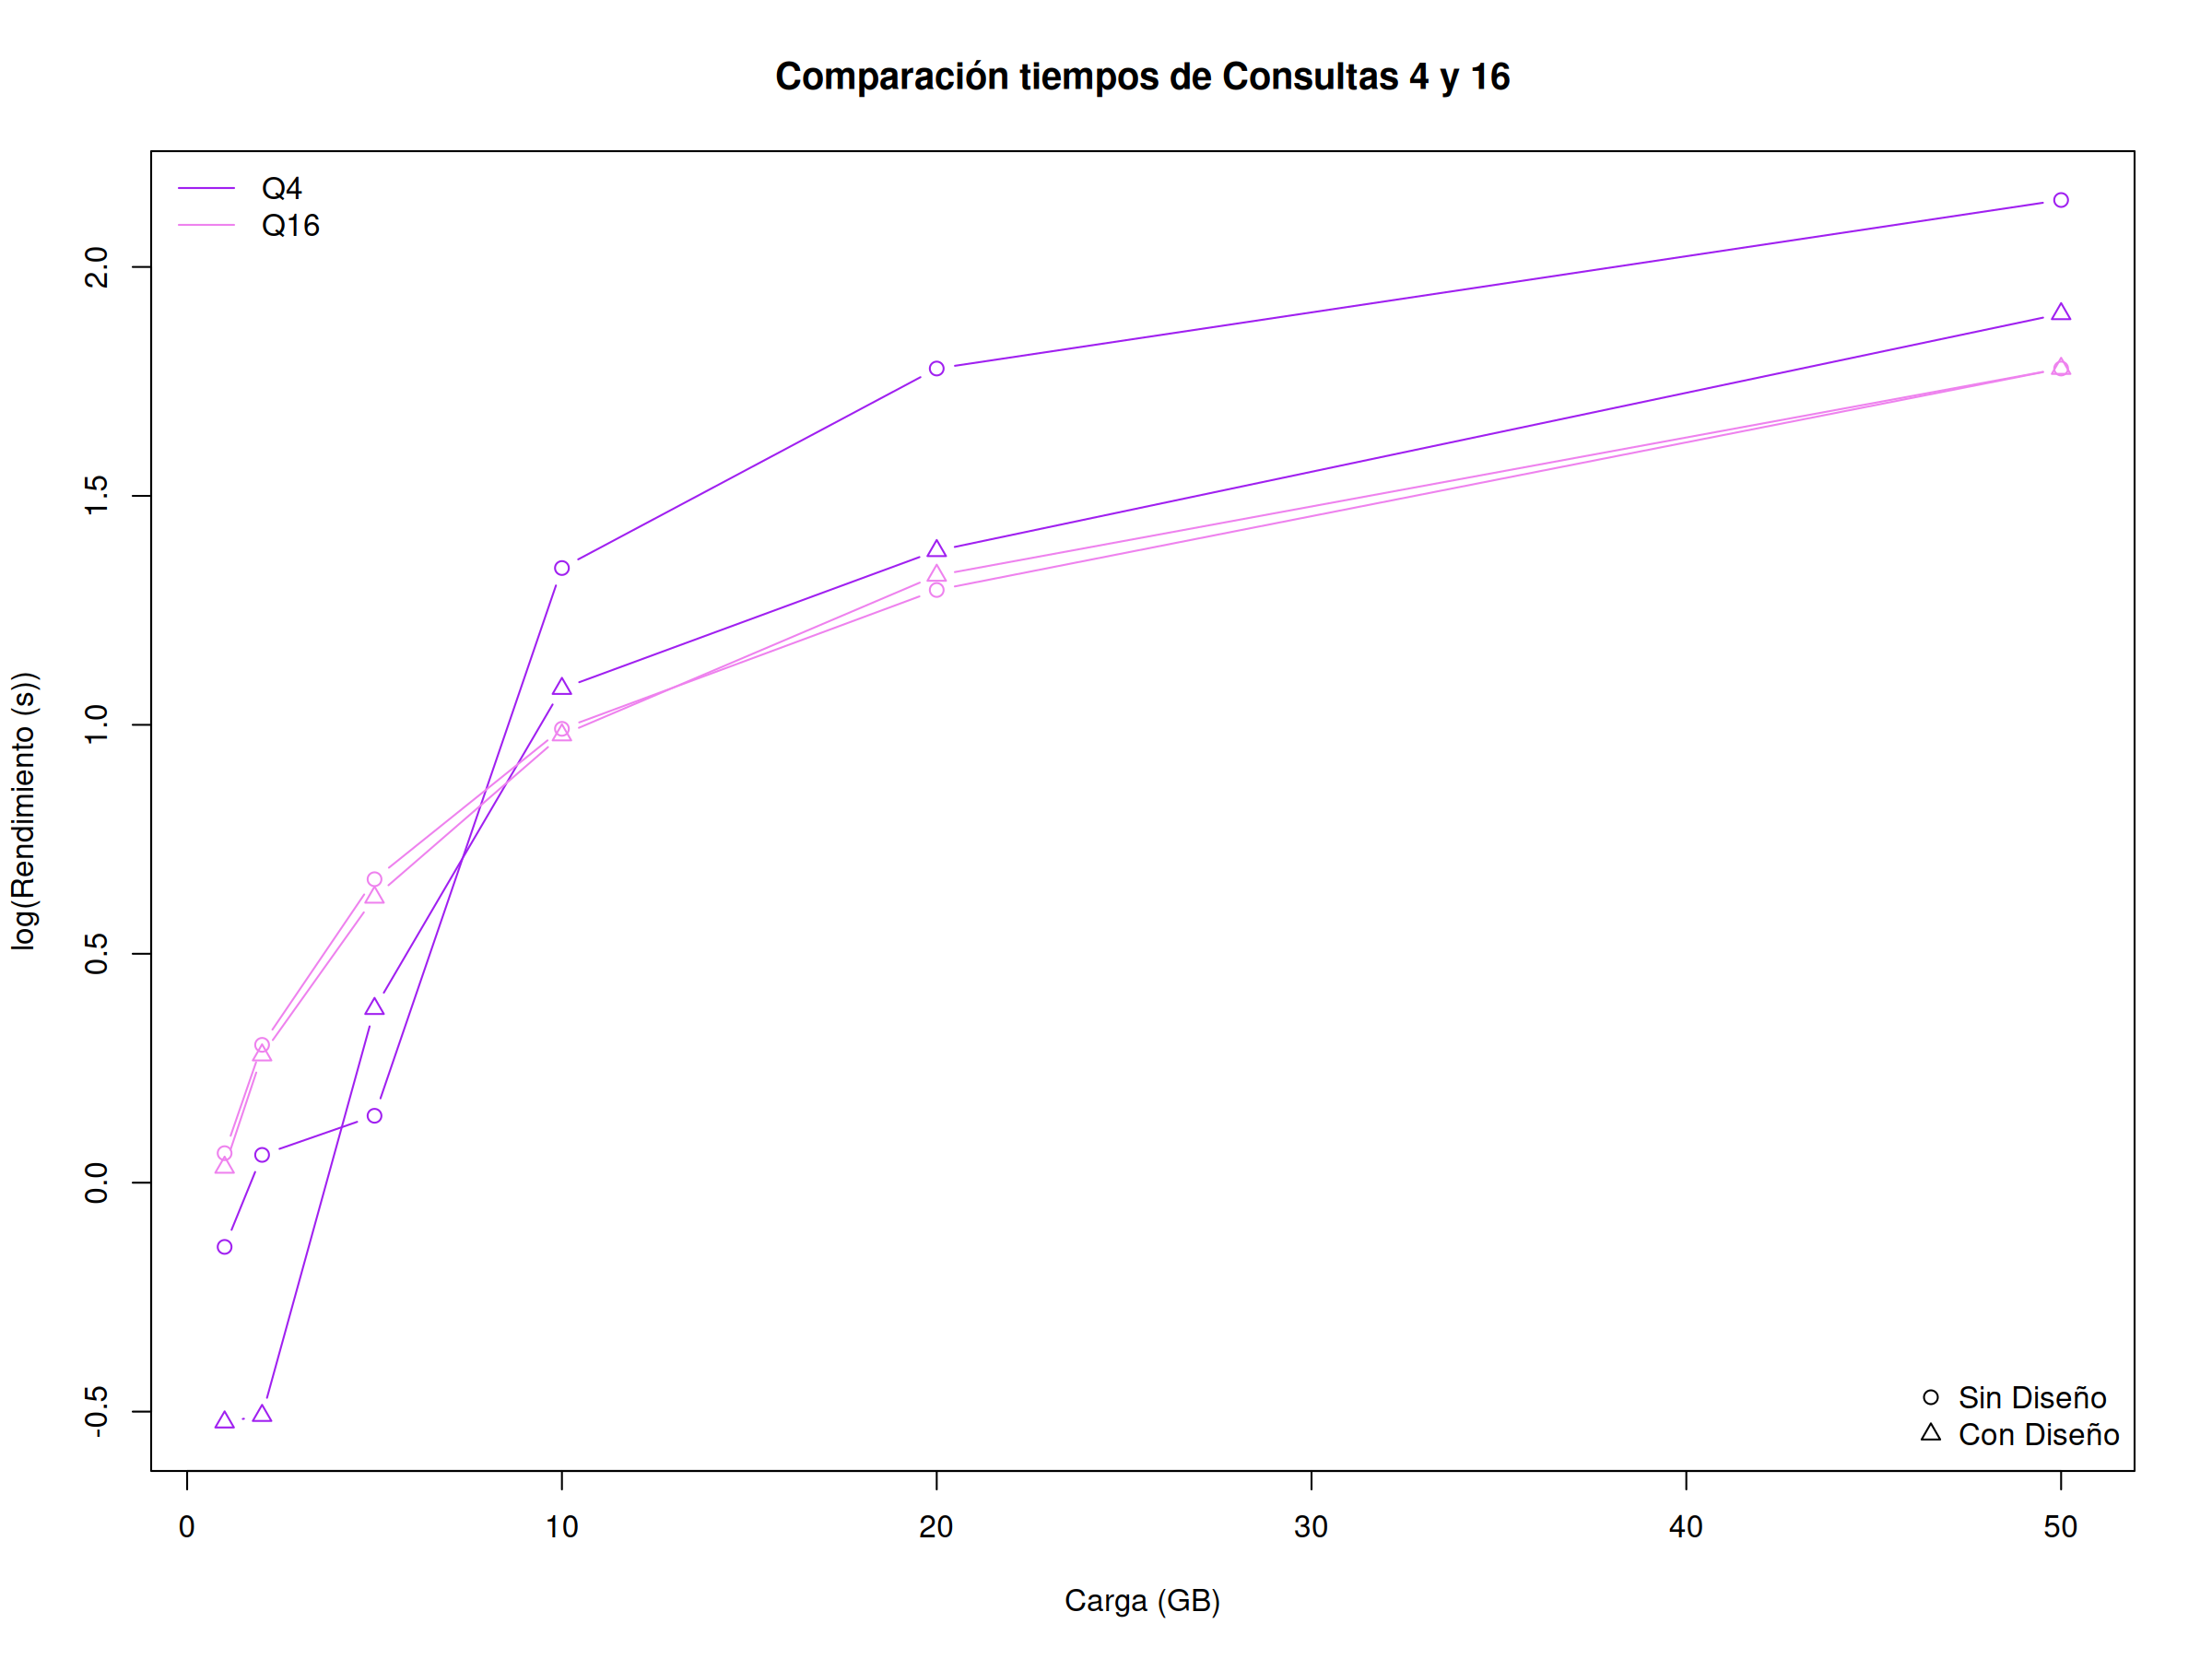
\includegraphics[width = 0.49\textwidth]{images/defensa/tMediaBaja3}
          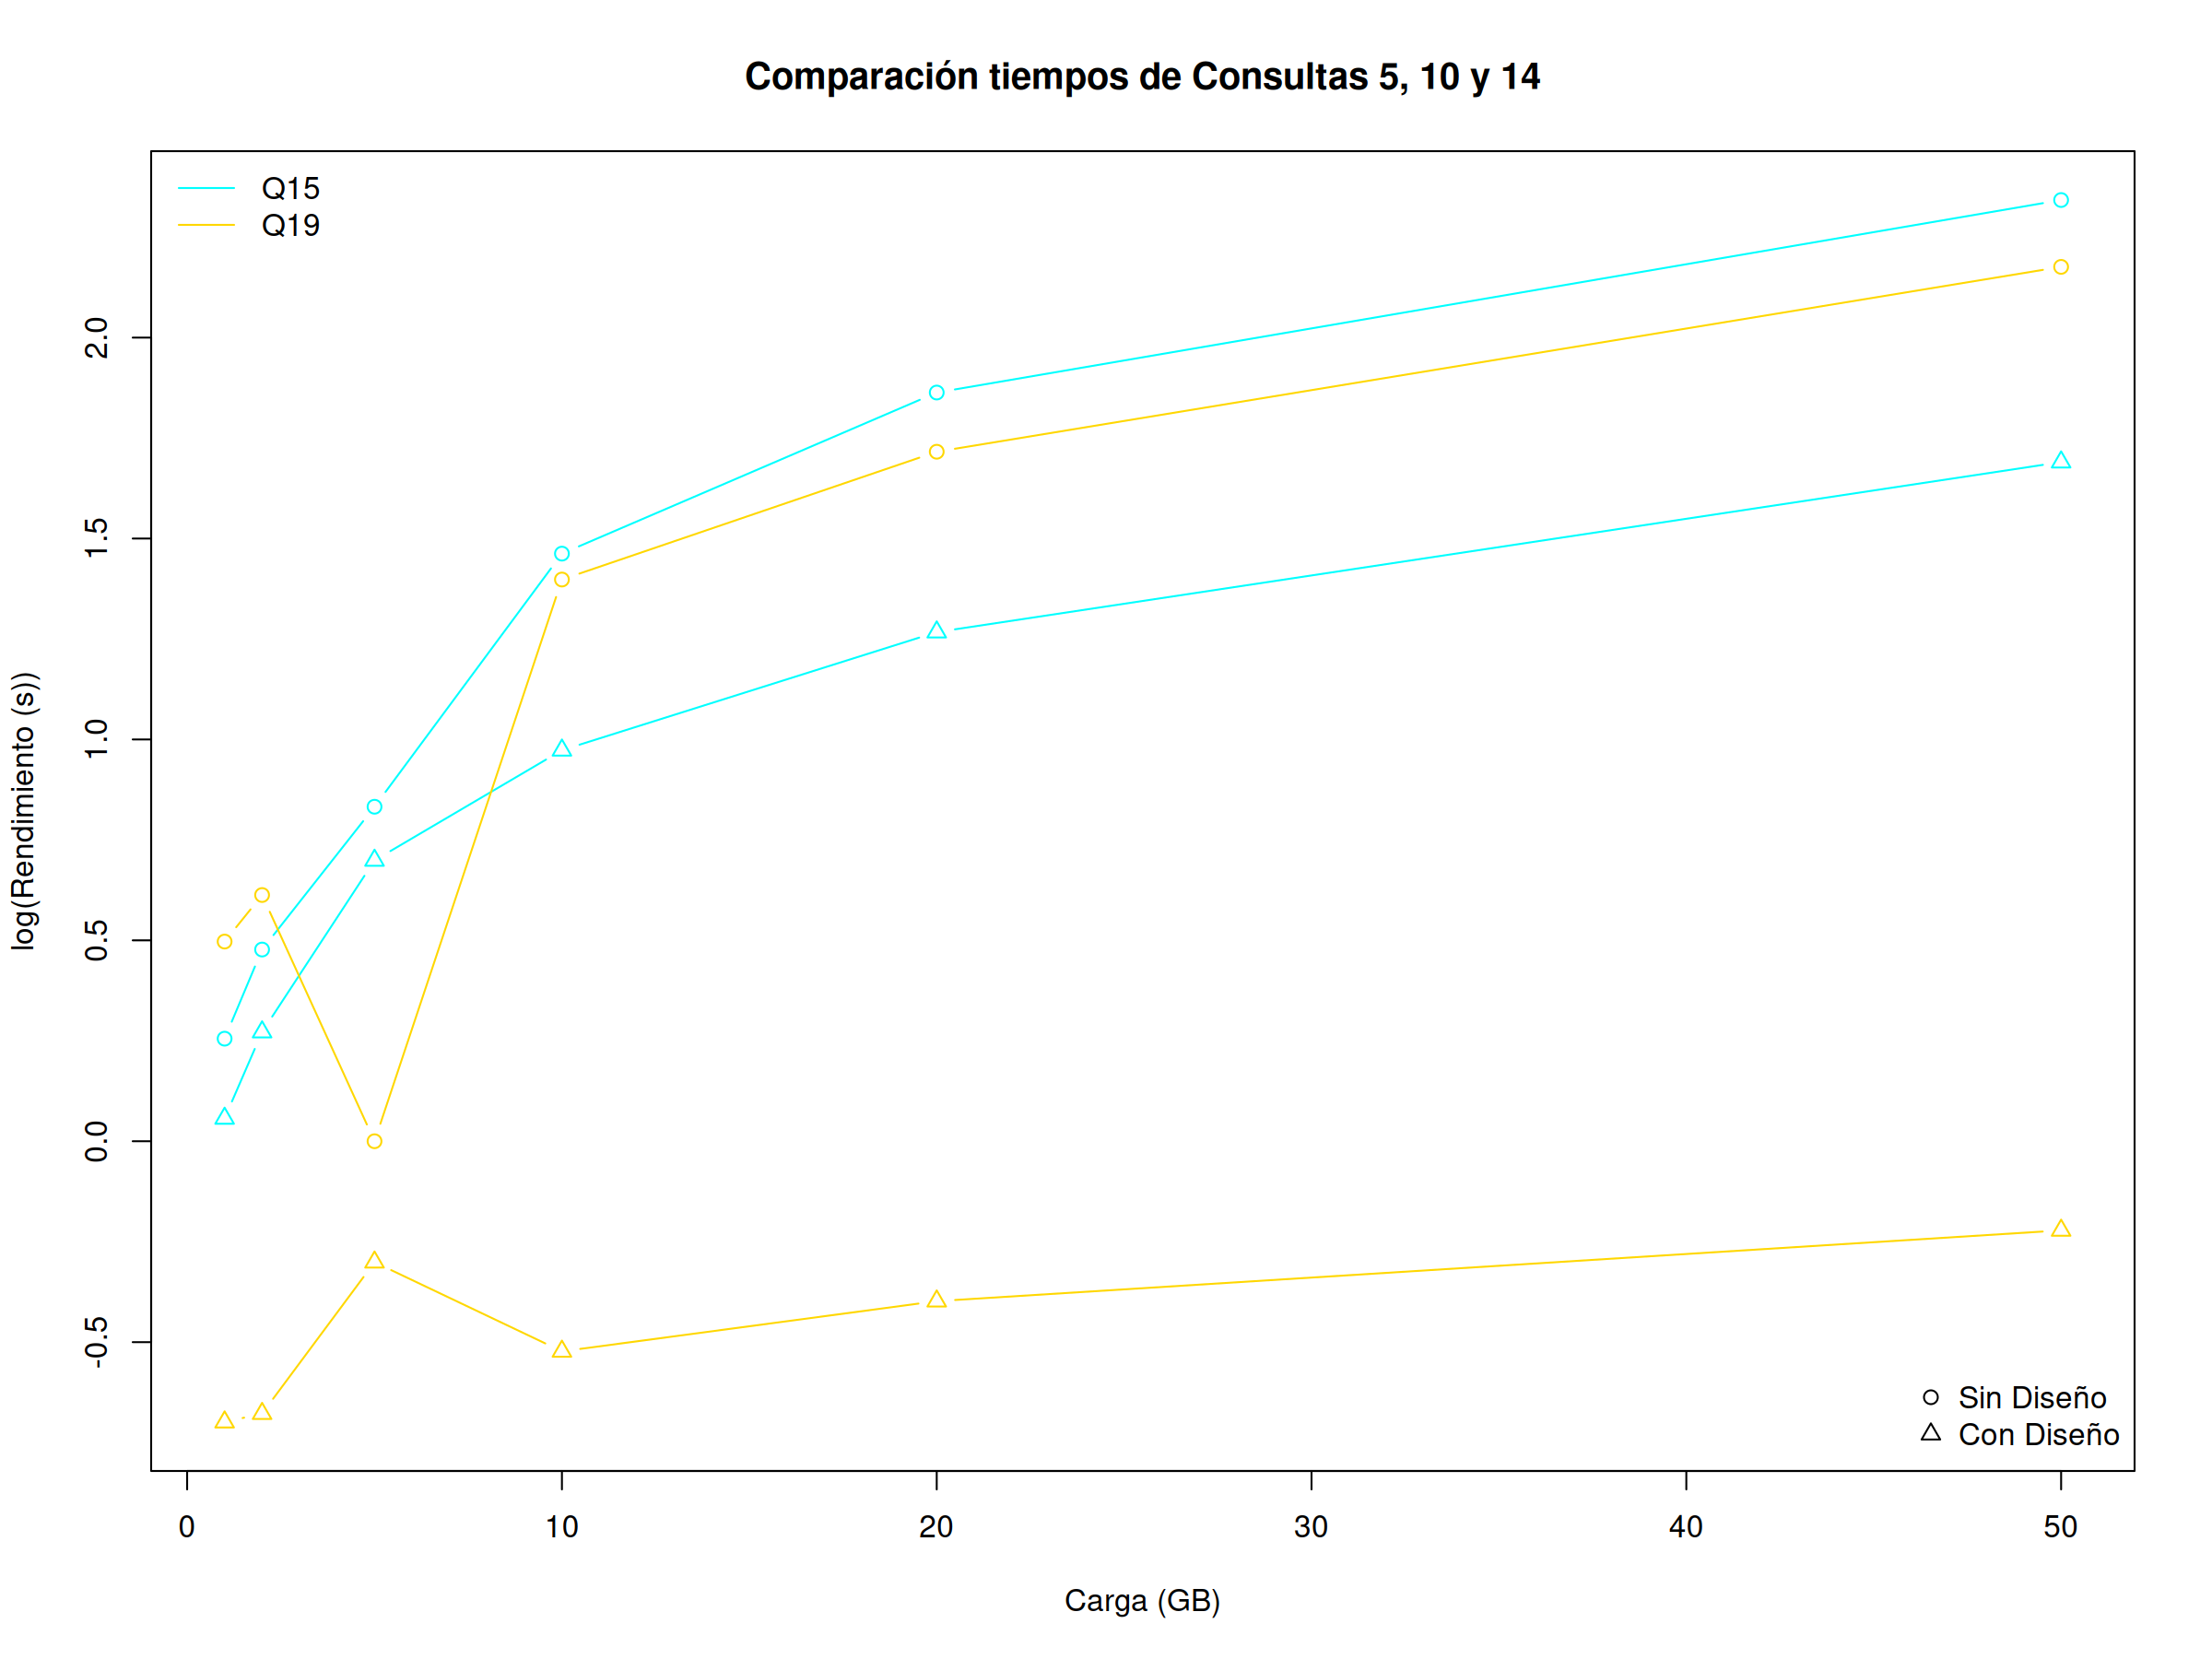
\includegraphics[width = 0.49\textwidth]{images/defensa/tMediaBaja4}
          \caption{Comparación de tiempos consultas intermedias}
        \end{figure}
      \end{frame}

      \begin{frame}{Consultas intermedias}
        \begin{figure}
          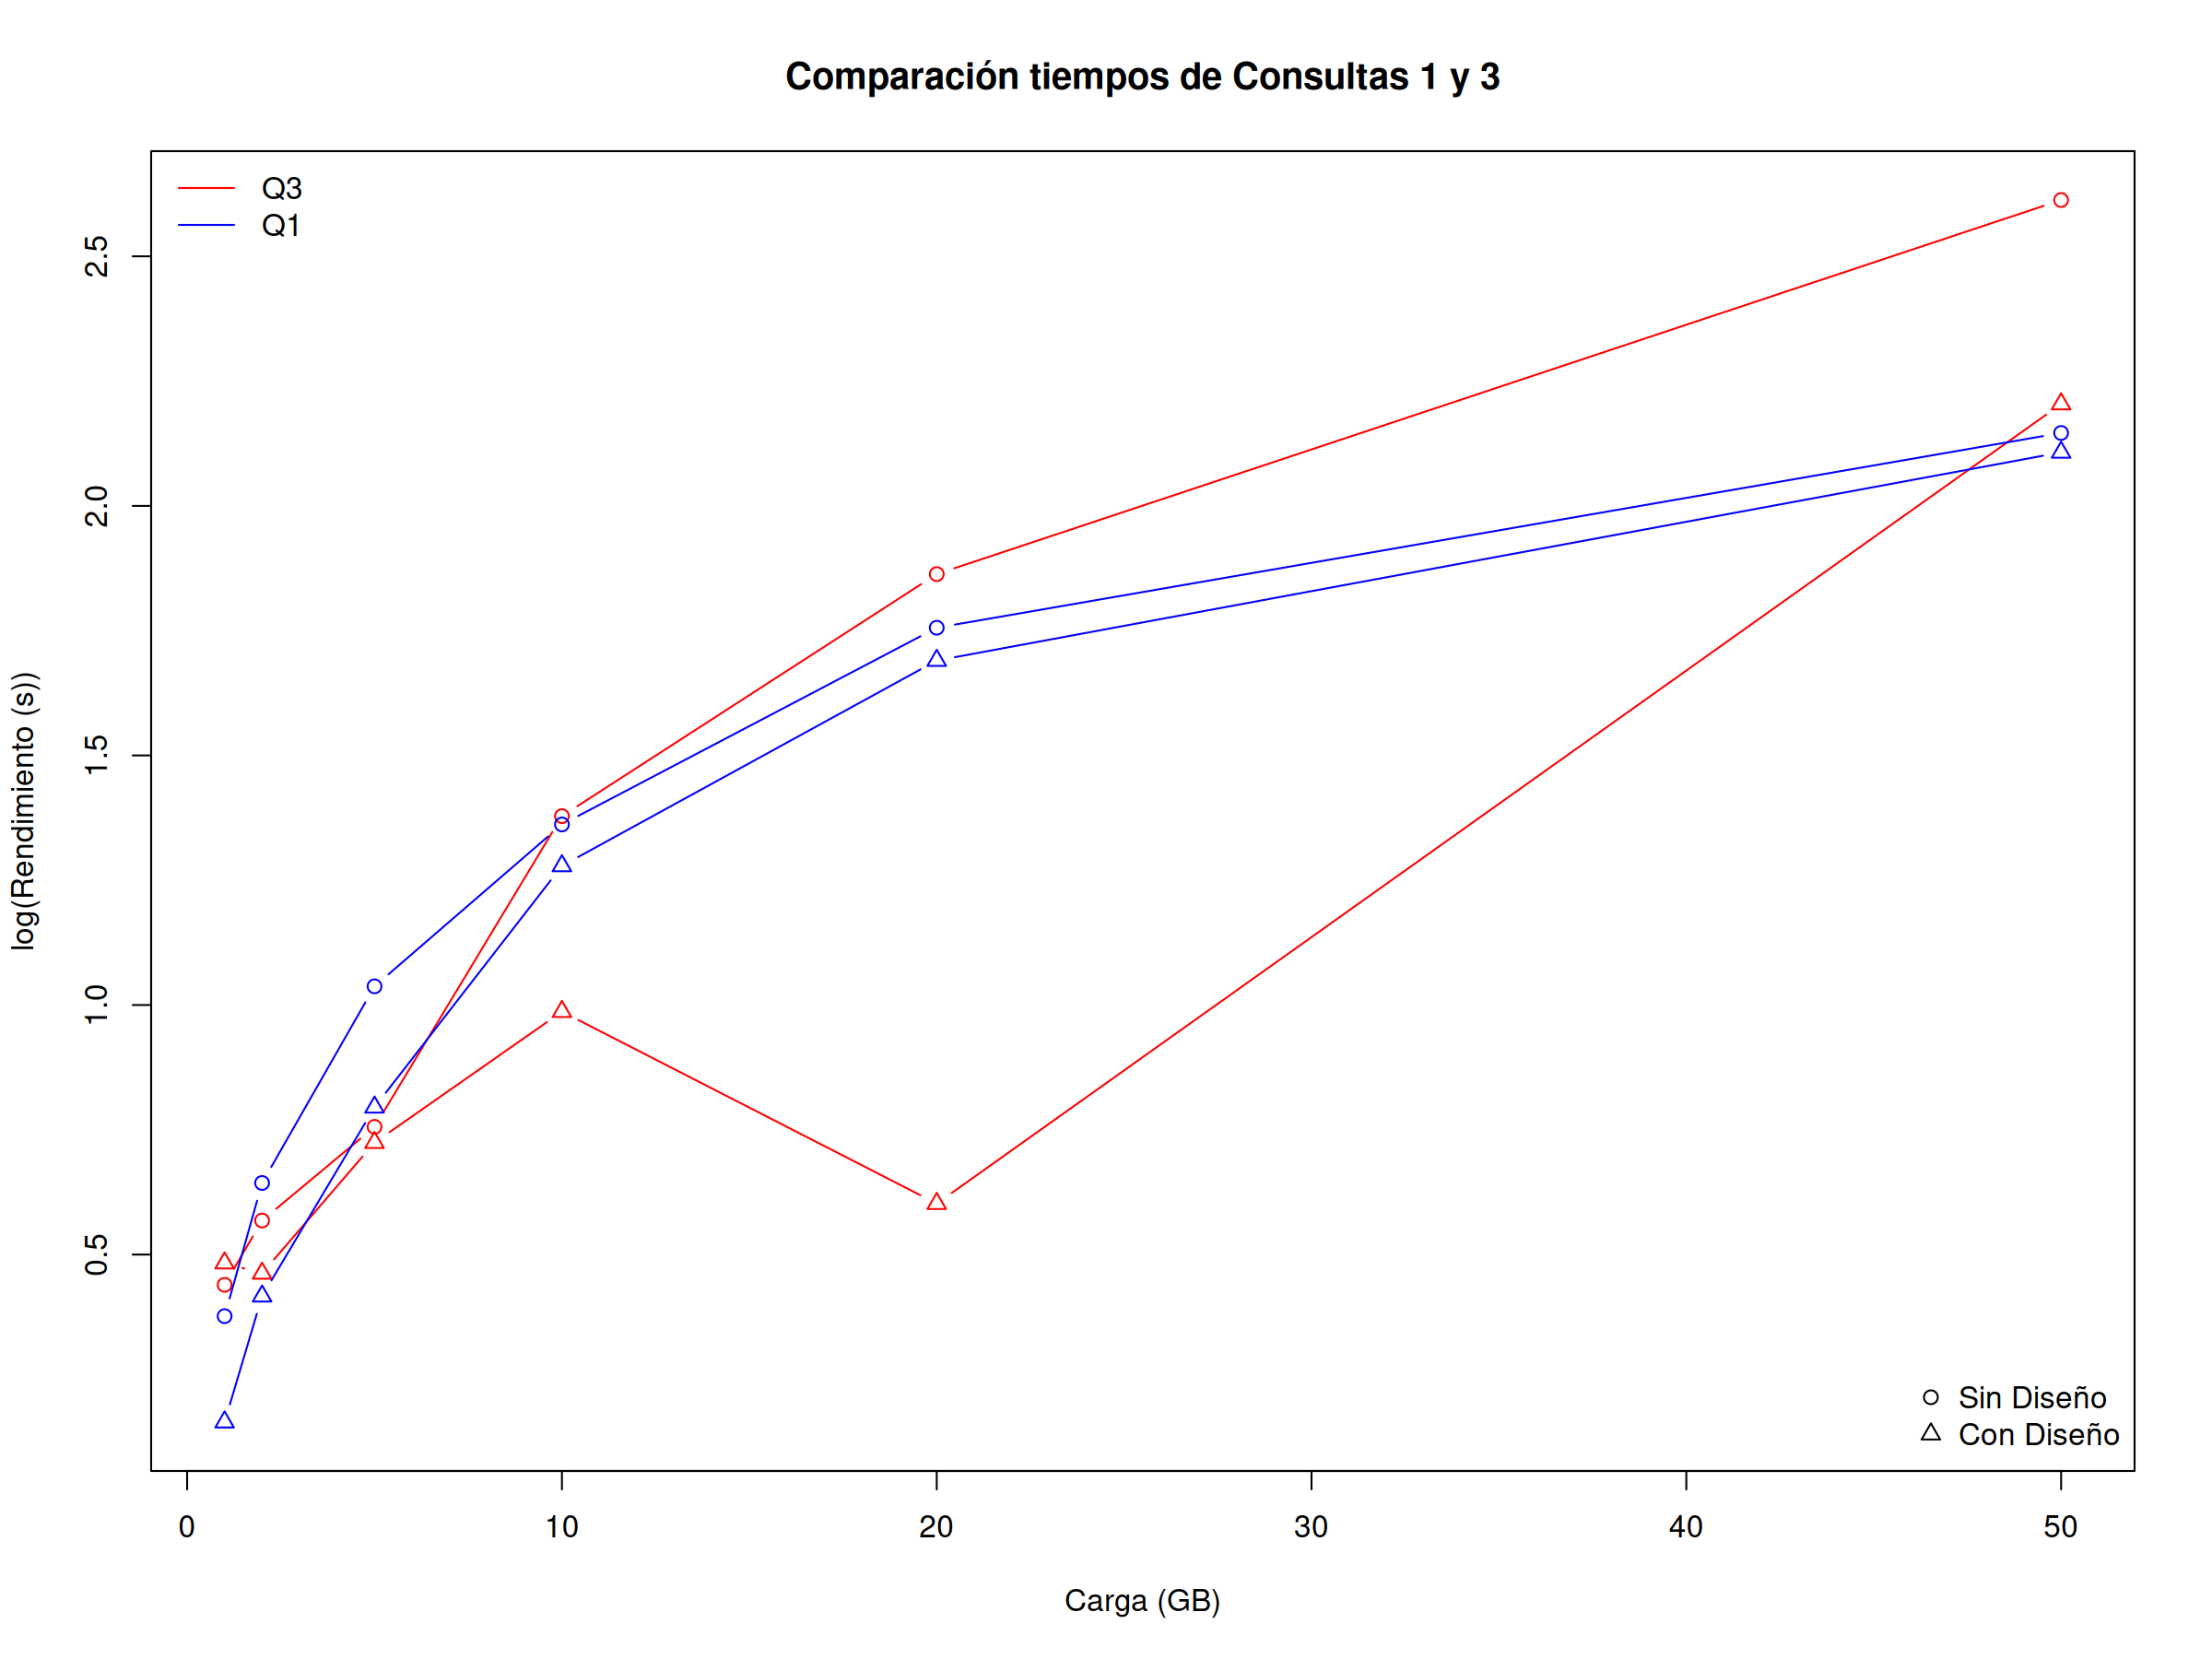
\includegraphics[width = 0.49\textwidth]{images/defensa/tMediaAlta1}
          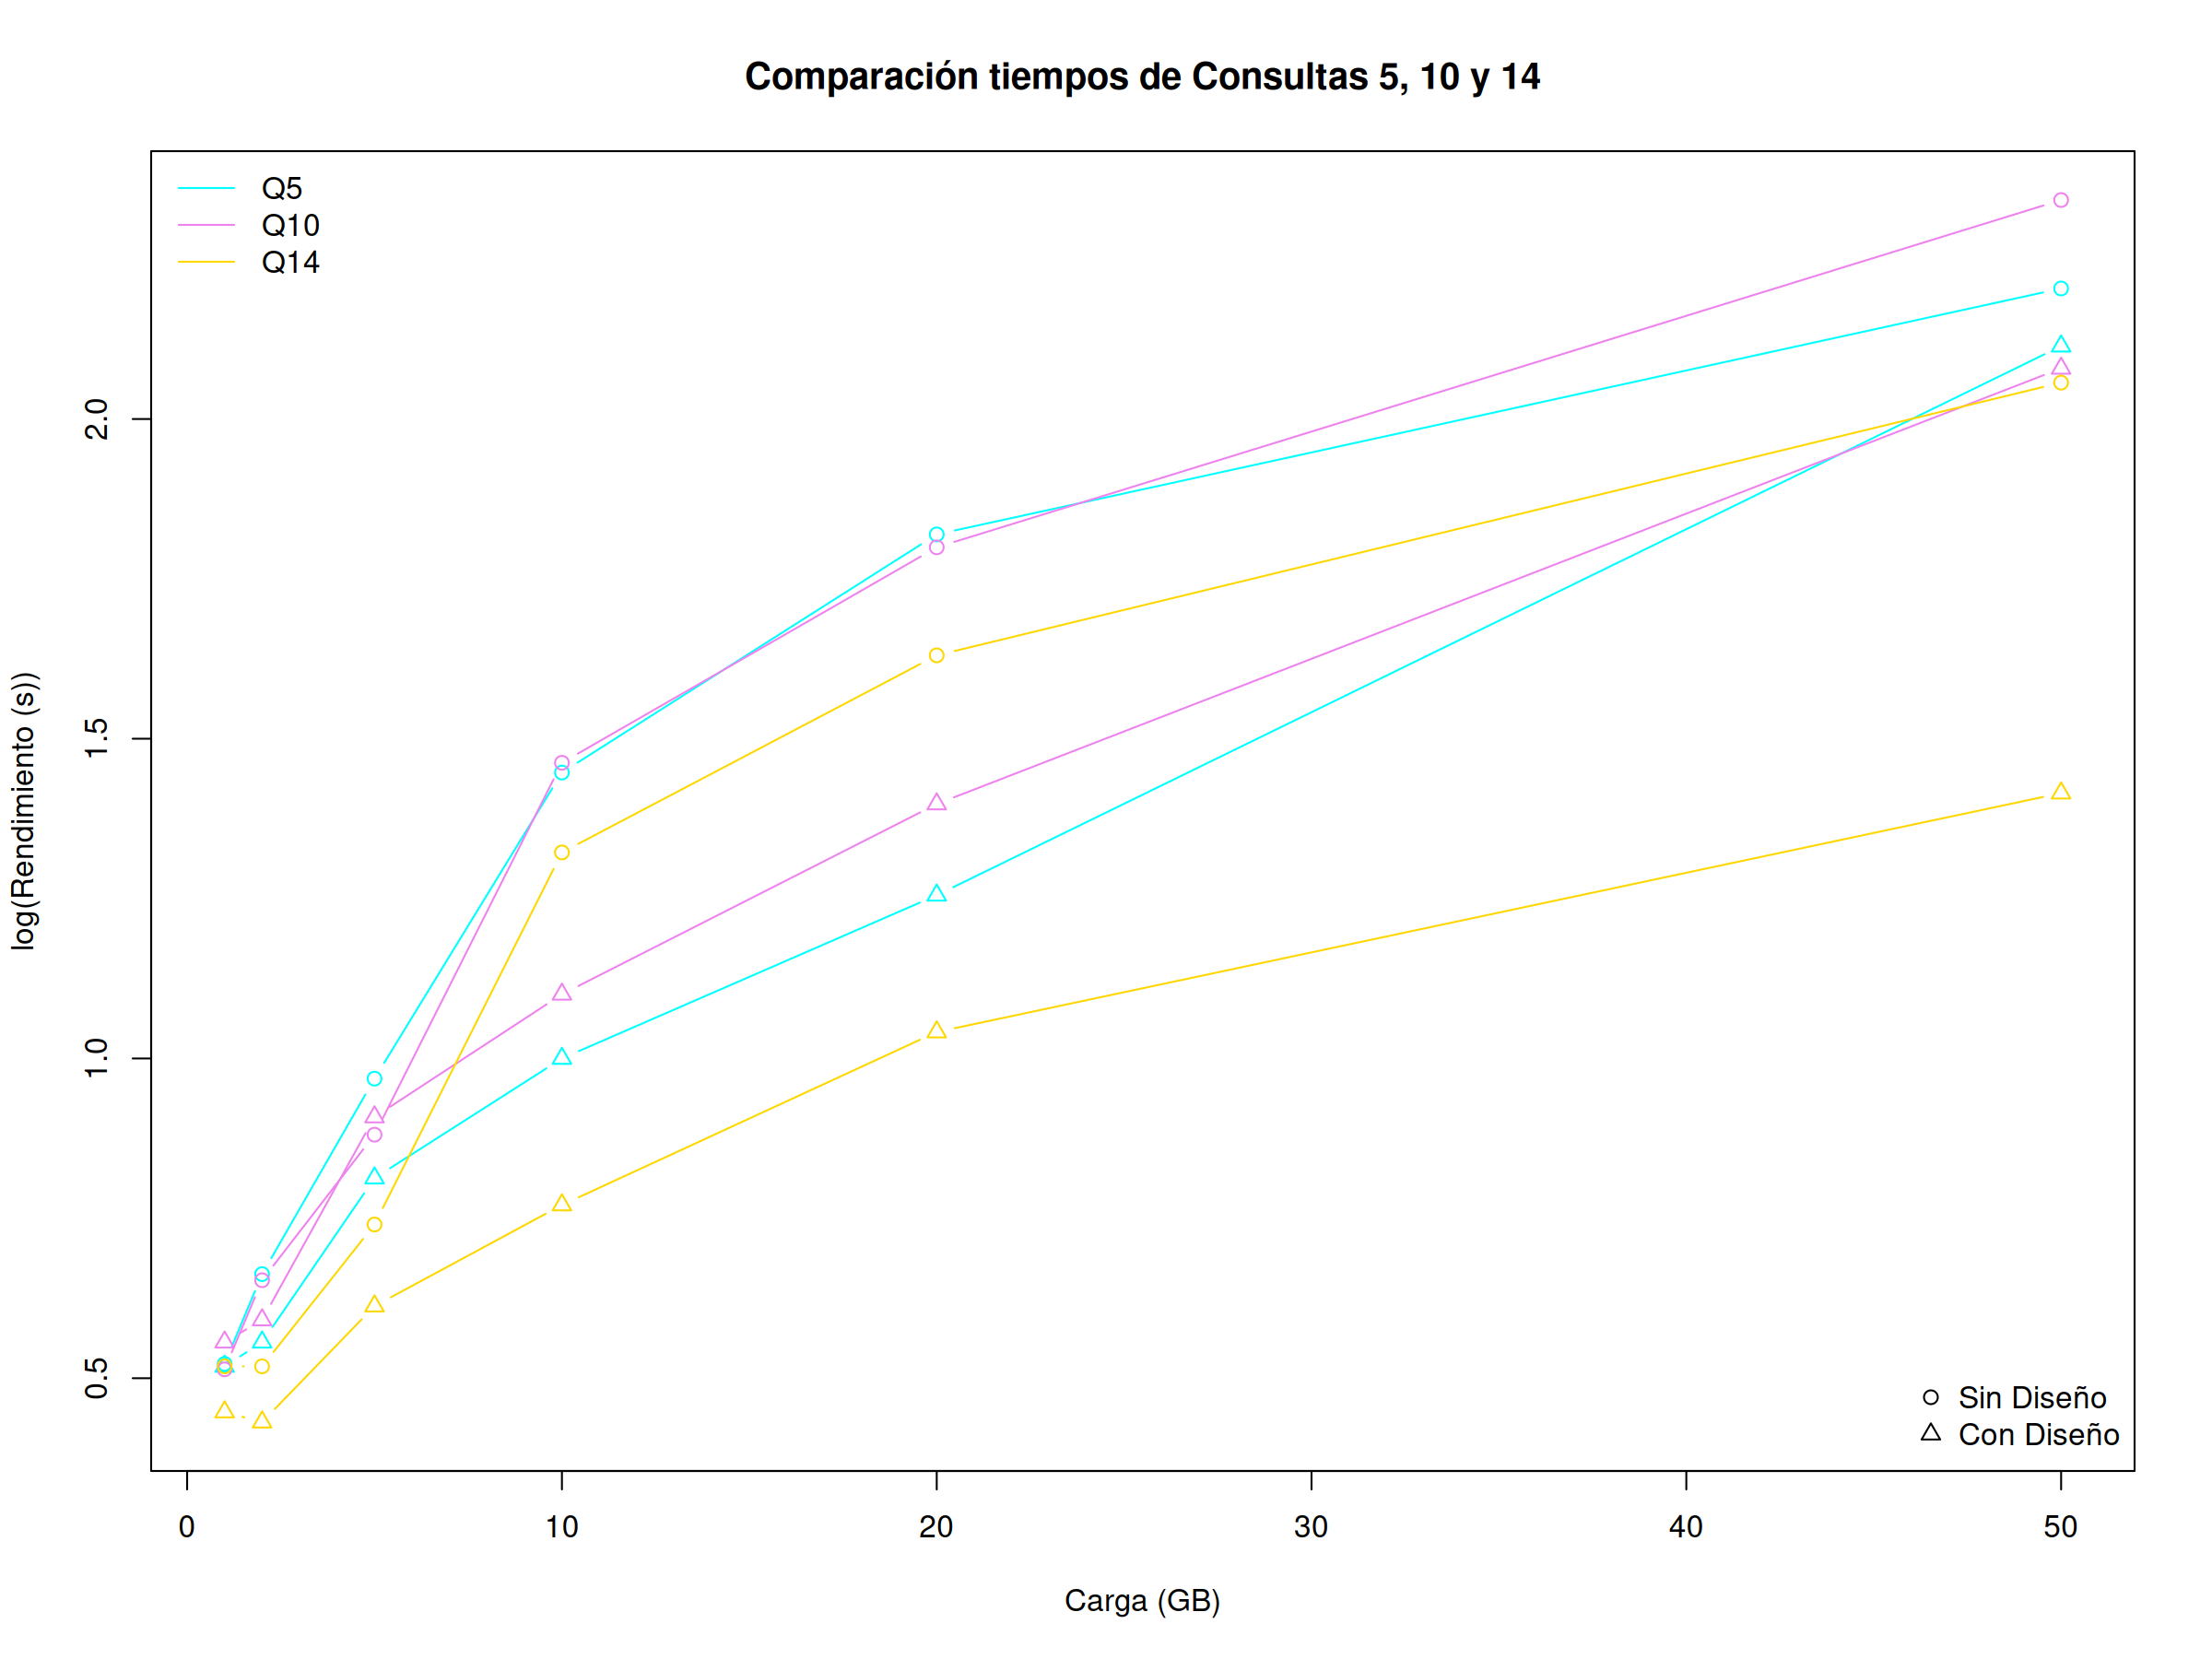
\includegraphics[width = 0.49\textwidth]{images/defensa/tMediaAlta2}
          \caption{Comparación de tiempos consultas intermedias}
        \end{figure}
      \end{frame}

      \begin{frame}{Consultas intermedias}
        \begin{figure}
          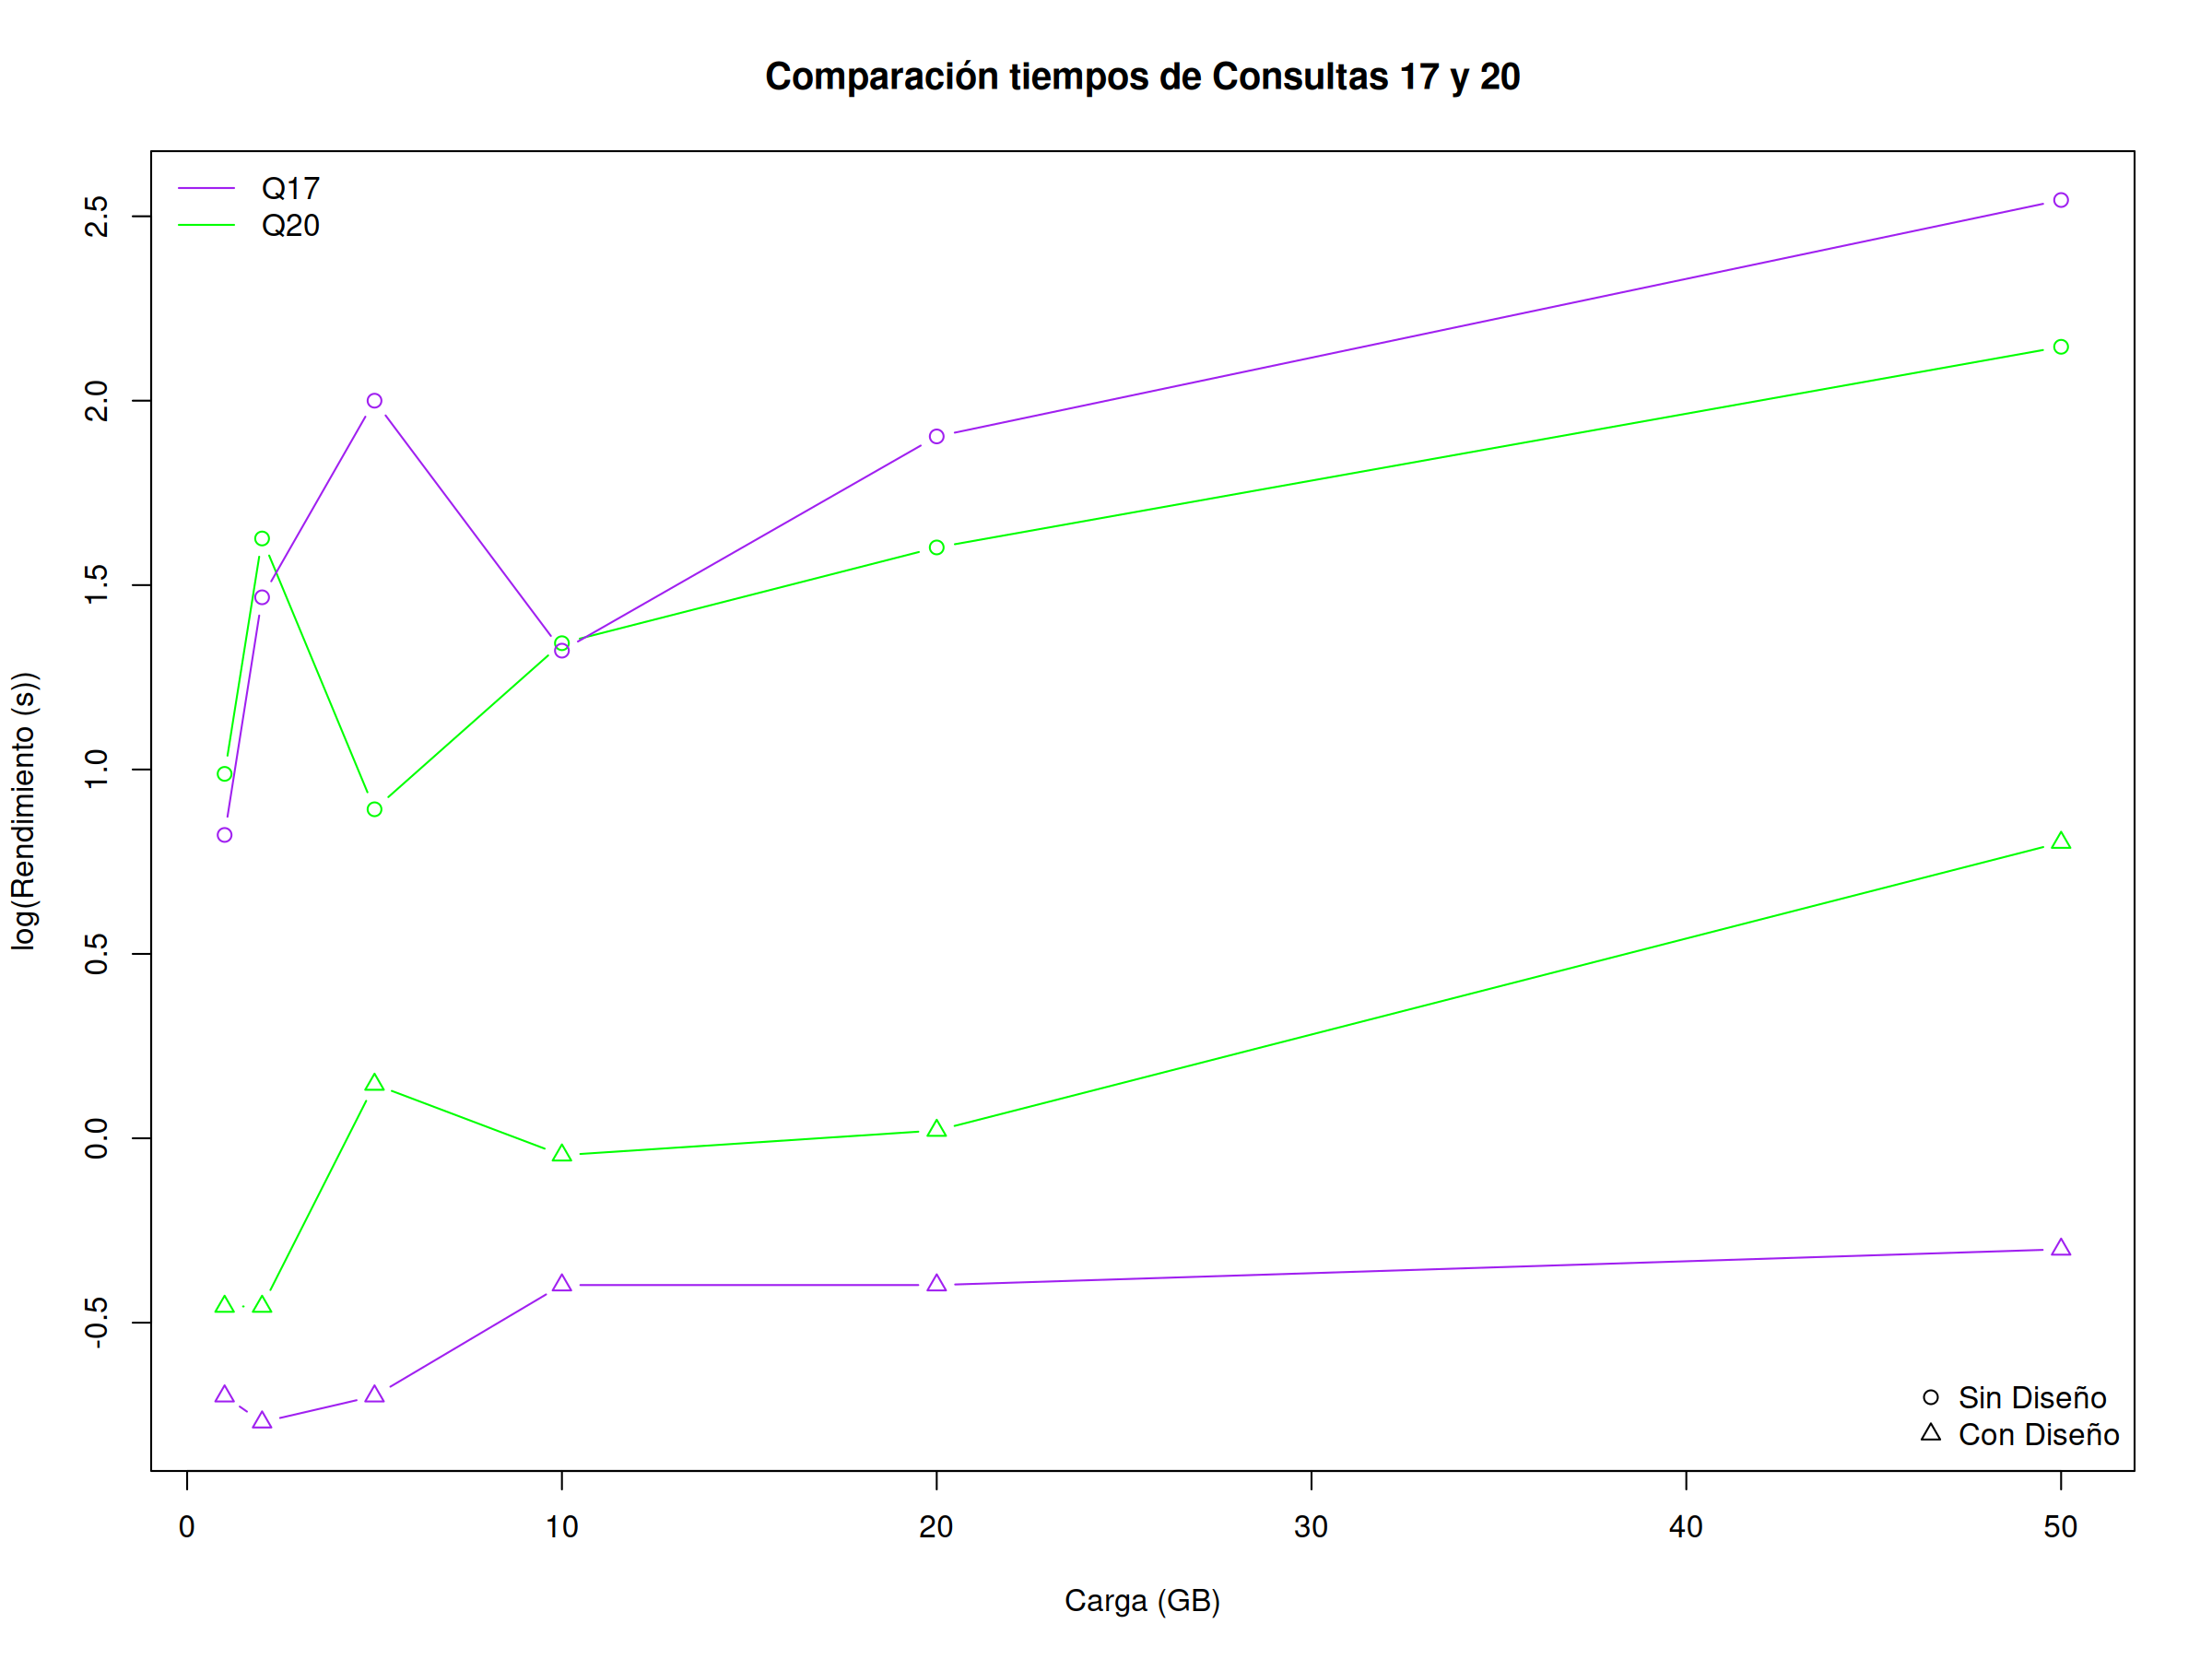
\includegraphics[width = 0.75\textwidth]{images/defensa/tMediaAlta3}
          \caption{Comparación de tiempos consultas intermedias}
        \end{figure}
      \end{frame}

      \begin{frame}{Consultas pesadas}
        \begin{figure}
          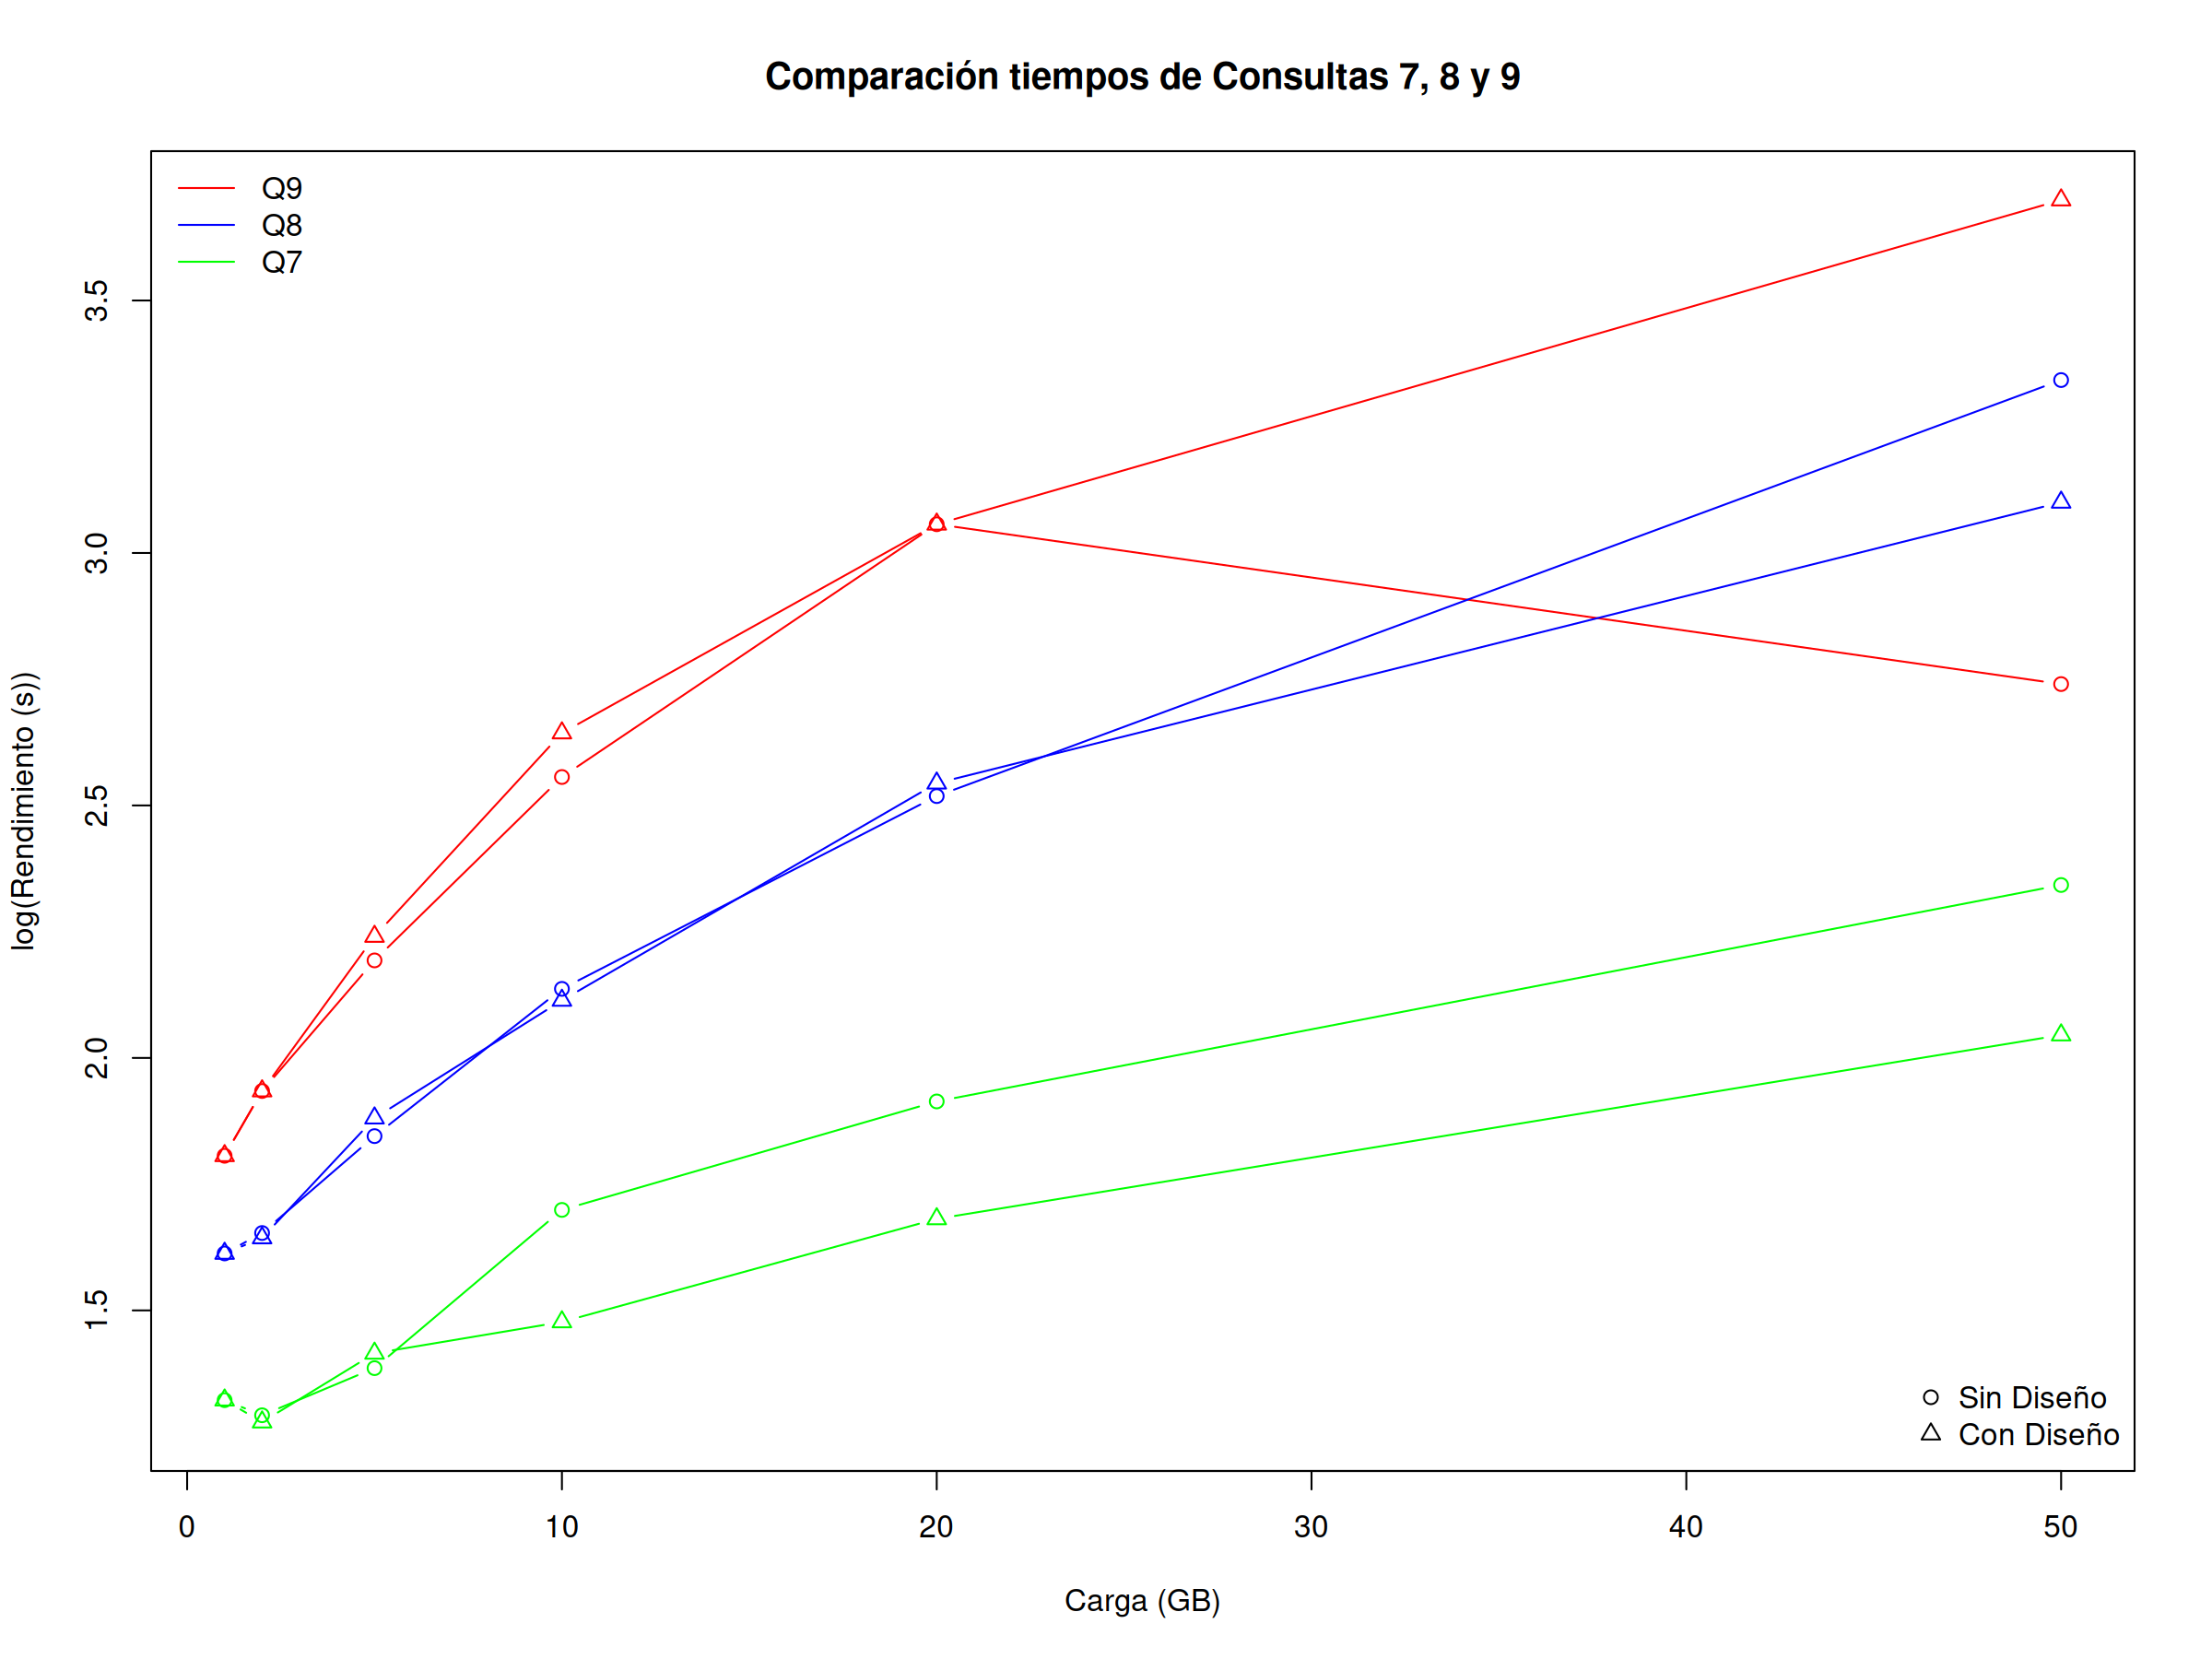
\includegraphics[width = 0.75\textwidth]{images/defensa/tPesadas.png}
          \caption{Comparación de tiempos consultas pesadas}
        \end{figure}
      \end{frame}

      \begin{frame}{Comparación global por cargas}
        \begin{figure}
          
\includegraphics[width = 0.49\textwidth]{images/Tiempo-1G.png}
          
\includegraphics[width = 0.49\textwidth]{images/Tiempo-2G.png}
          \caption{Tiempo por consulta 1 GB (izquierda) y 2 GB (derecha)}
        \end{figure}
      \end{frame}

      \begin{frame}{Comparación global por cargas}
        \begin{figure}
          
\includegraphics[width = 0.49\textwidth]{images/Tiempo-5G.png}
          
\includegraphics[width = 0.49\textwidth]{images/Tiempo-10G.png}
          \caption{Tiempo por consulta 5 GB (izquierda) y 10 GB (derecha)}
        \end{figure}
      \end{frame}

      \begin{frame}{Comparación global por cargas}
        \begin{figure}
          
\includegraphics[width = 0.49\textwidth]{images/Tiempo-20G.png}
          
\includegraphics[width = 0.49\textwidth]{images/Tiempo-50G.png}
          \caption{Tiempo por consulta 20 GB (izquierda) y 50 GB (derecha)}
        \end{figure}
      \end{frame}

      \begin{frame}{Resumen de impacto de la estrategia sobre el rendimiento}
        \begin{figure}
          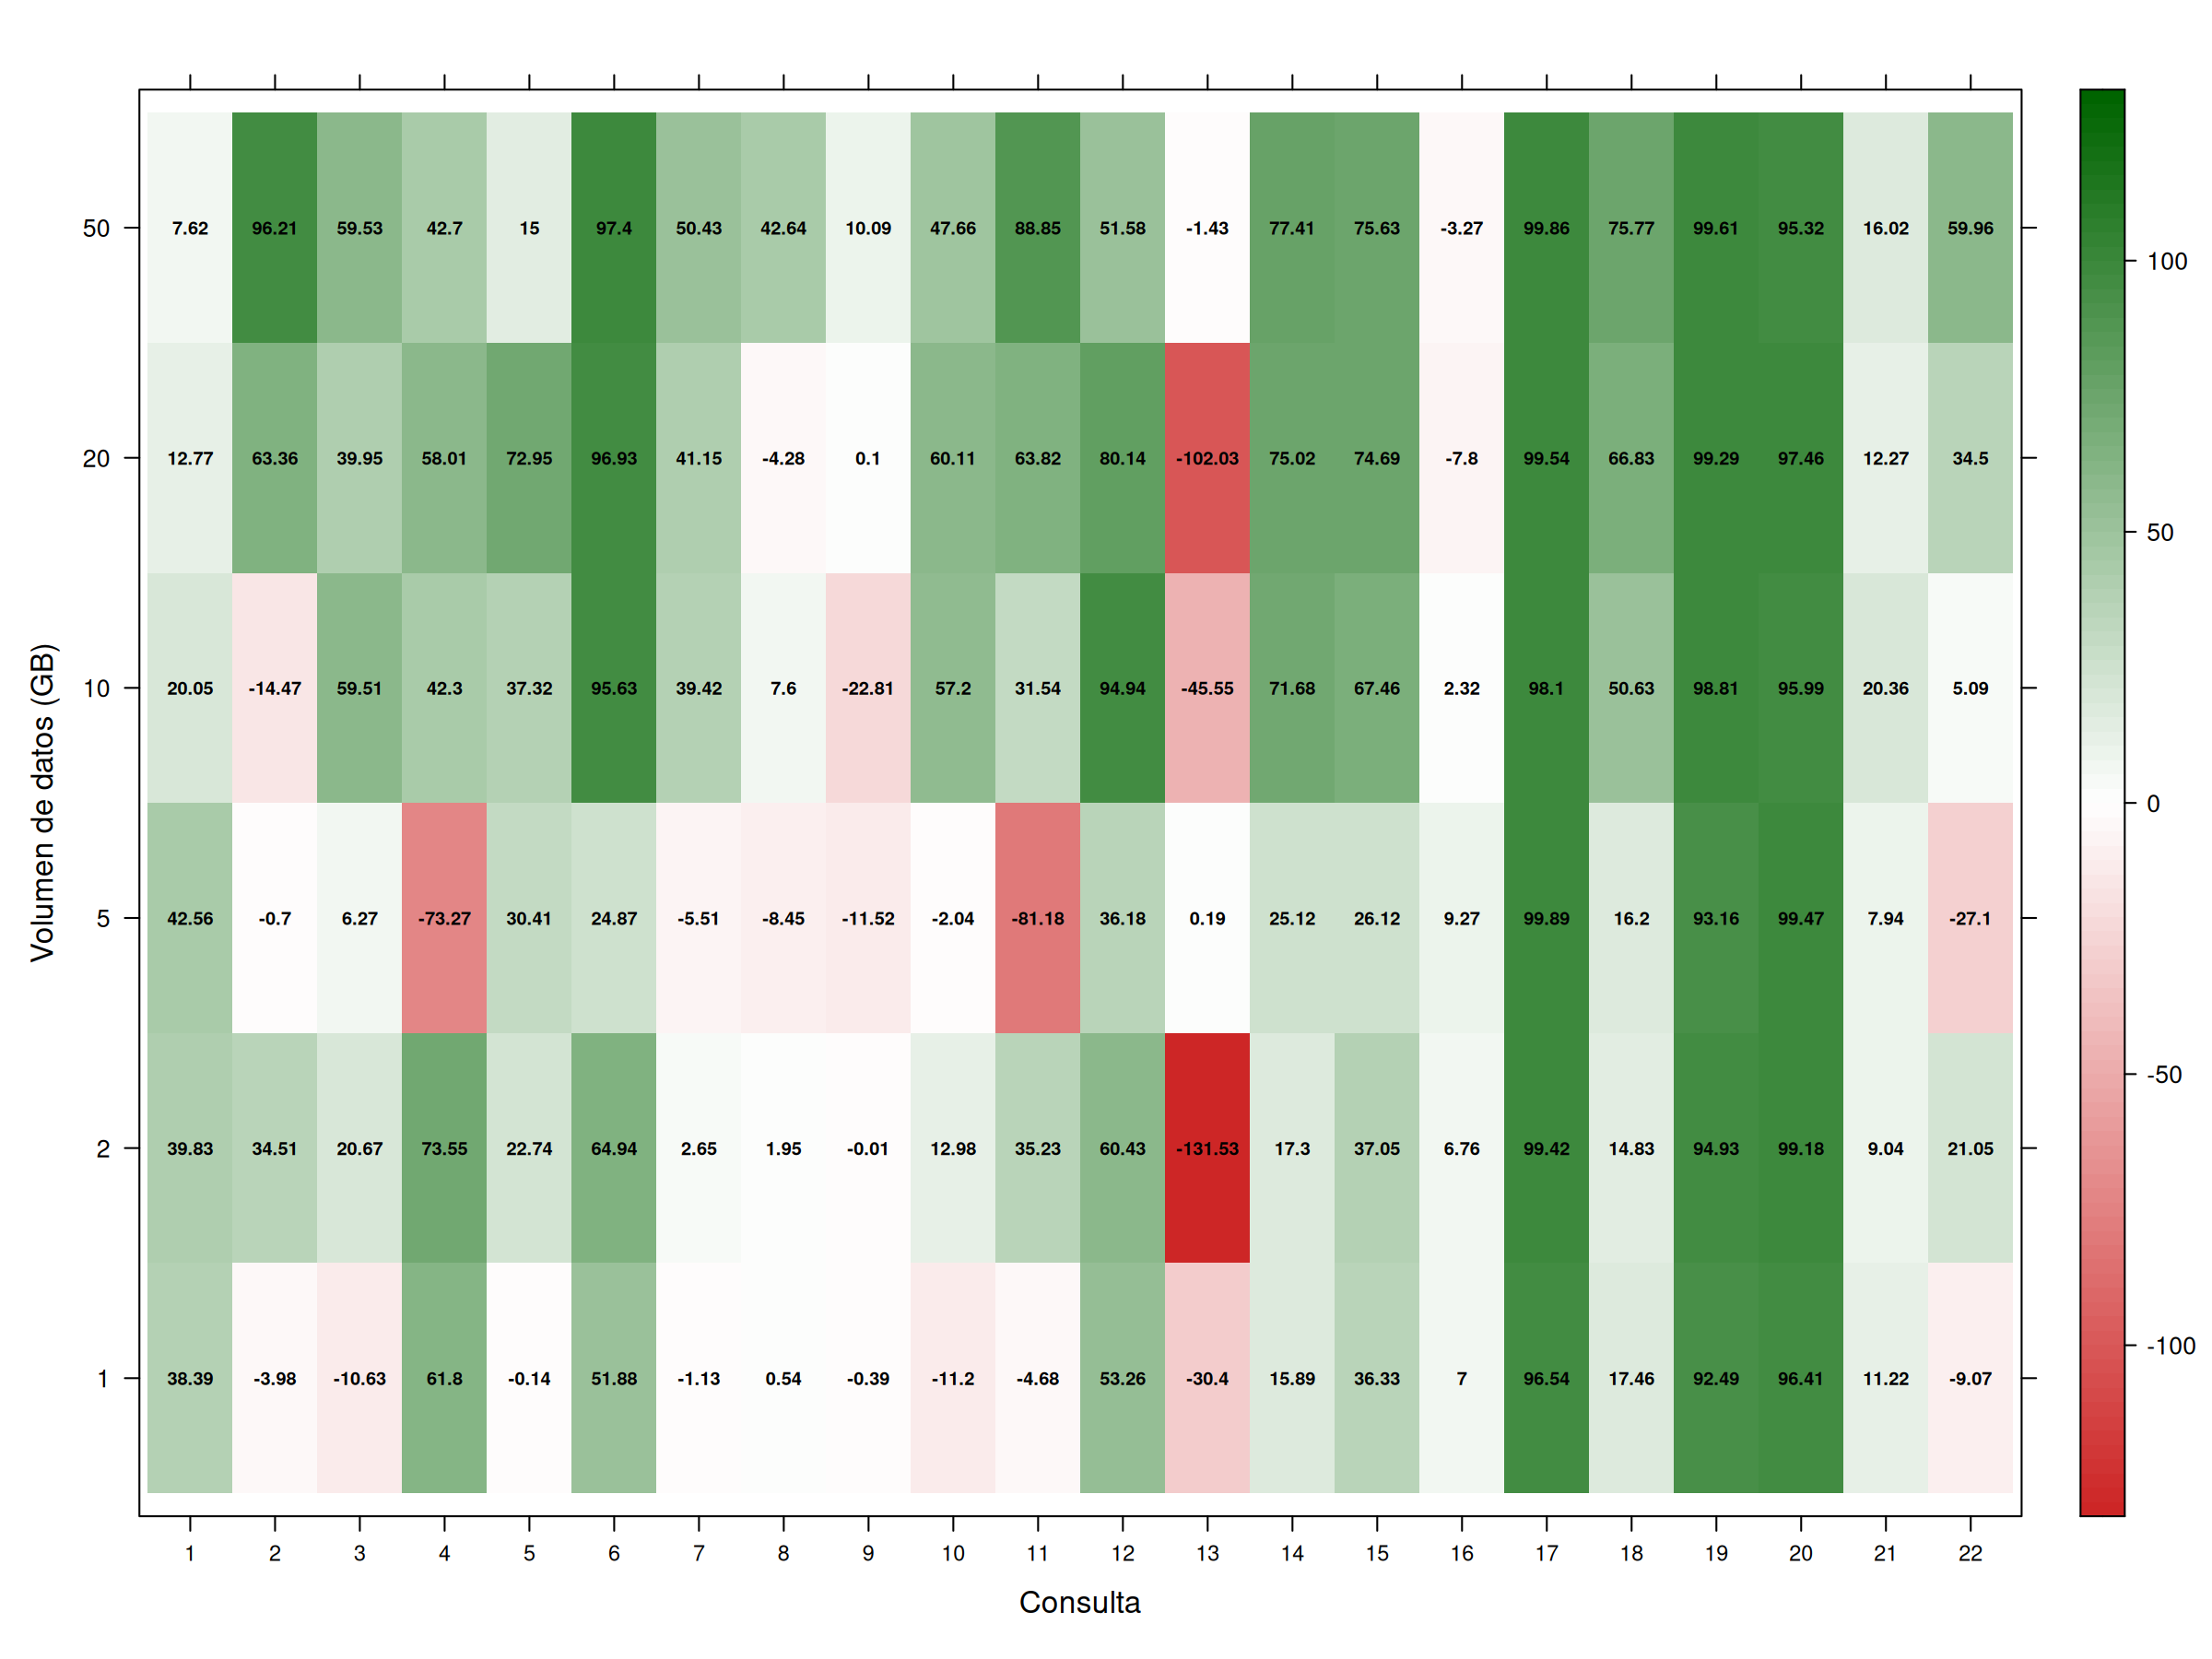
\includegraphics[width = 0.75\textwidth]{images/mejorasT.png}
          \caption{Mapa de calor de mejoras en rendimiento de las consultas}
        \end{figure}
      \end{frame}
    % subsection rendimiento (end)

    \subsection{Consumo neto} % (fold)
    \label{sub:consumo_neto}
      \begin{frame}{Consumo mínimo}
        \begin{figure}
          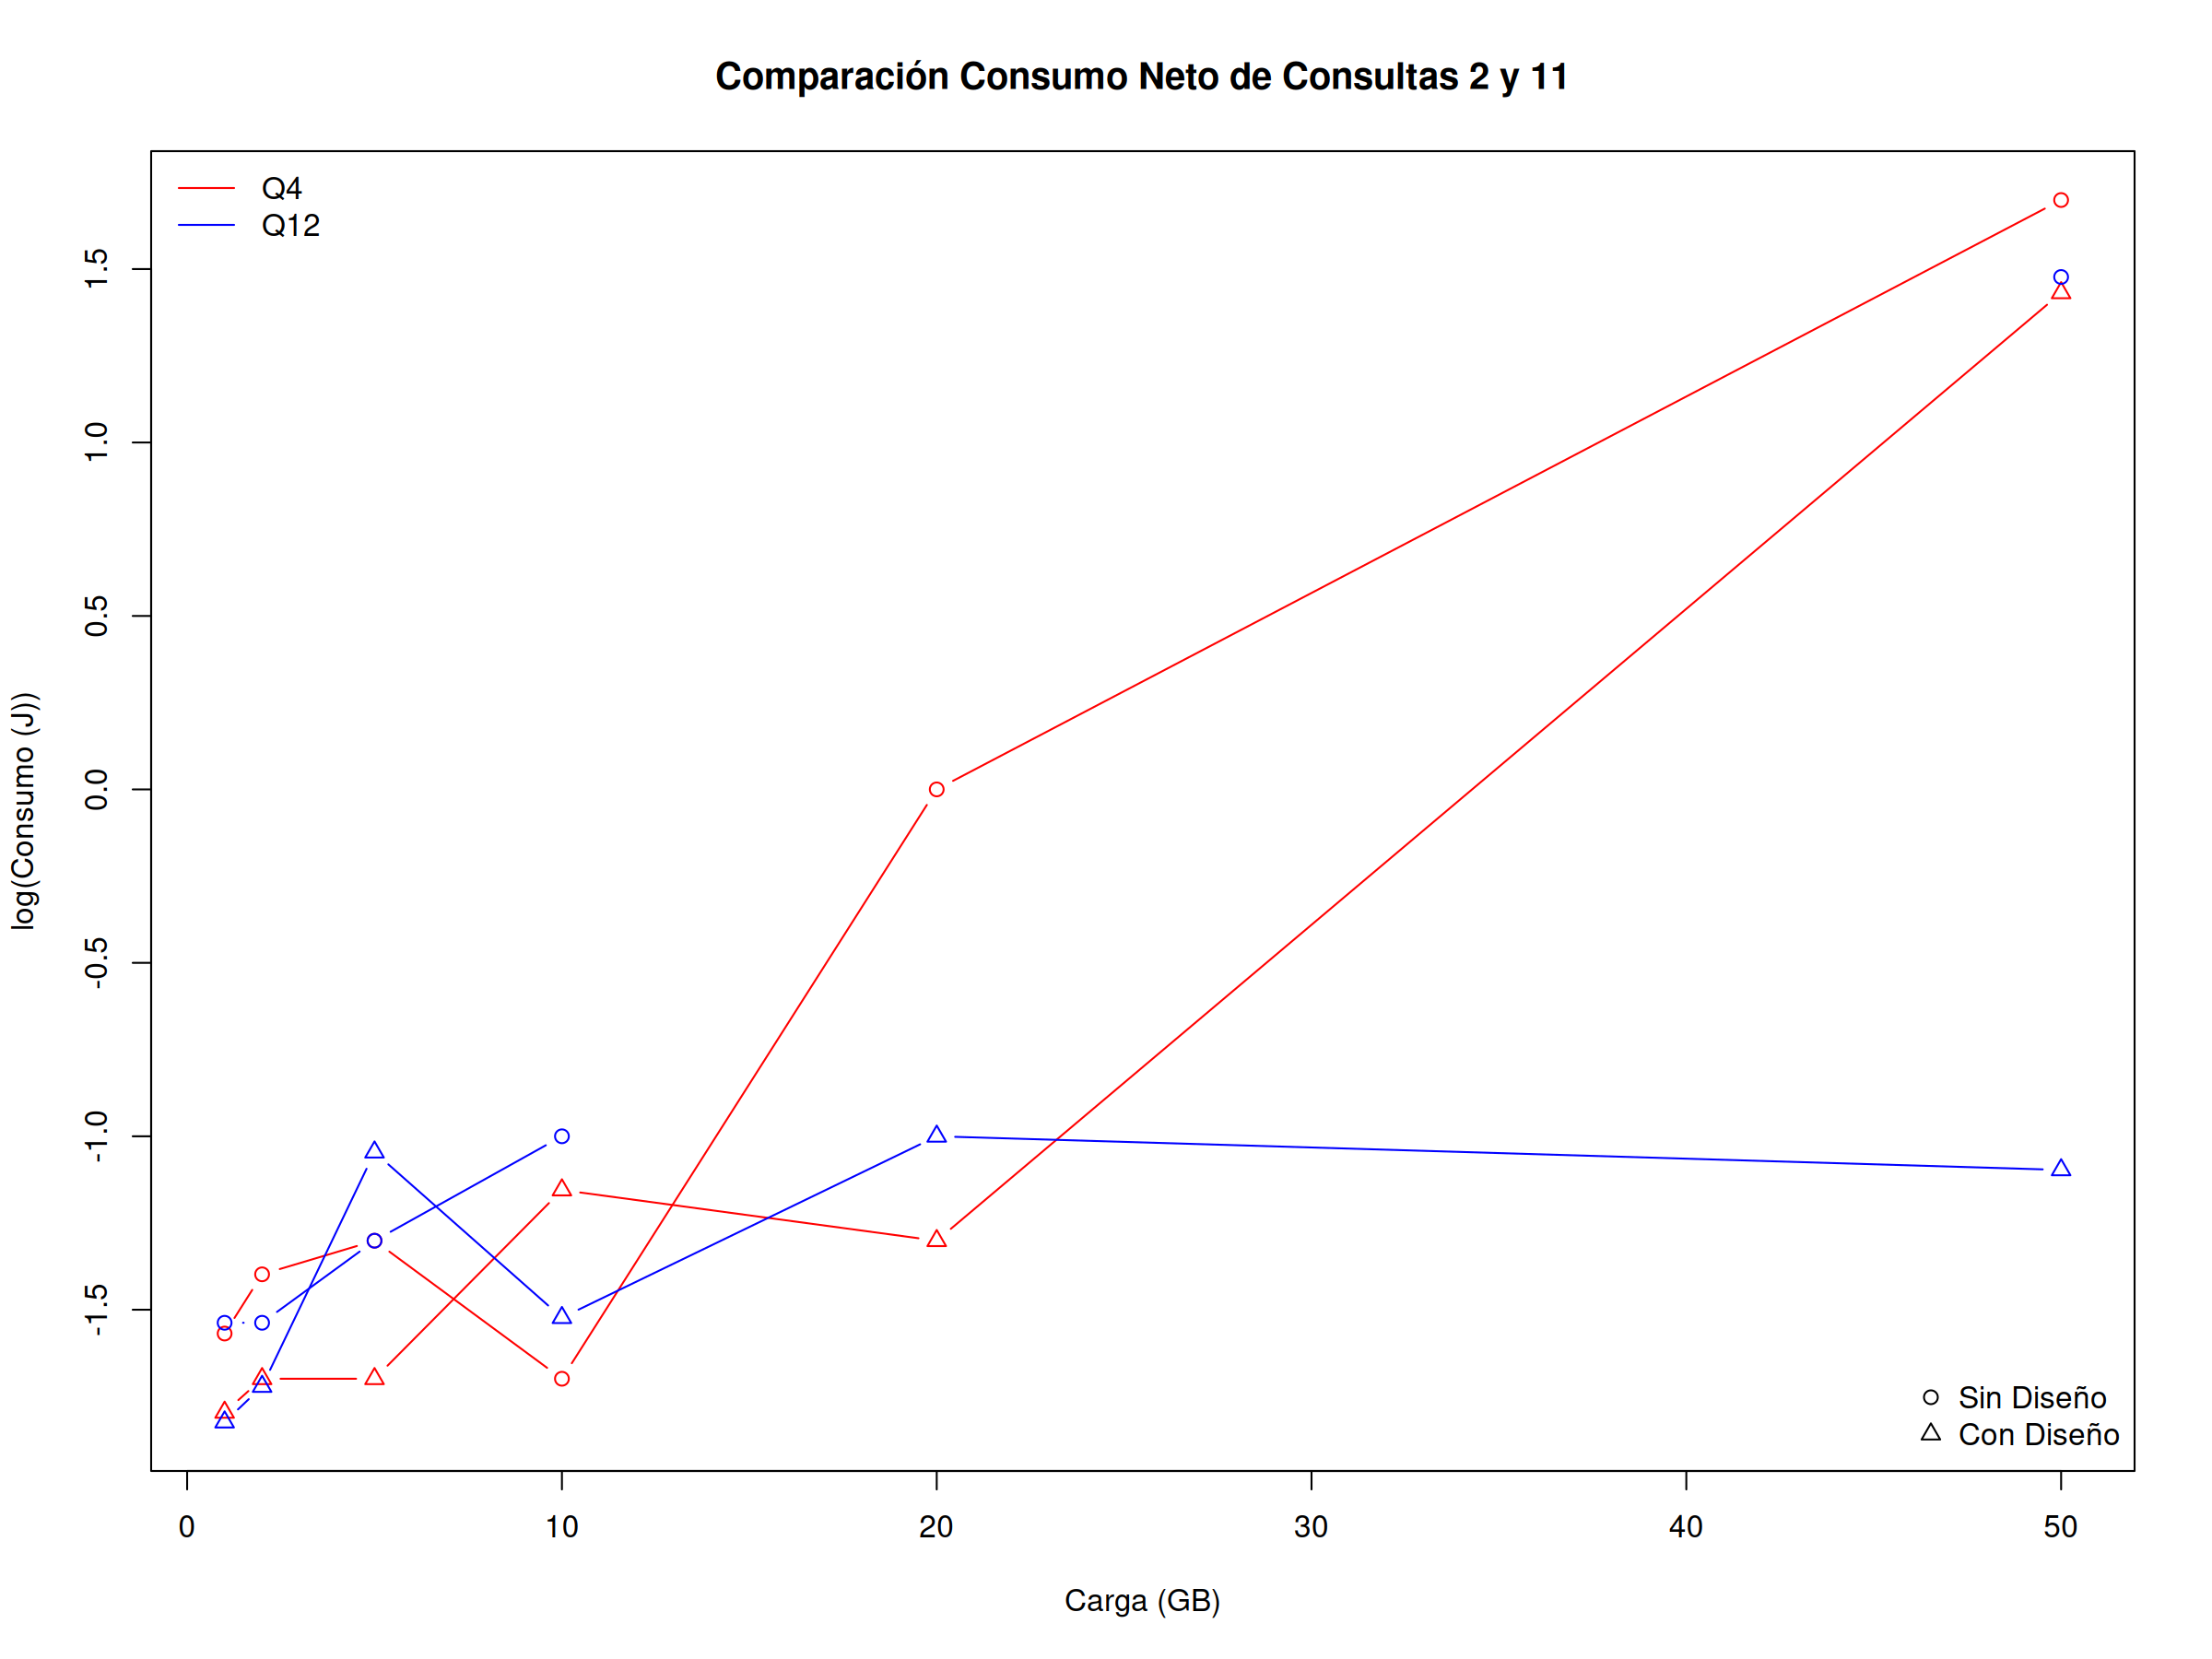
\includegraphics[width = 0.49\textwidth]{images/defensa/cMuyBajo1.png}
          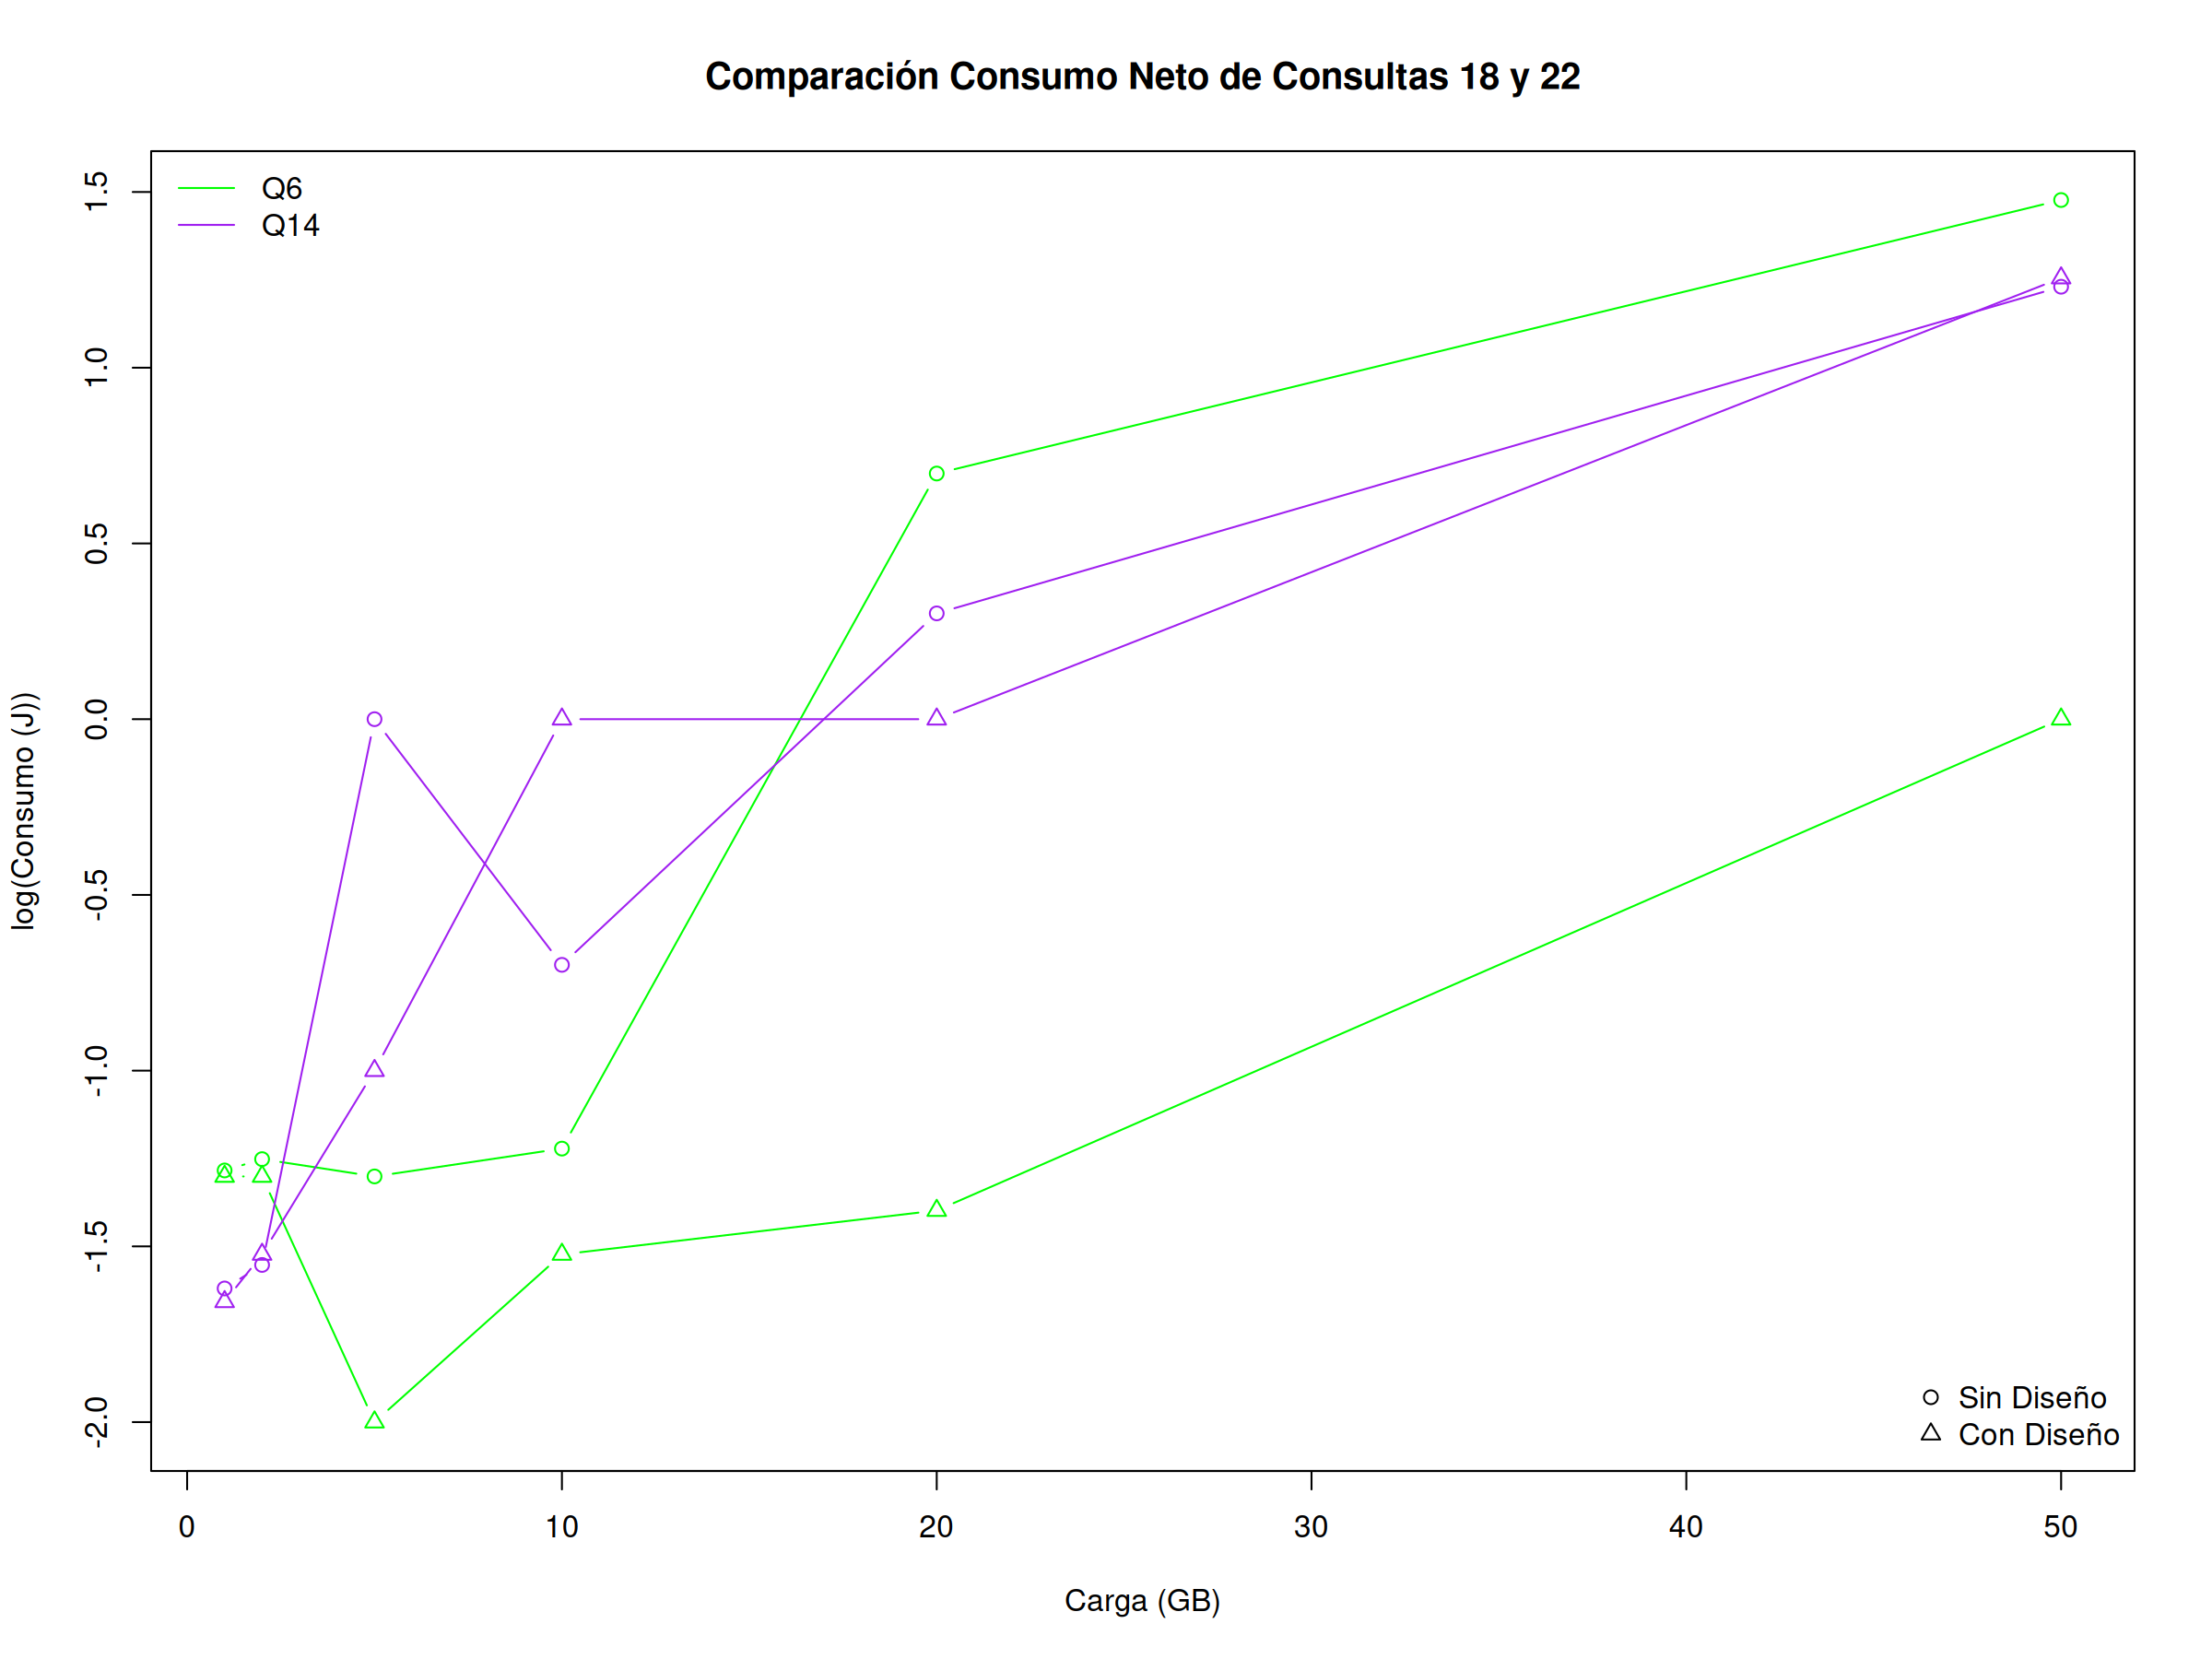
\includegraphics[width = 0.49\textwidth]{images/defensa/cMuyBajo2.png}
          \caption{Comparación de consultas: consumo neto (mínimo)}
        \end{figure}
      \end{frame}

      \begin{frame}{Consumo bajo}
        \begin{figure}
          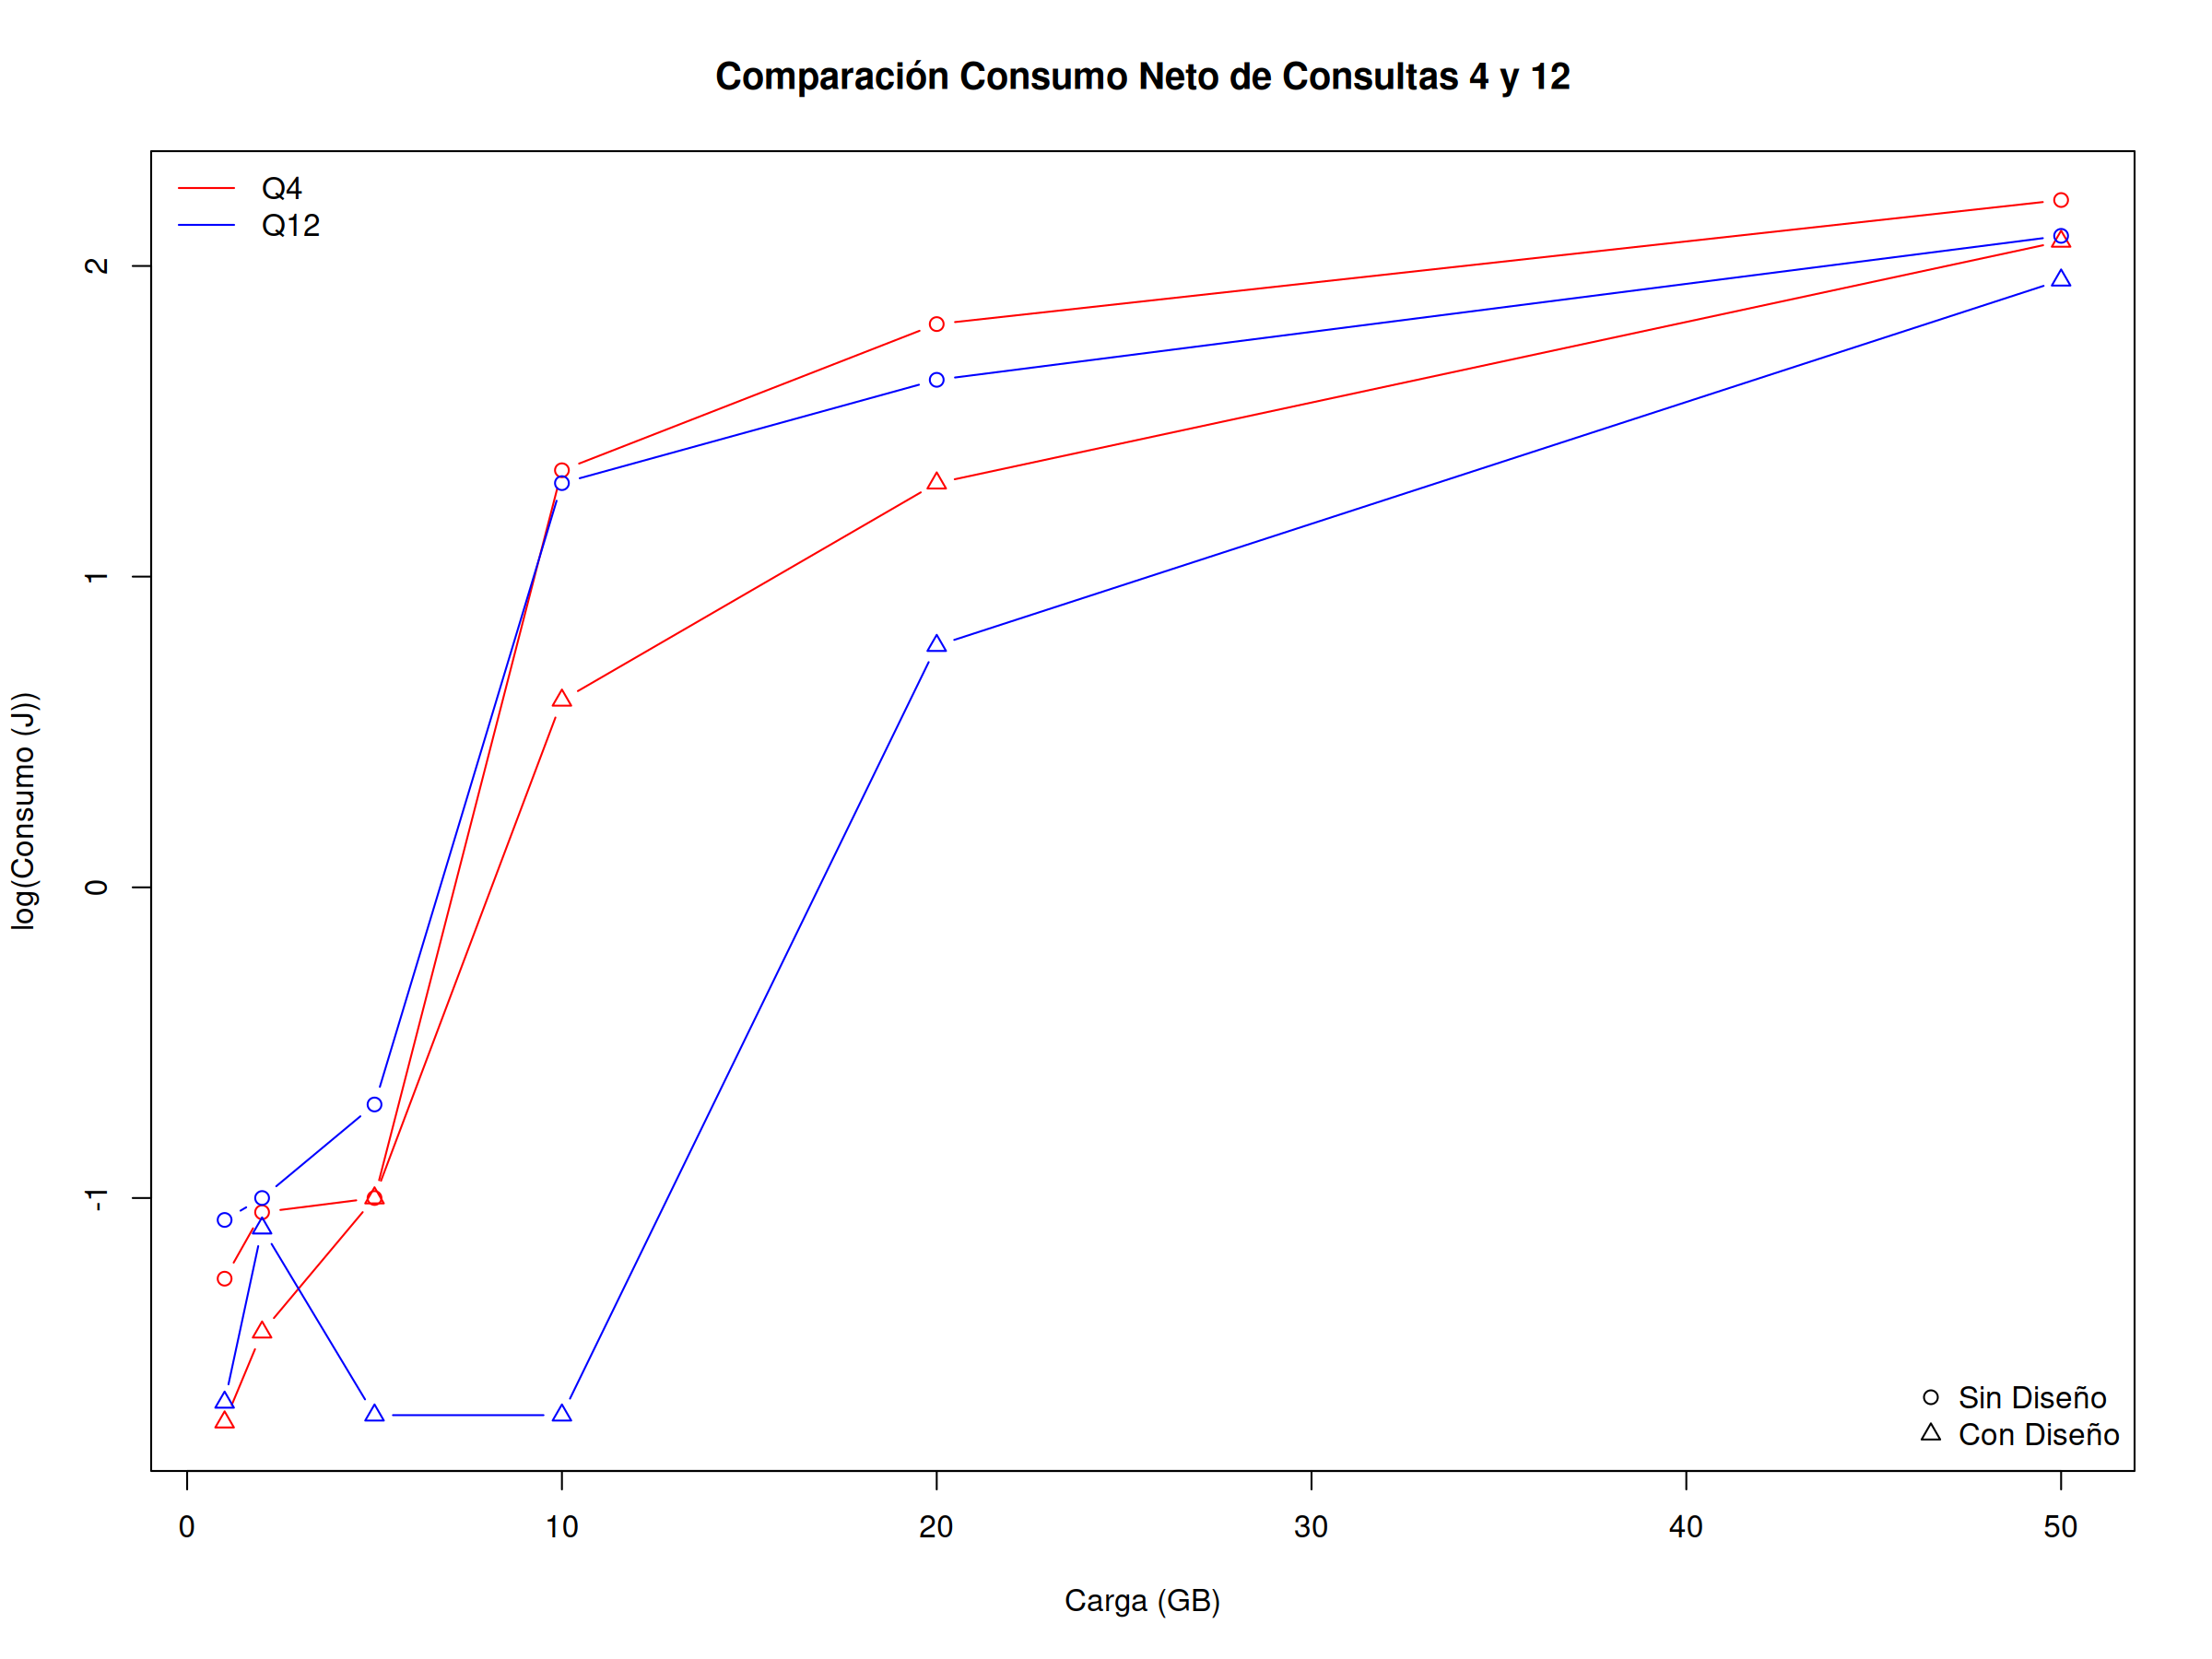
\includegraphics[width = 0.49\textwidth]{images/defensa/cBajo1.png}
          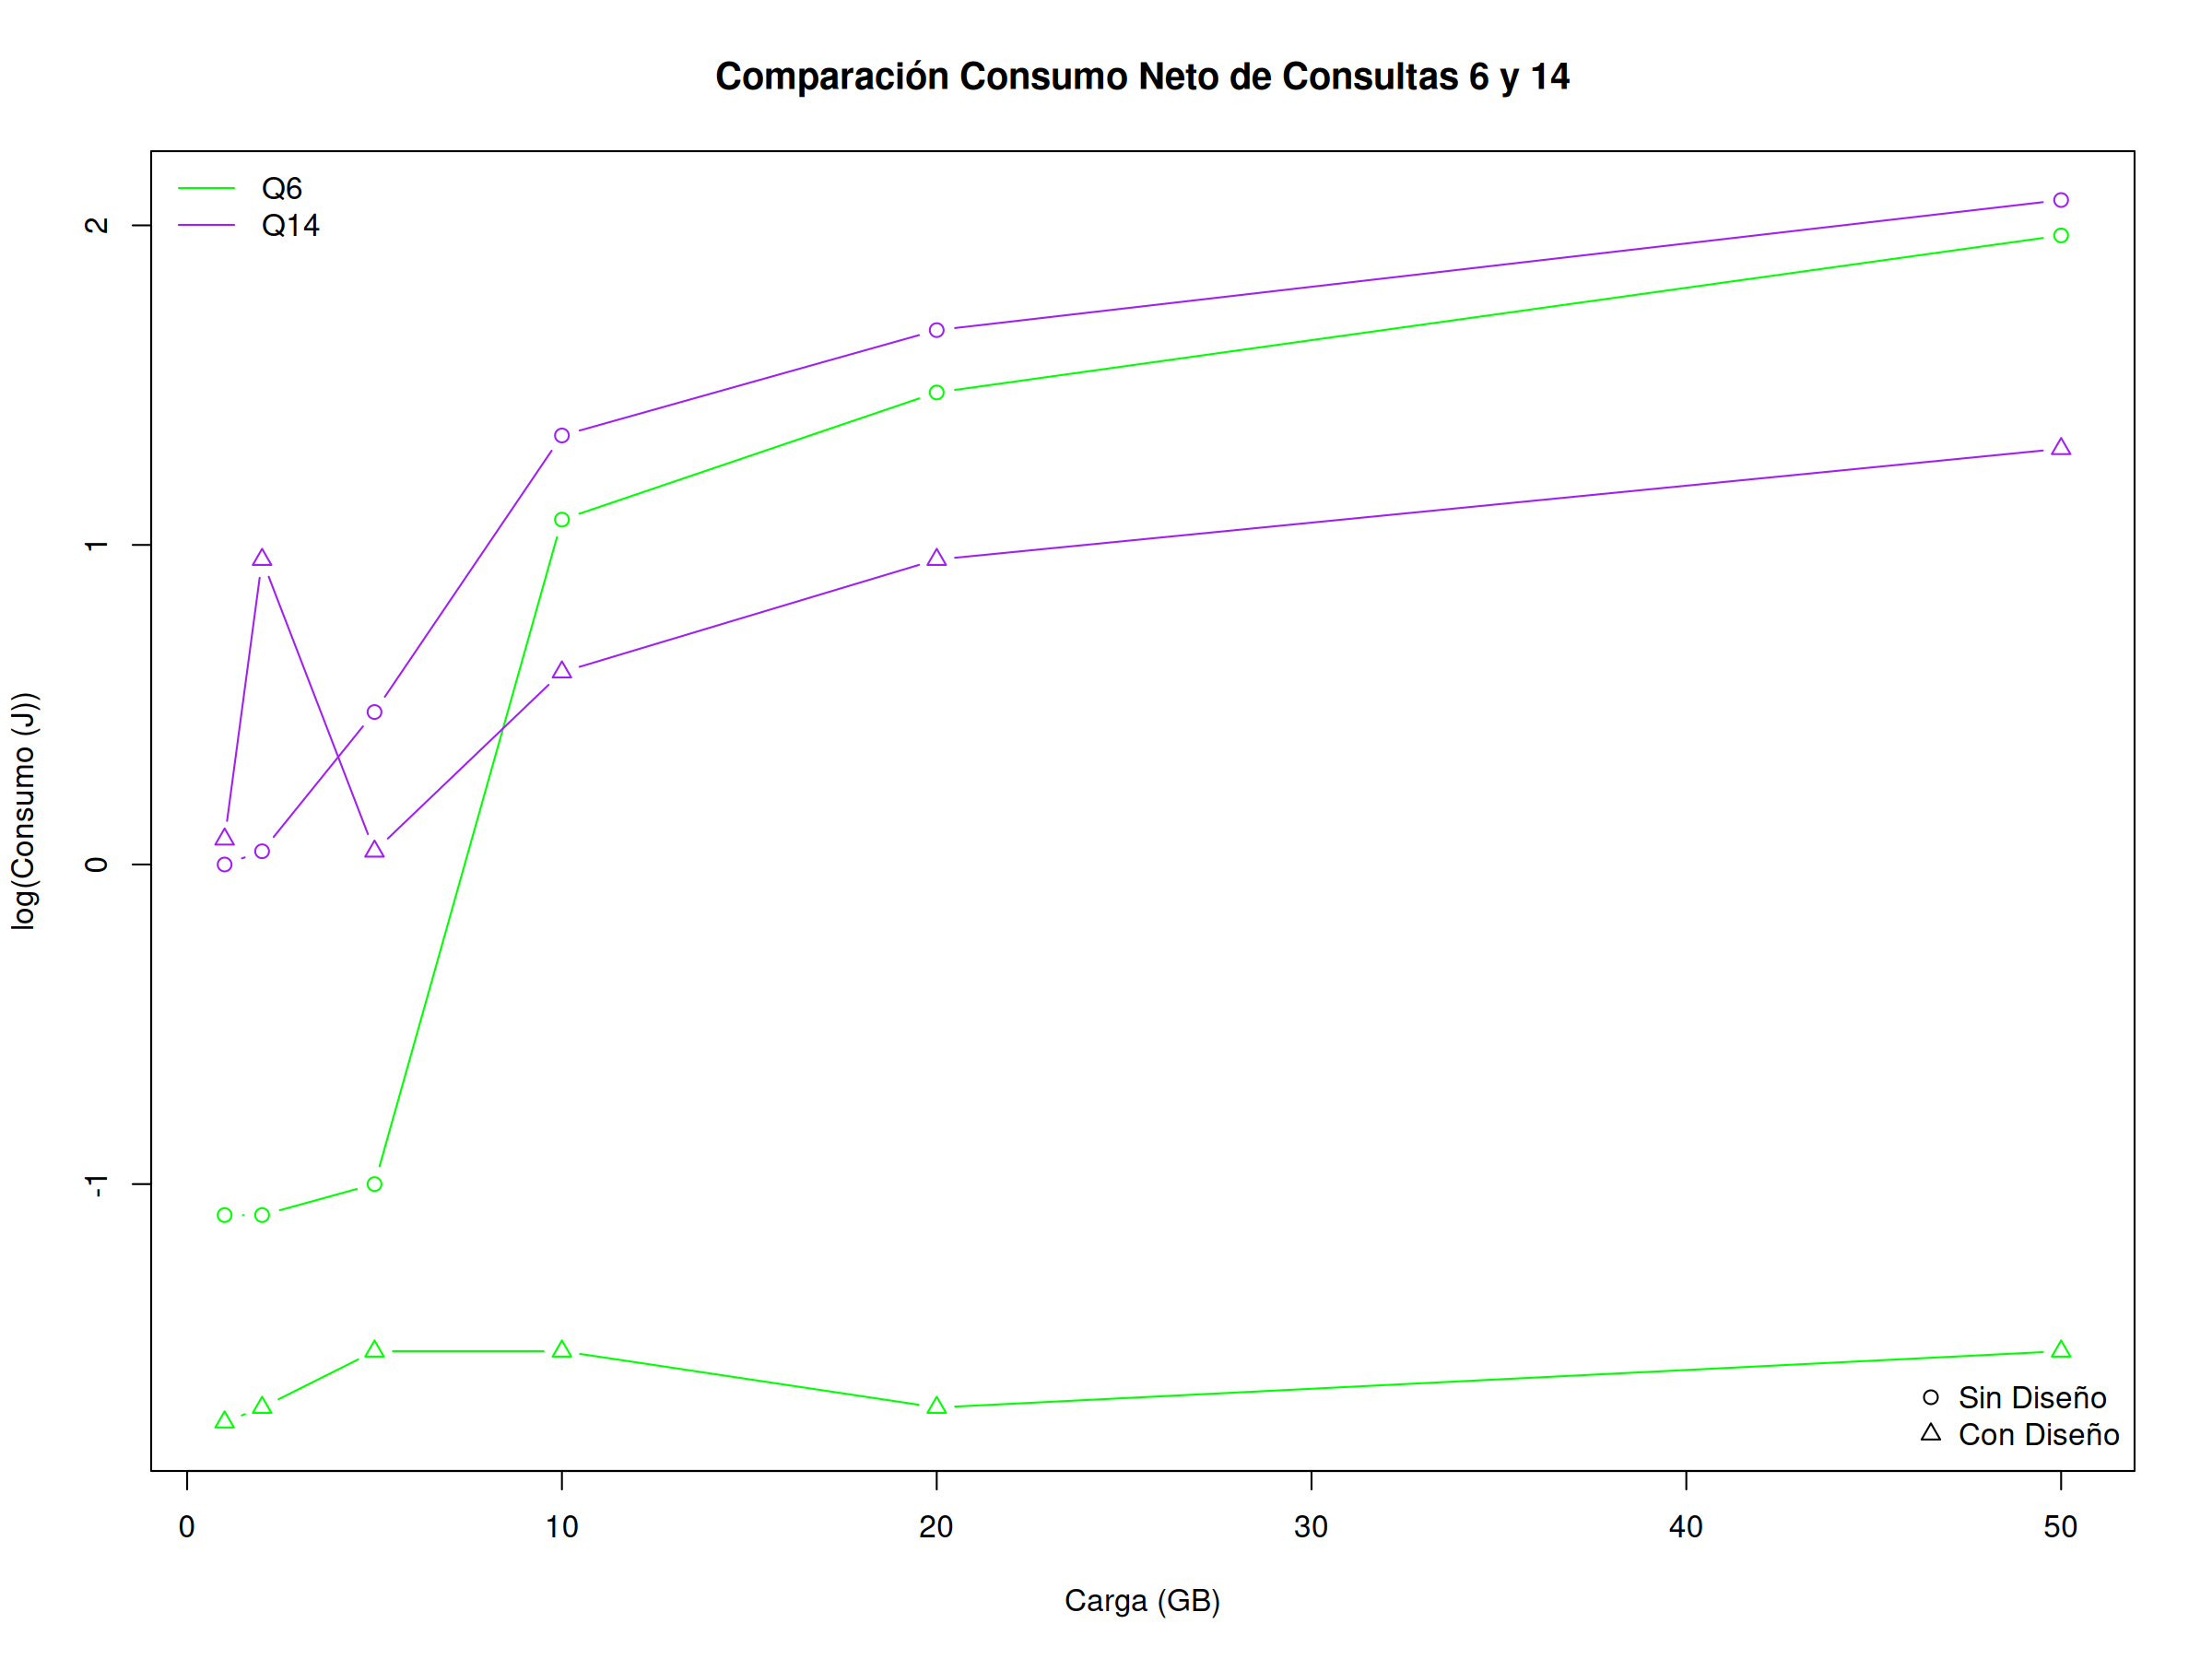
\includegraphics[width = 0.49\textwidth]{images/defensa/cBajo2.png}
          \caption{Comparación de consultas: consumo neto (bajo)}
        \end{figure}
      \end{frame}

      \begin{frame}{Consumo medio}
        \begin{figure}
          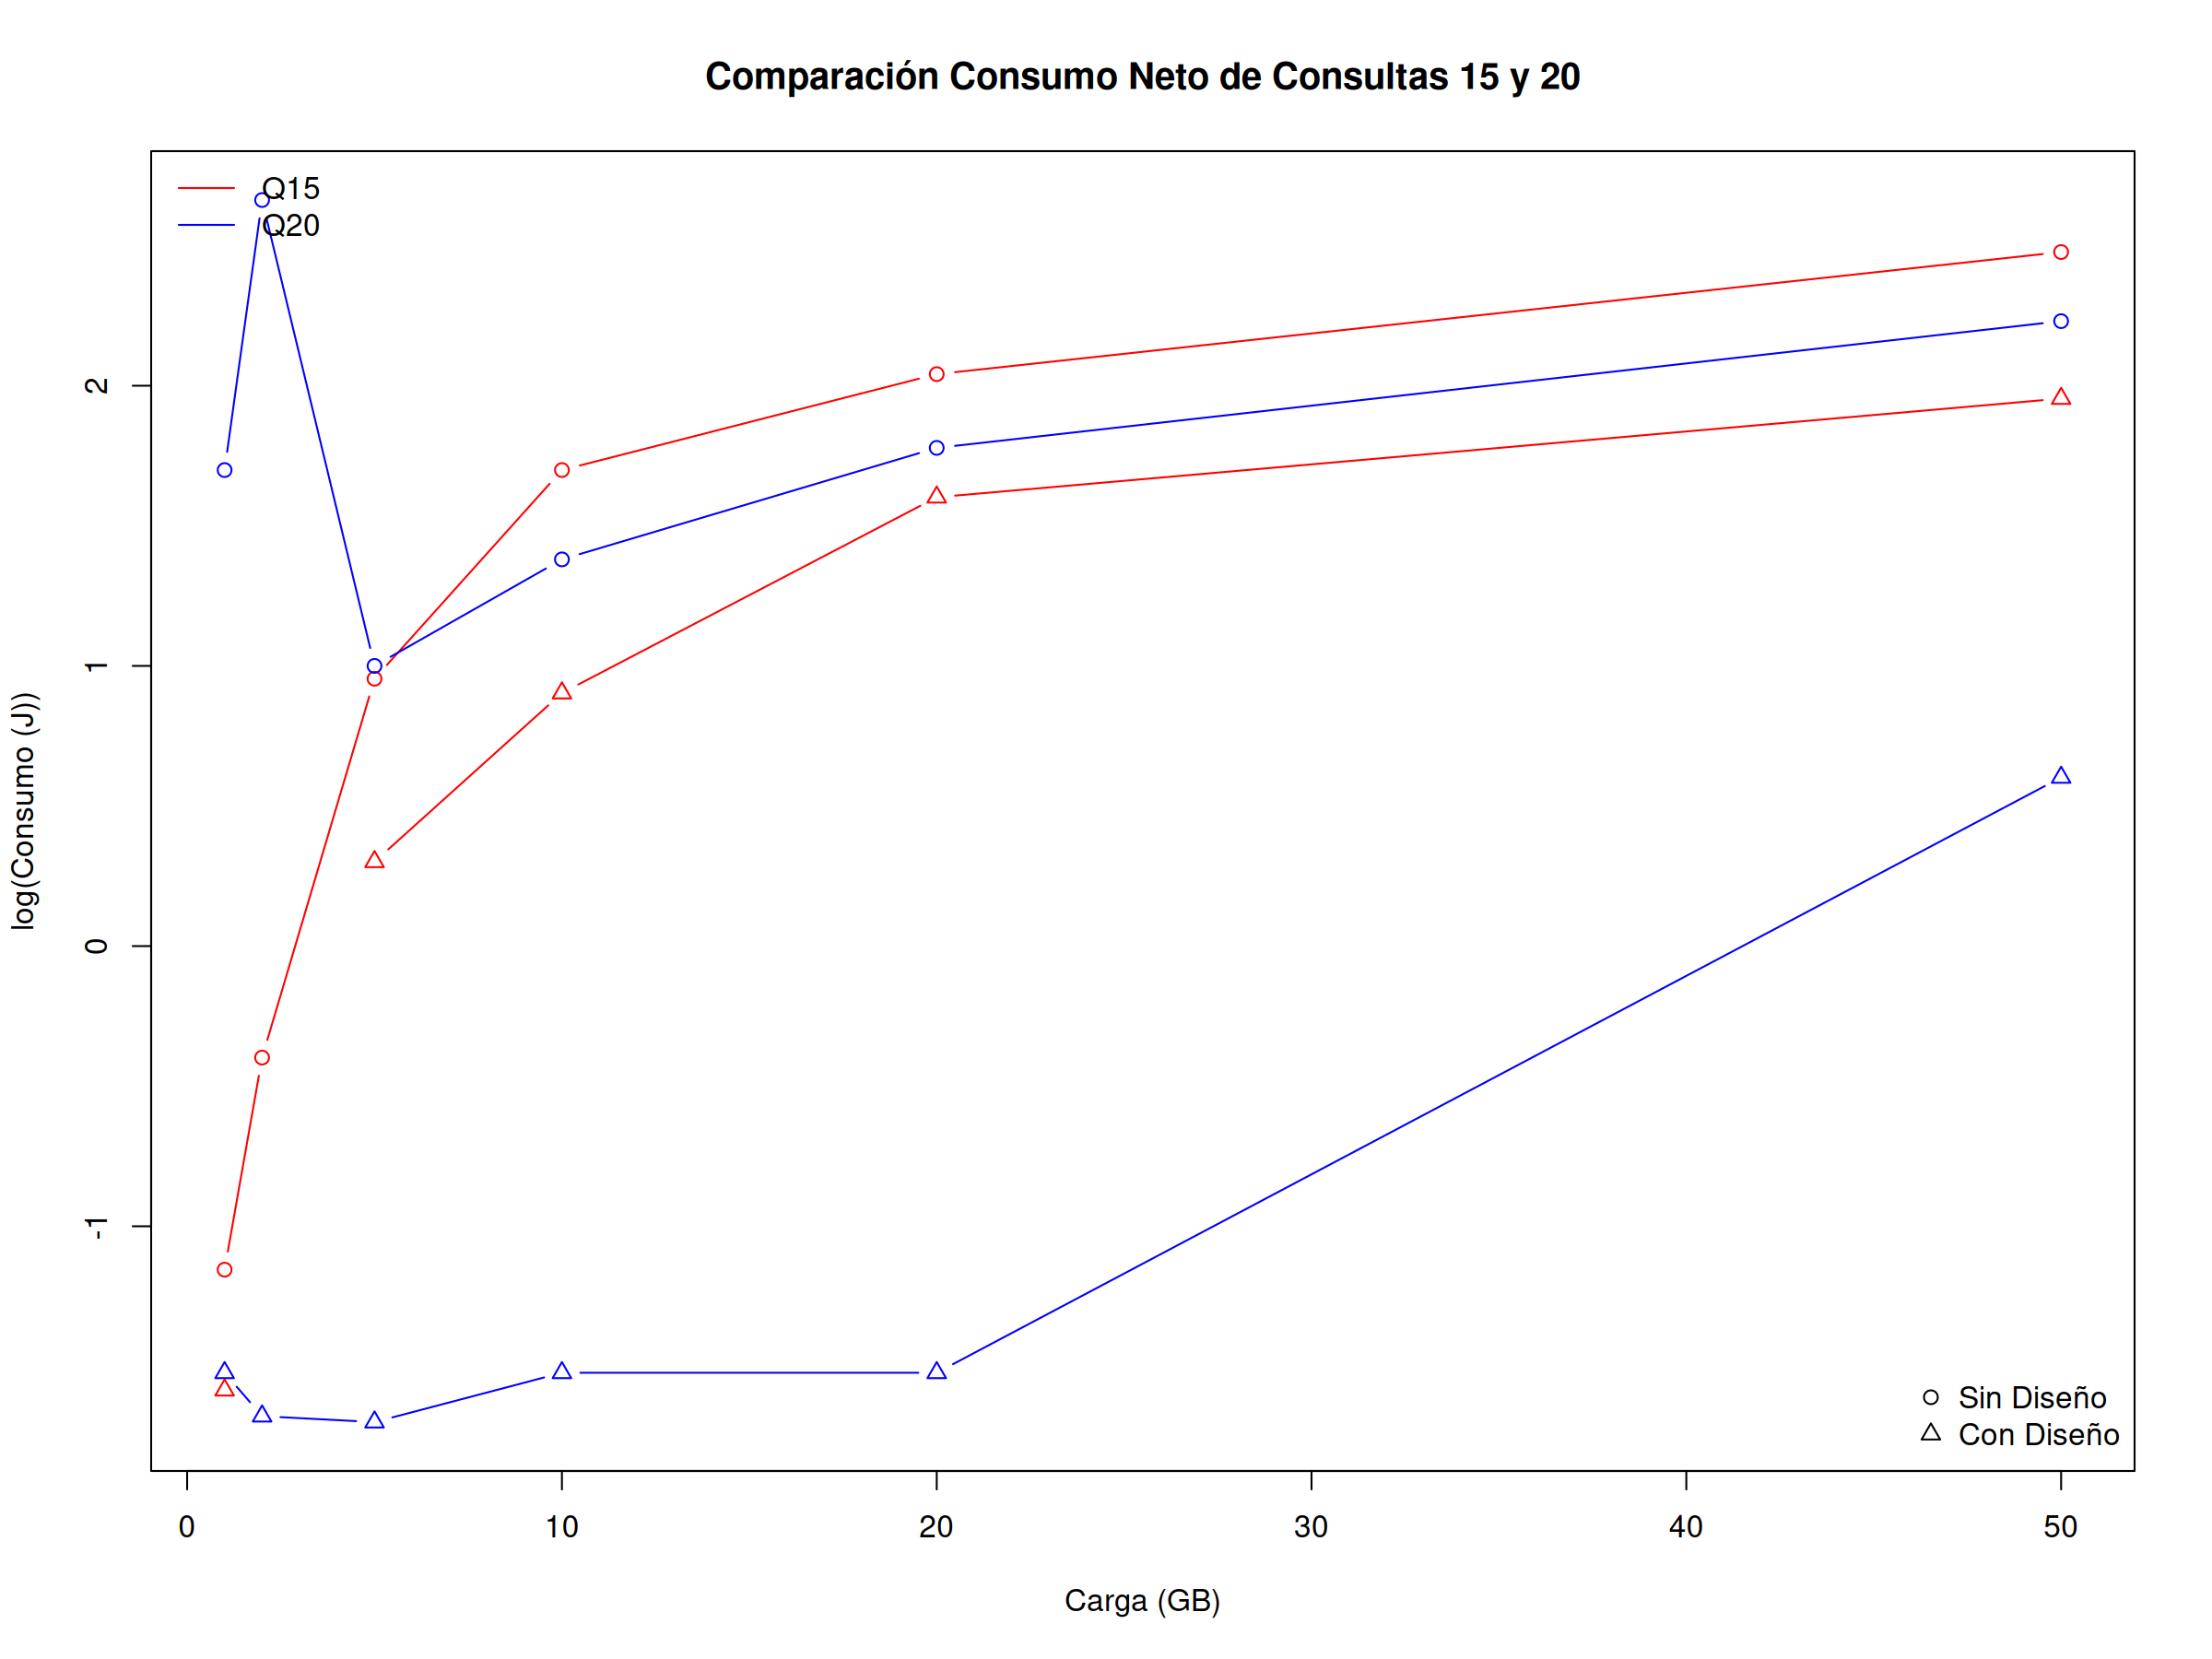
\includegraphics[width = 0.49\textwidth]{images/defensa/cMedio1.png}
          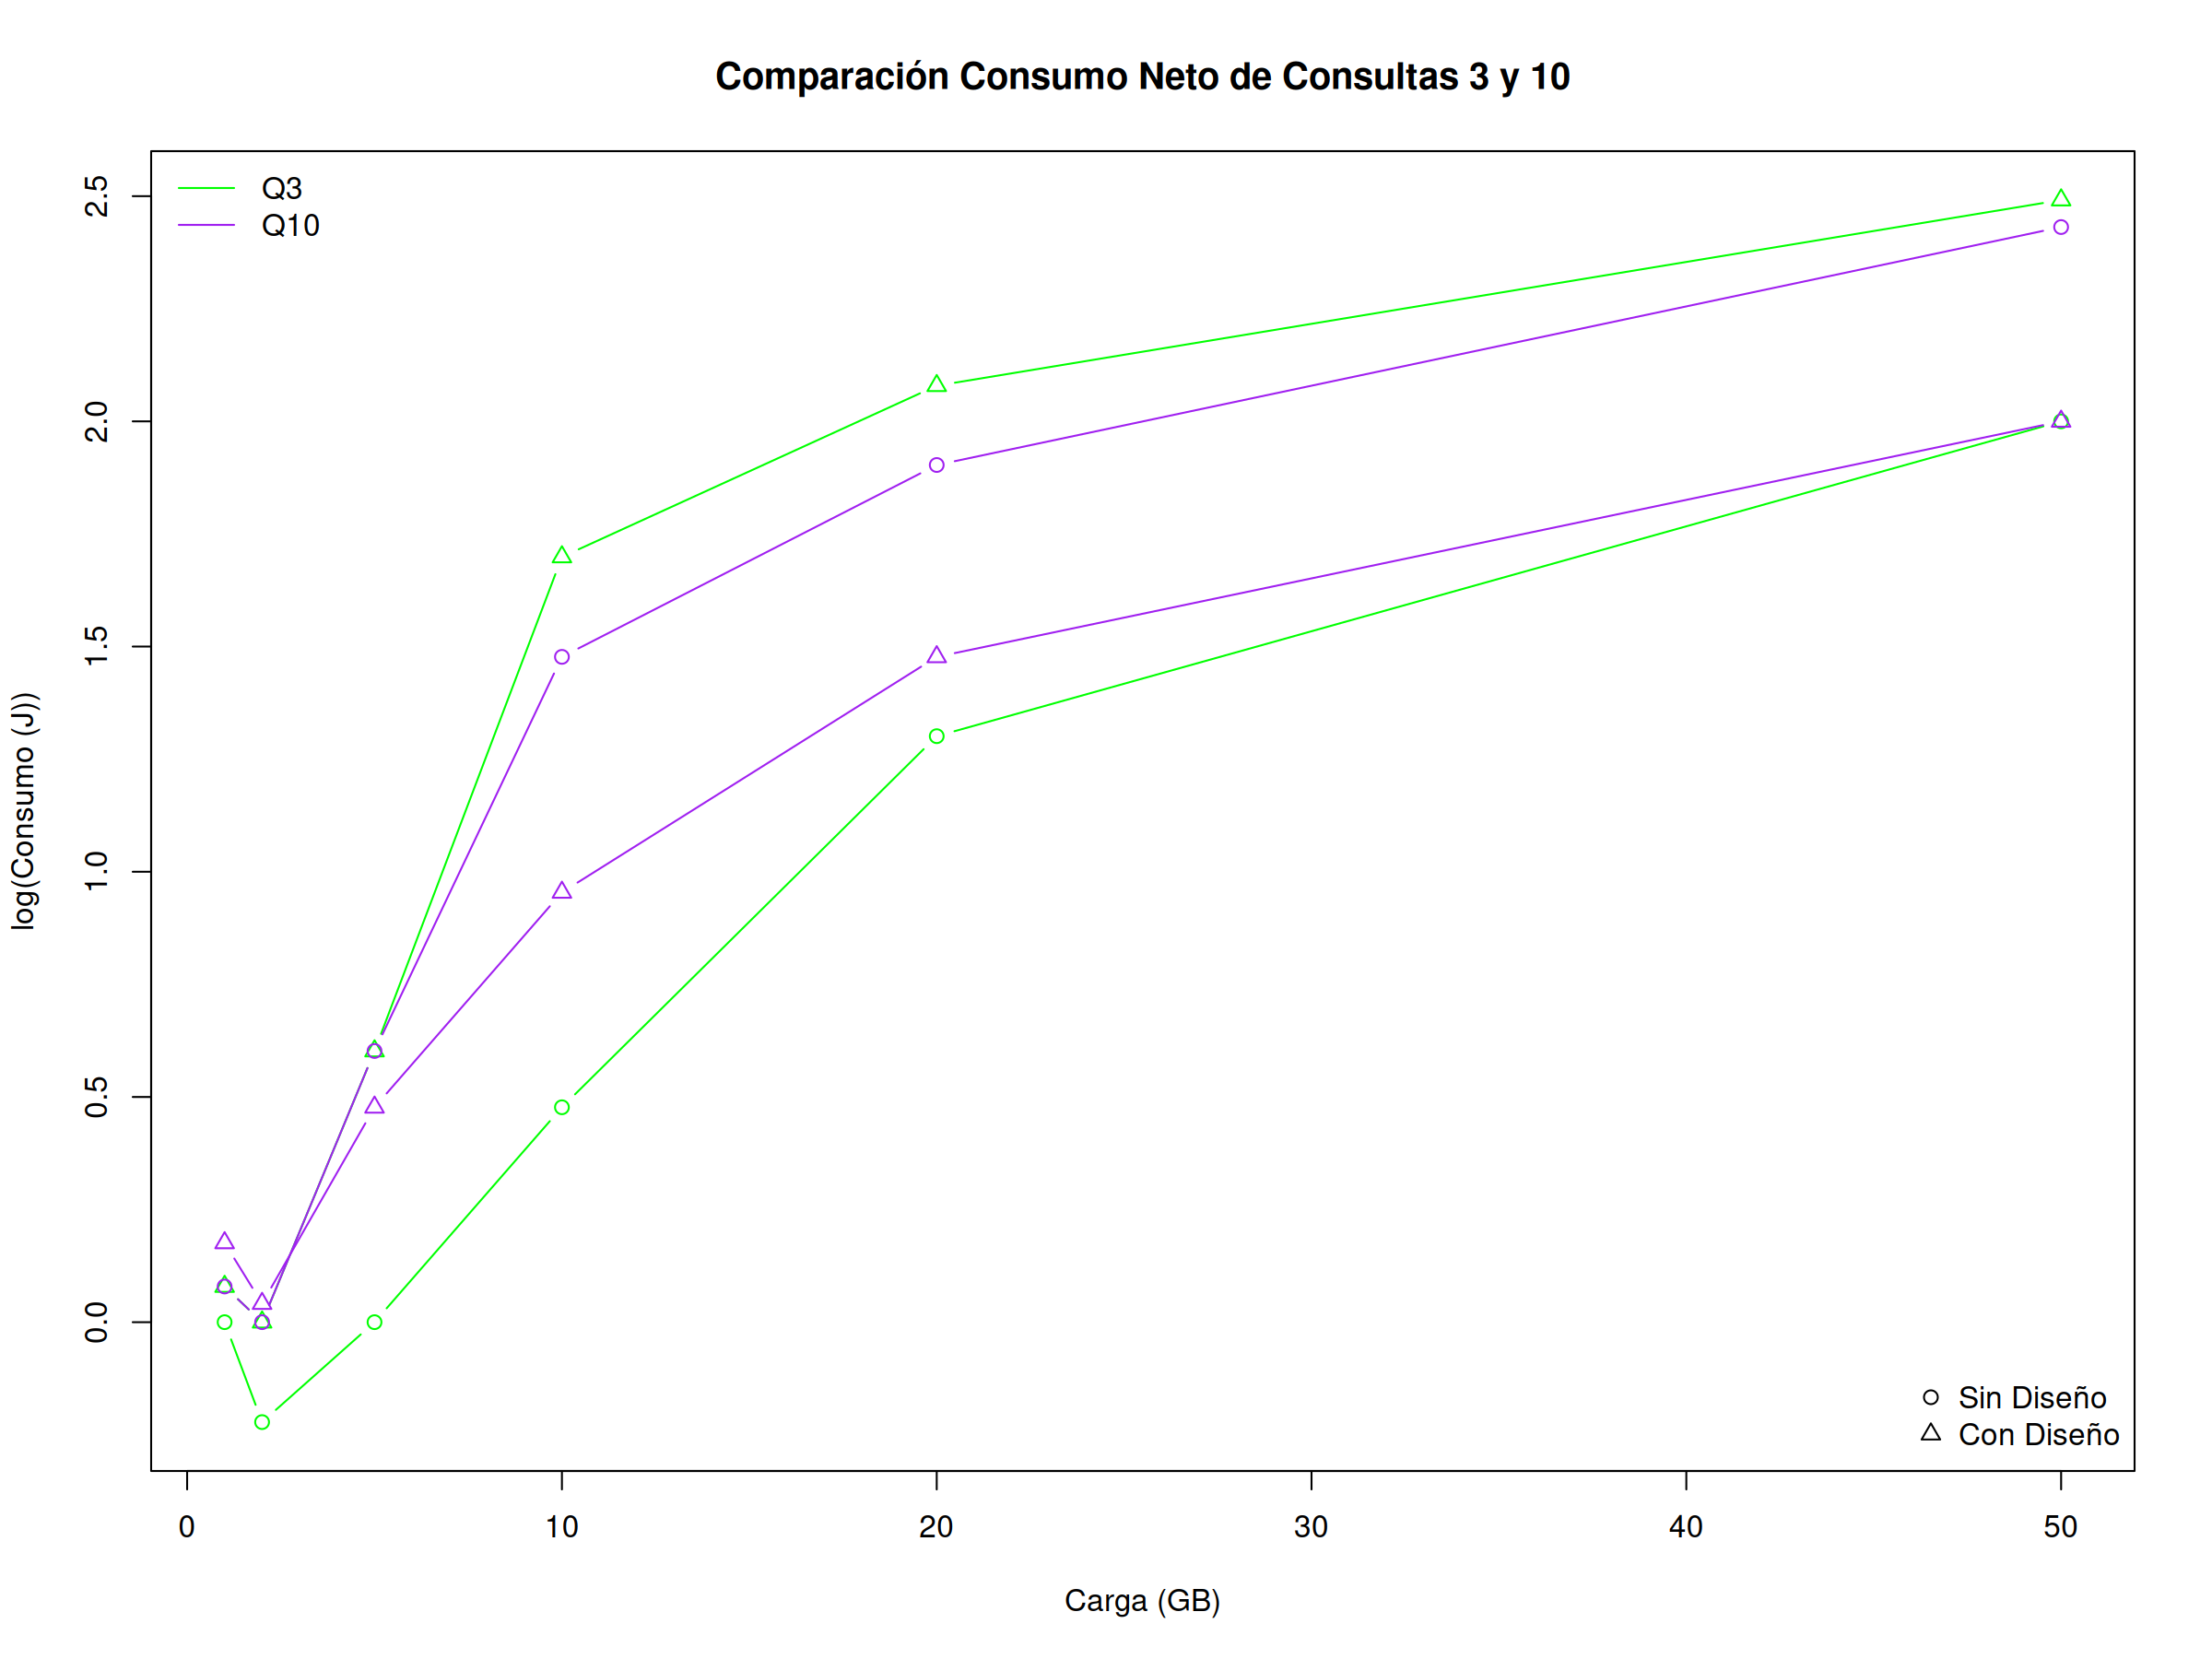
\includegraphics[width = 0.49\textwidth]{images/defensa/cMedio2.png}
          \caption{Comparación de consultas: consumo neto (medio)}
        \end{figure}
      \end{frame}

      \begin{frame}{Consumo medio}
        \begin{figure}
          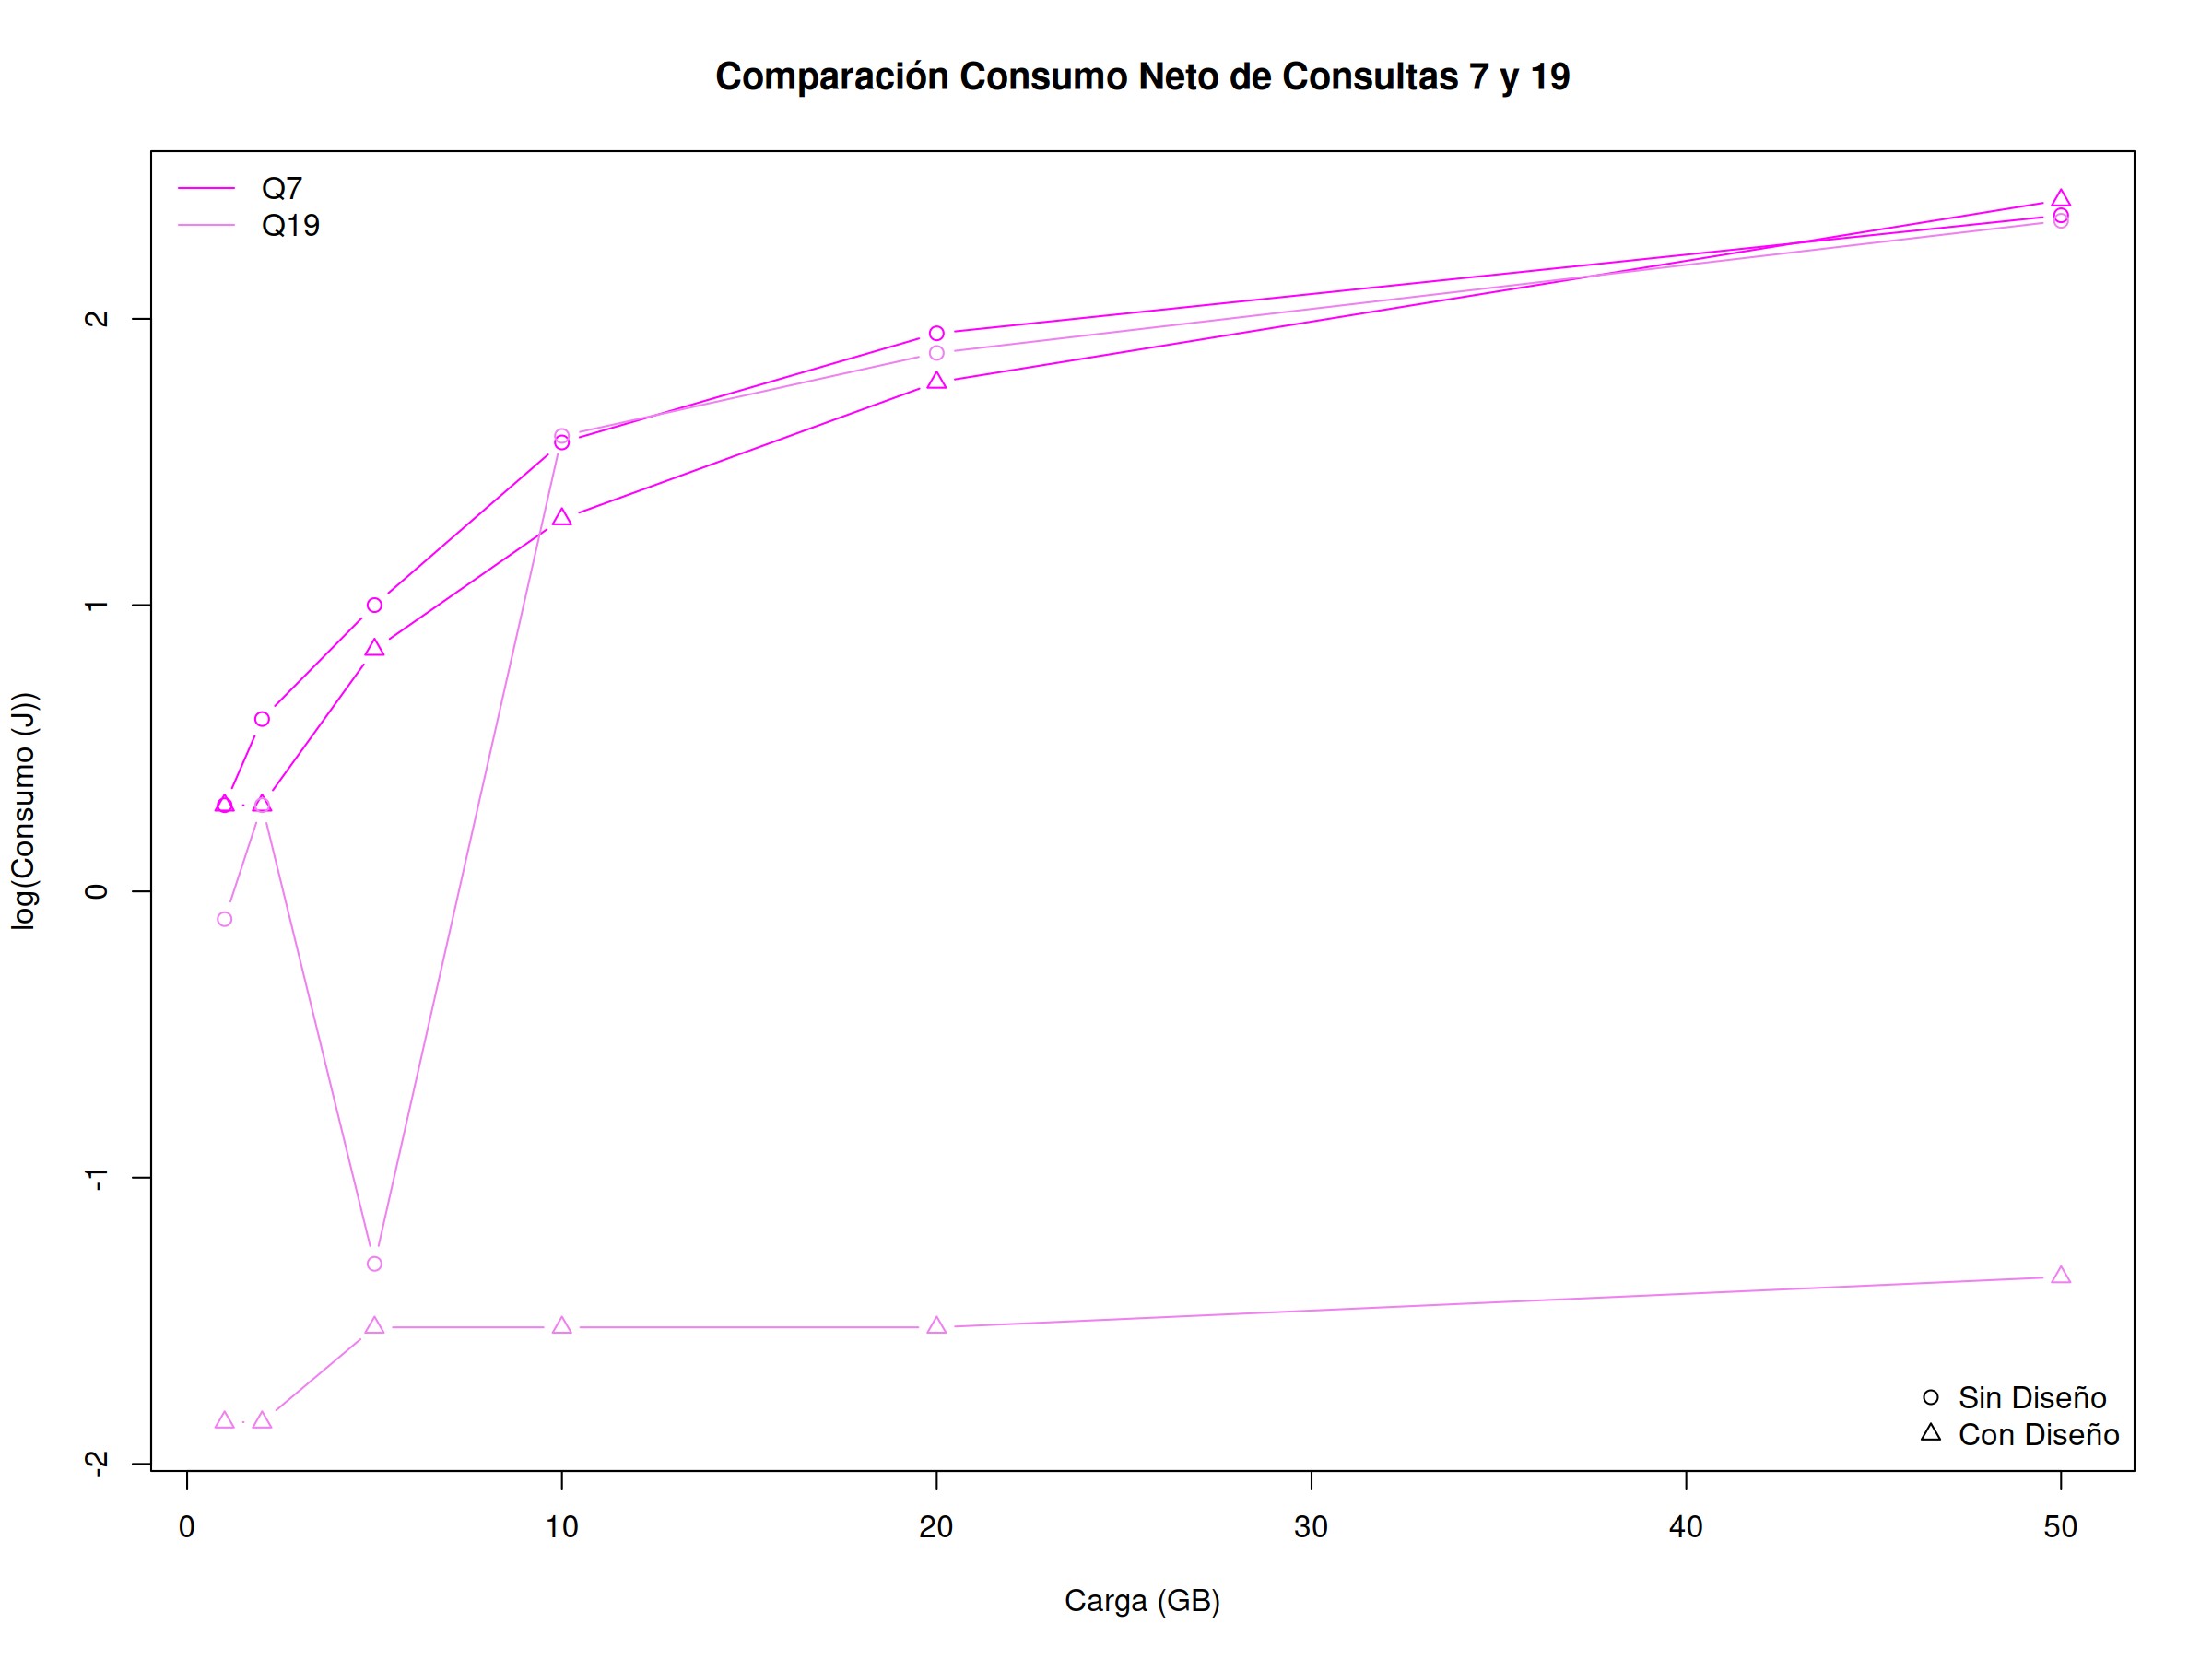
\includegraphics[width = 0.75\textwidth]{images/defensa/cMedio3.png}
          \caption{Comparación de consultas: consumo neto (medio)}
        \end{figure}
      \end{frame}

      \begin{frame}{Consumo alto}
        \begin{figure}
          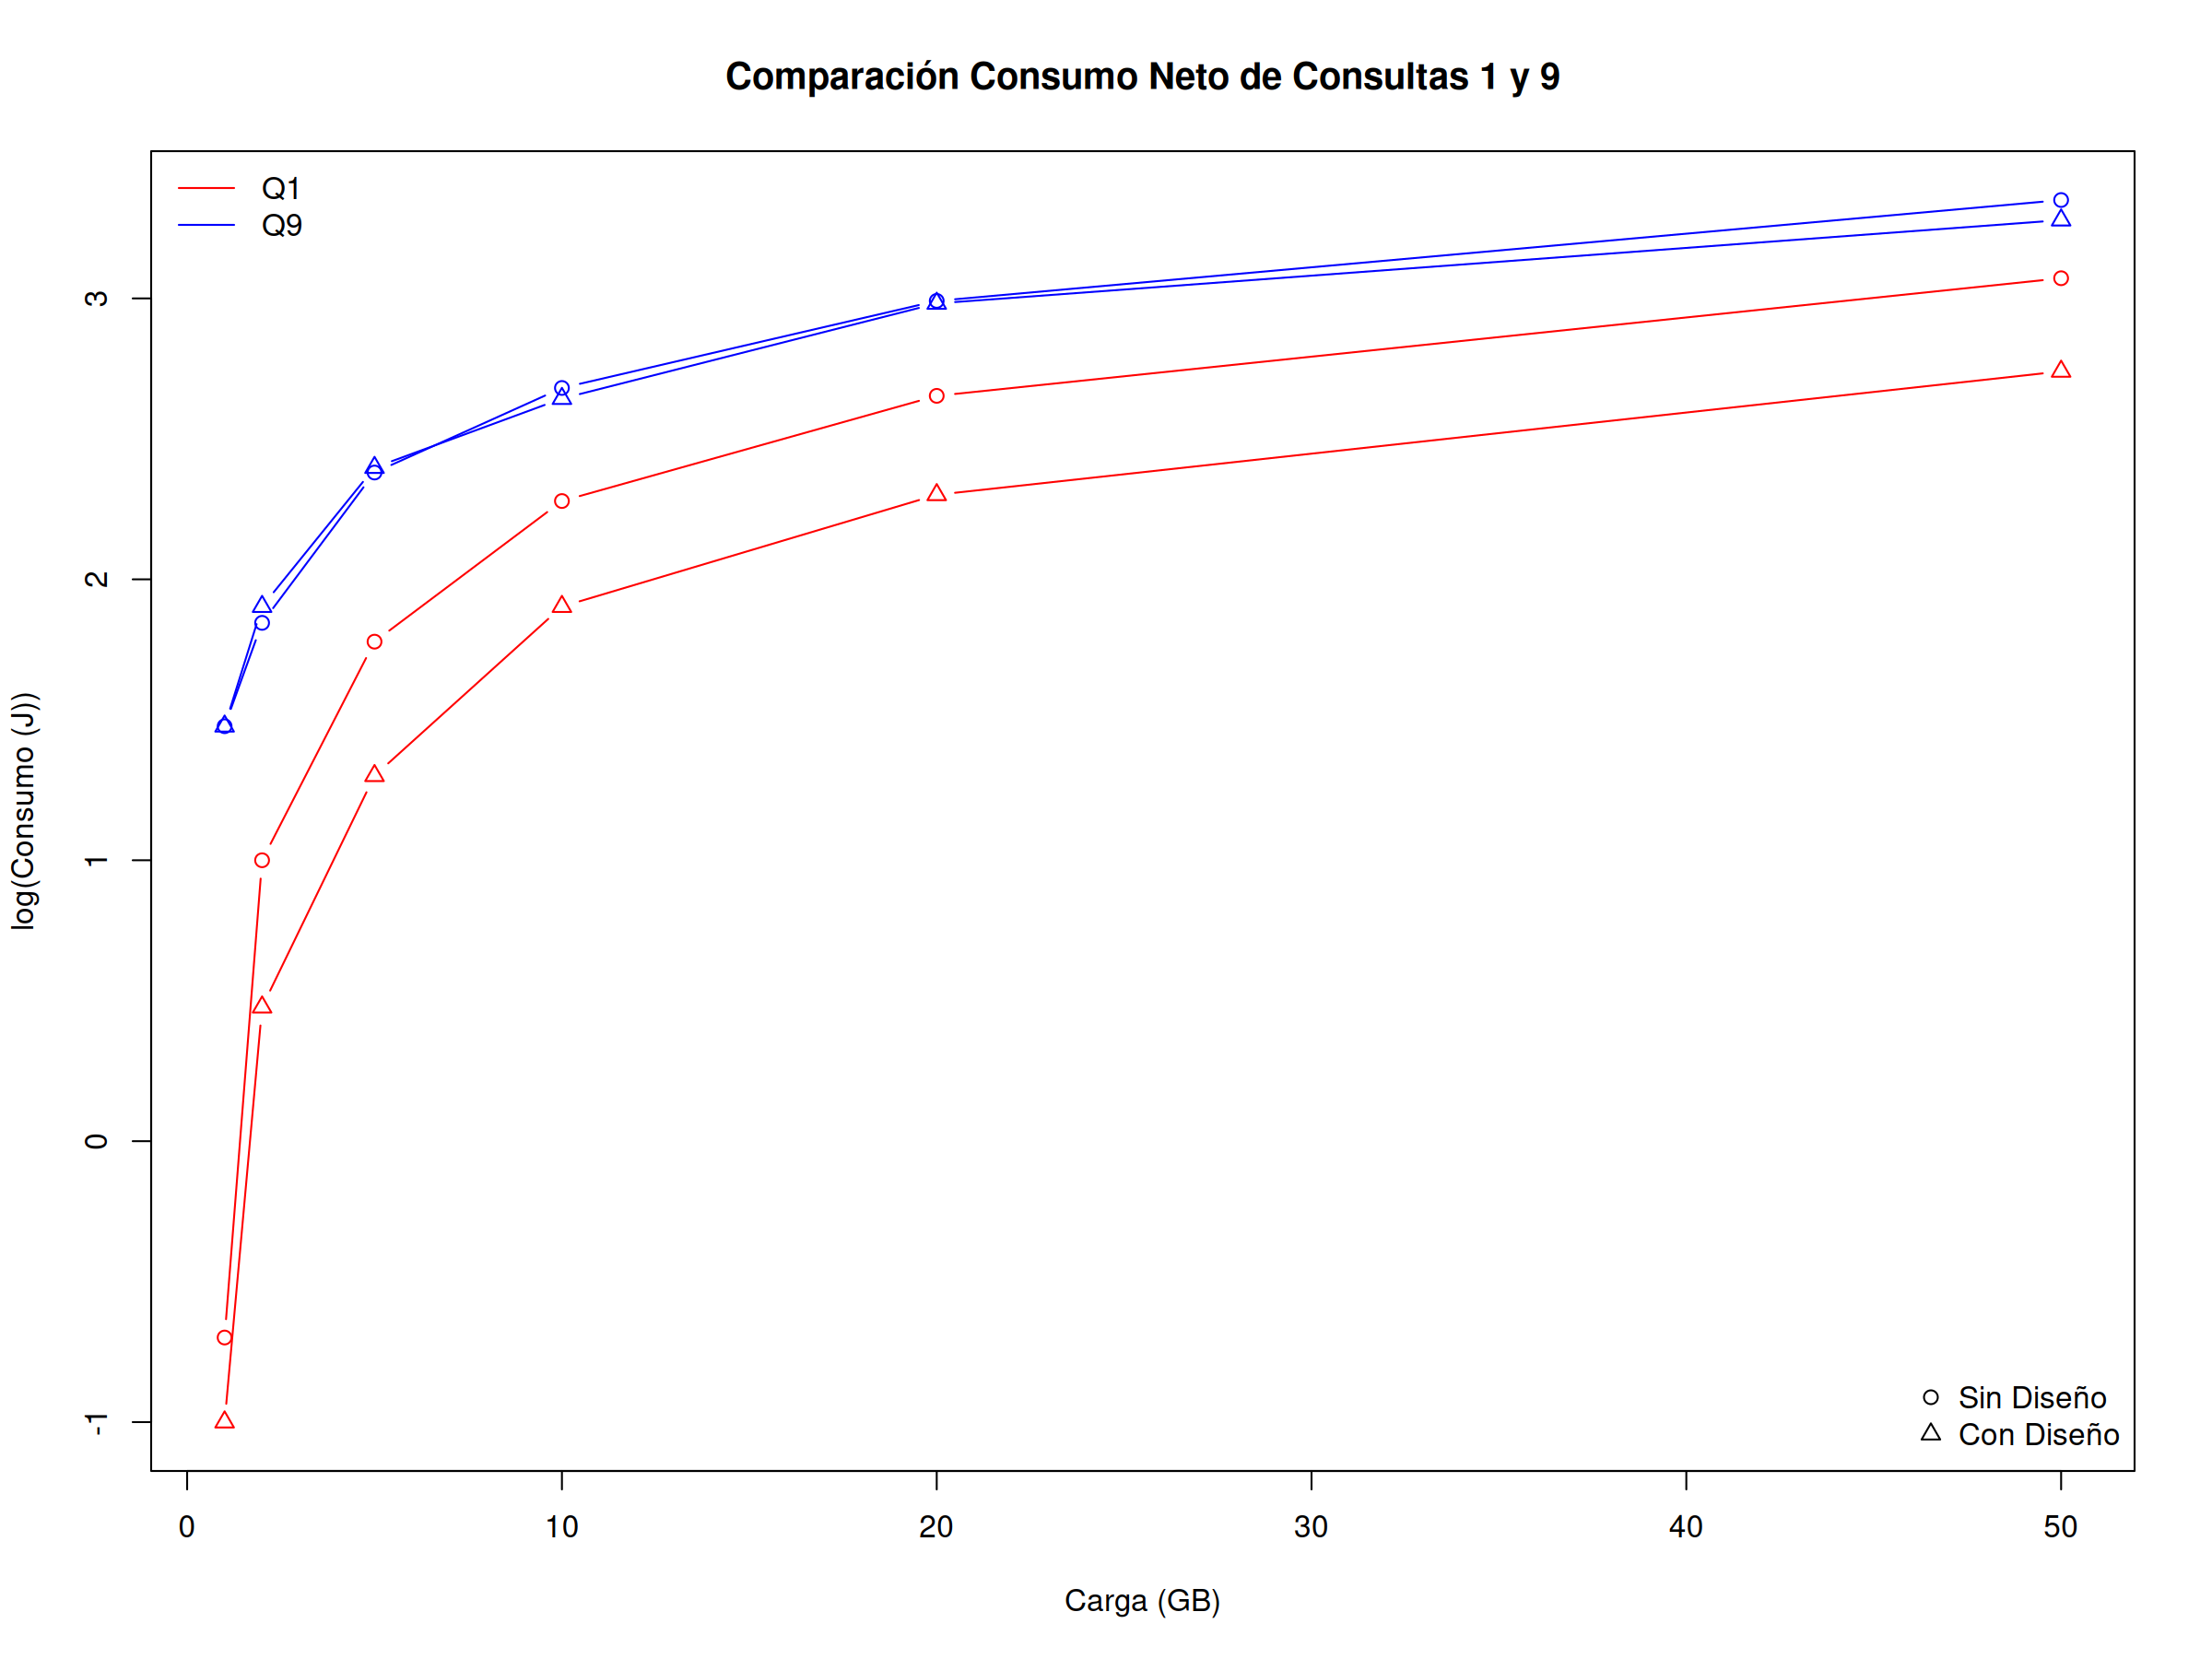
\includegraphics[width = 0.49\textwidth]{images/defensa/cAlto1.png}
          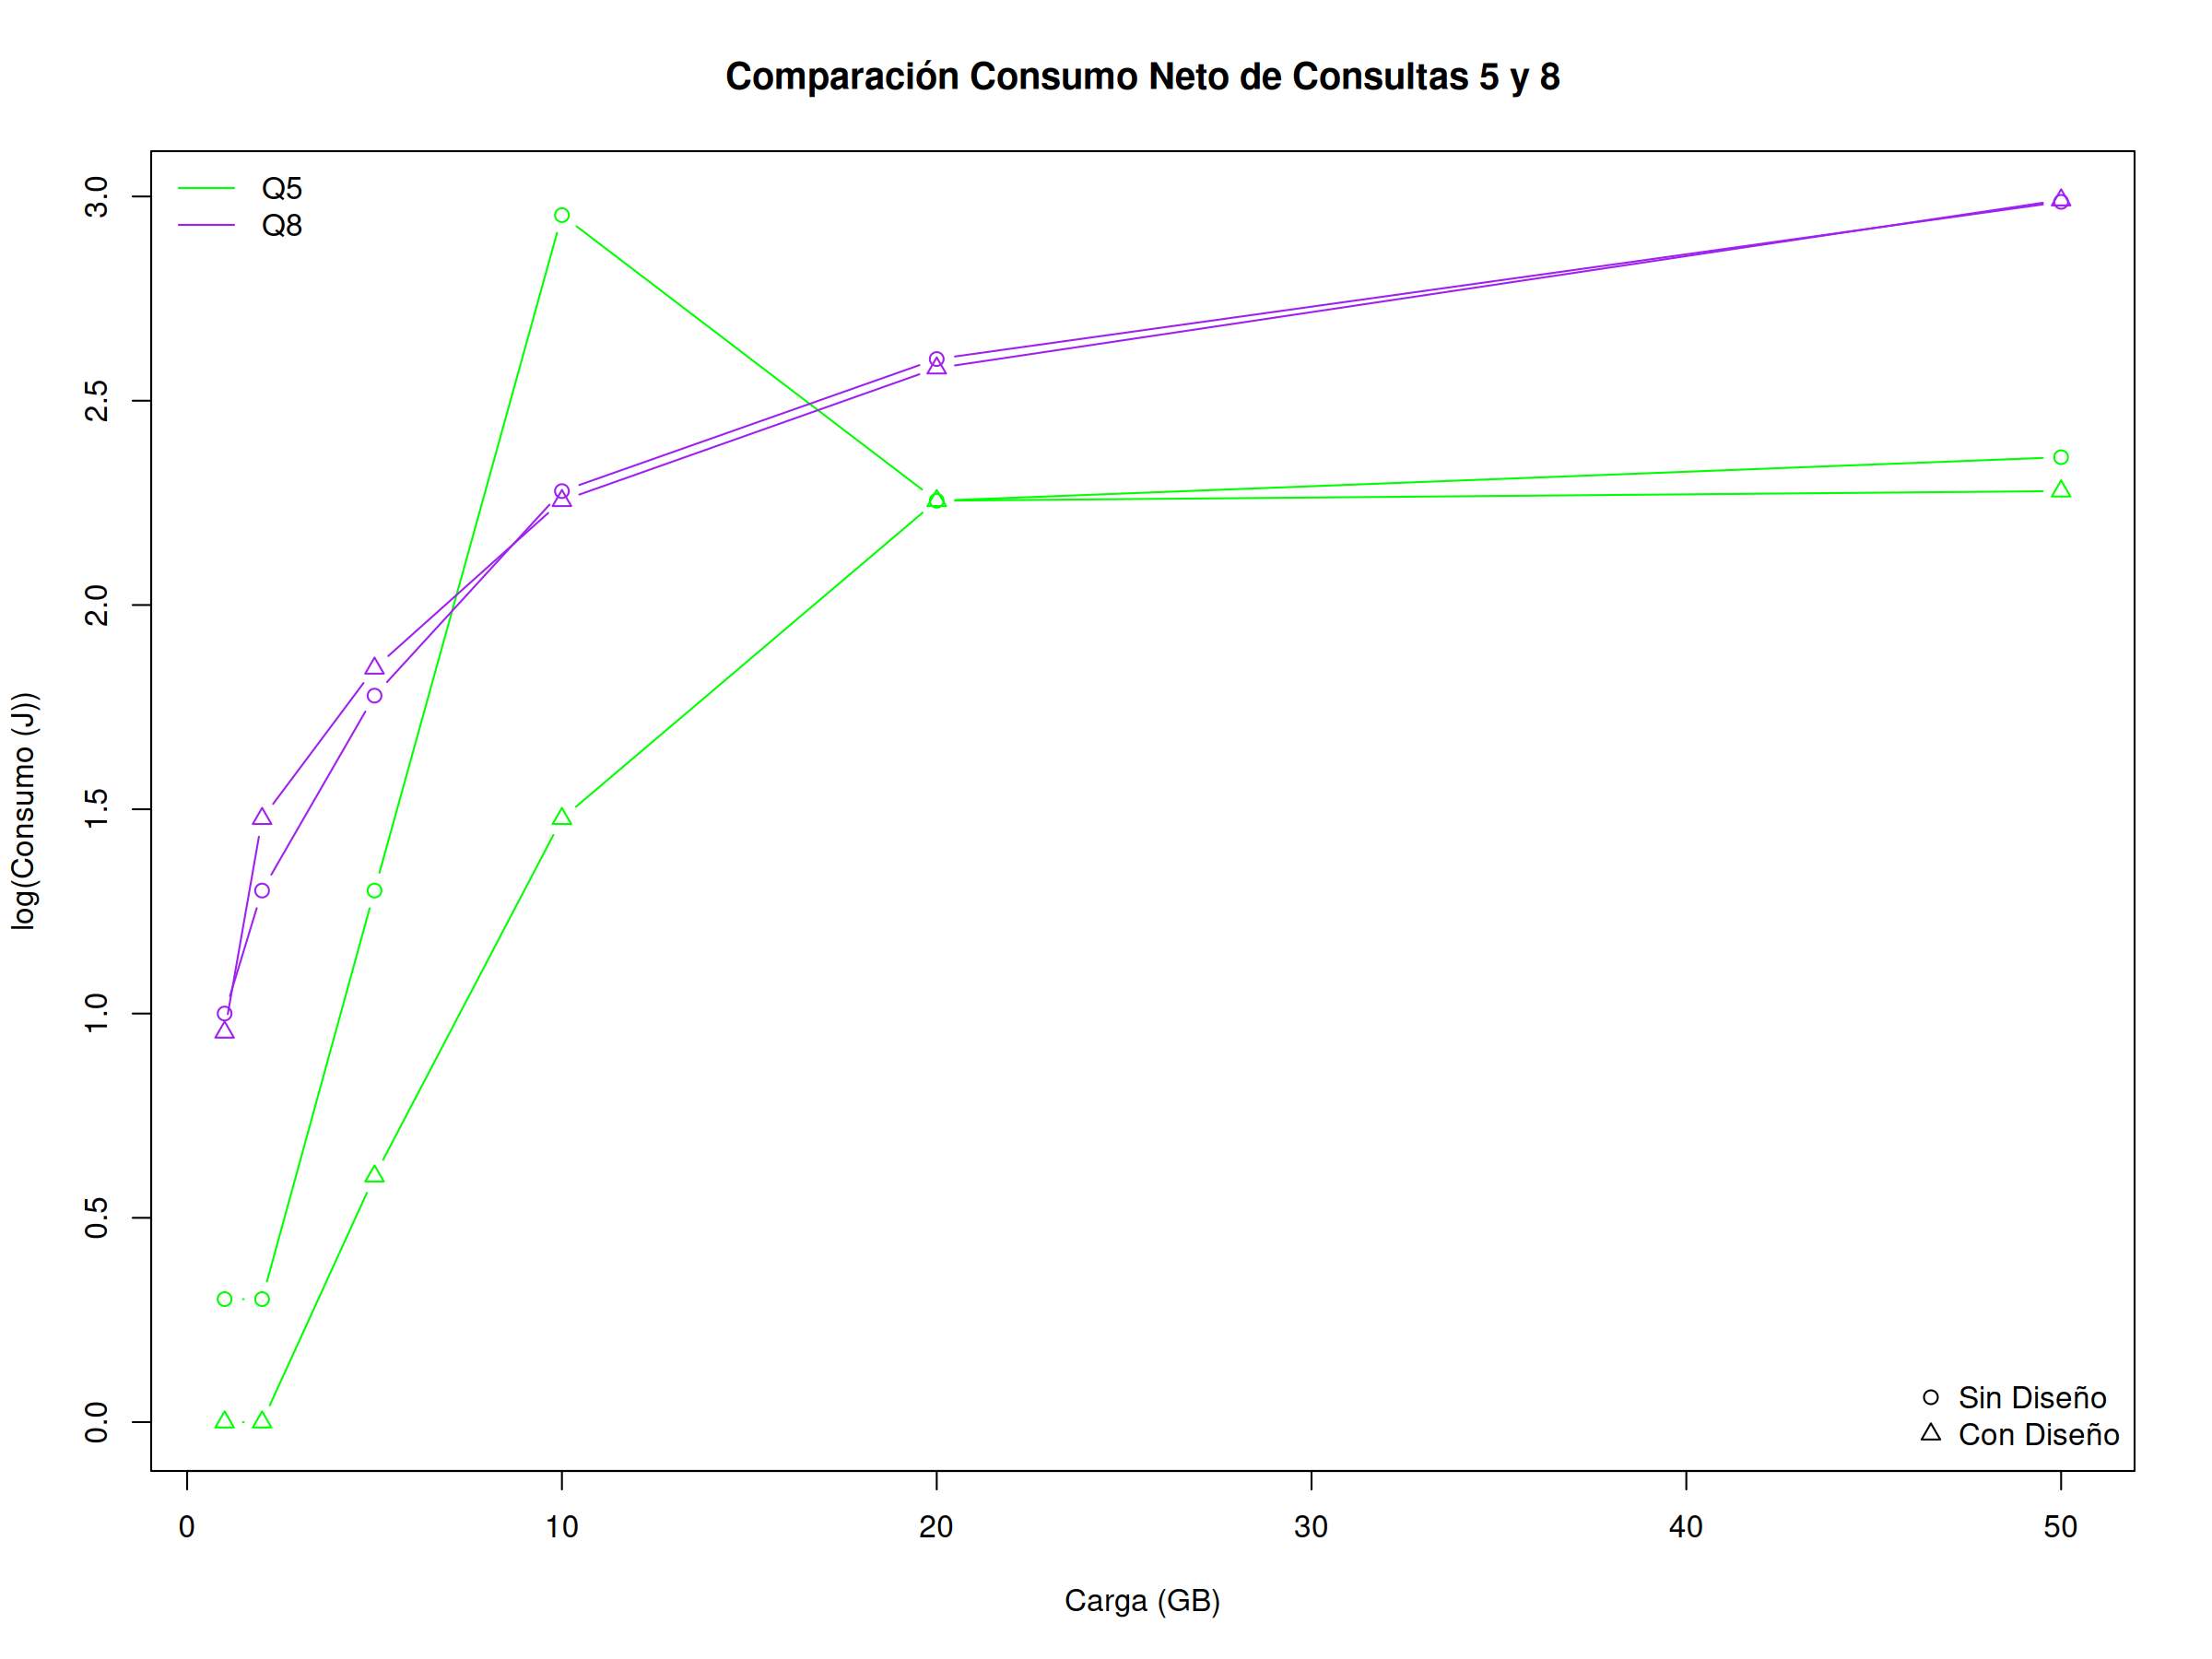
\includegraphics[width = 0.49\textwidth]{images/defensa/cAlto2.png}
          \caption{Comparación de consultas: consumo neto (alto)}
        \end{figure}
      \end{frame}

      \begin{frame}{Consumo extremo}
        \begin{figure}
          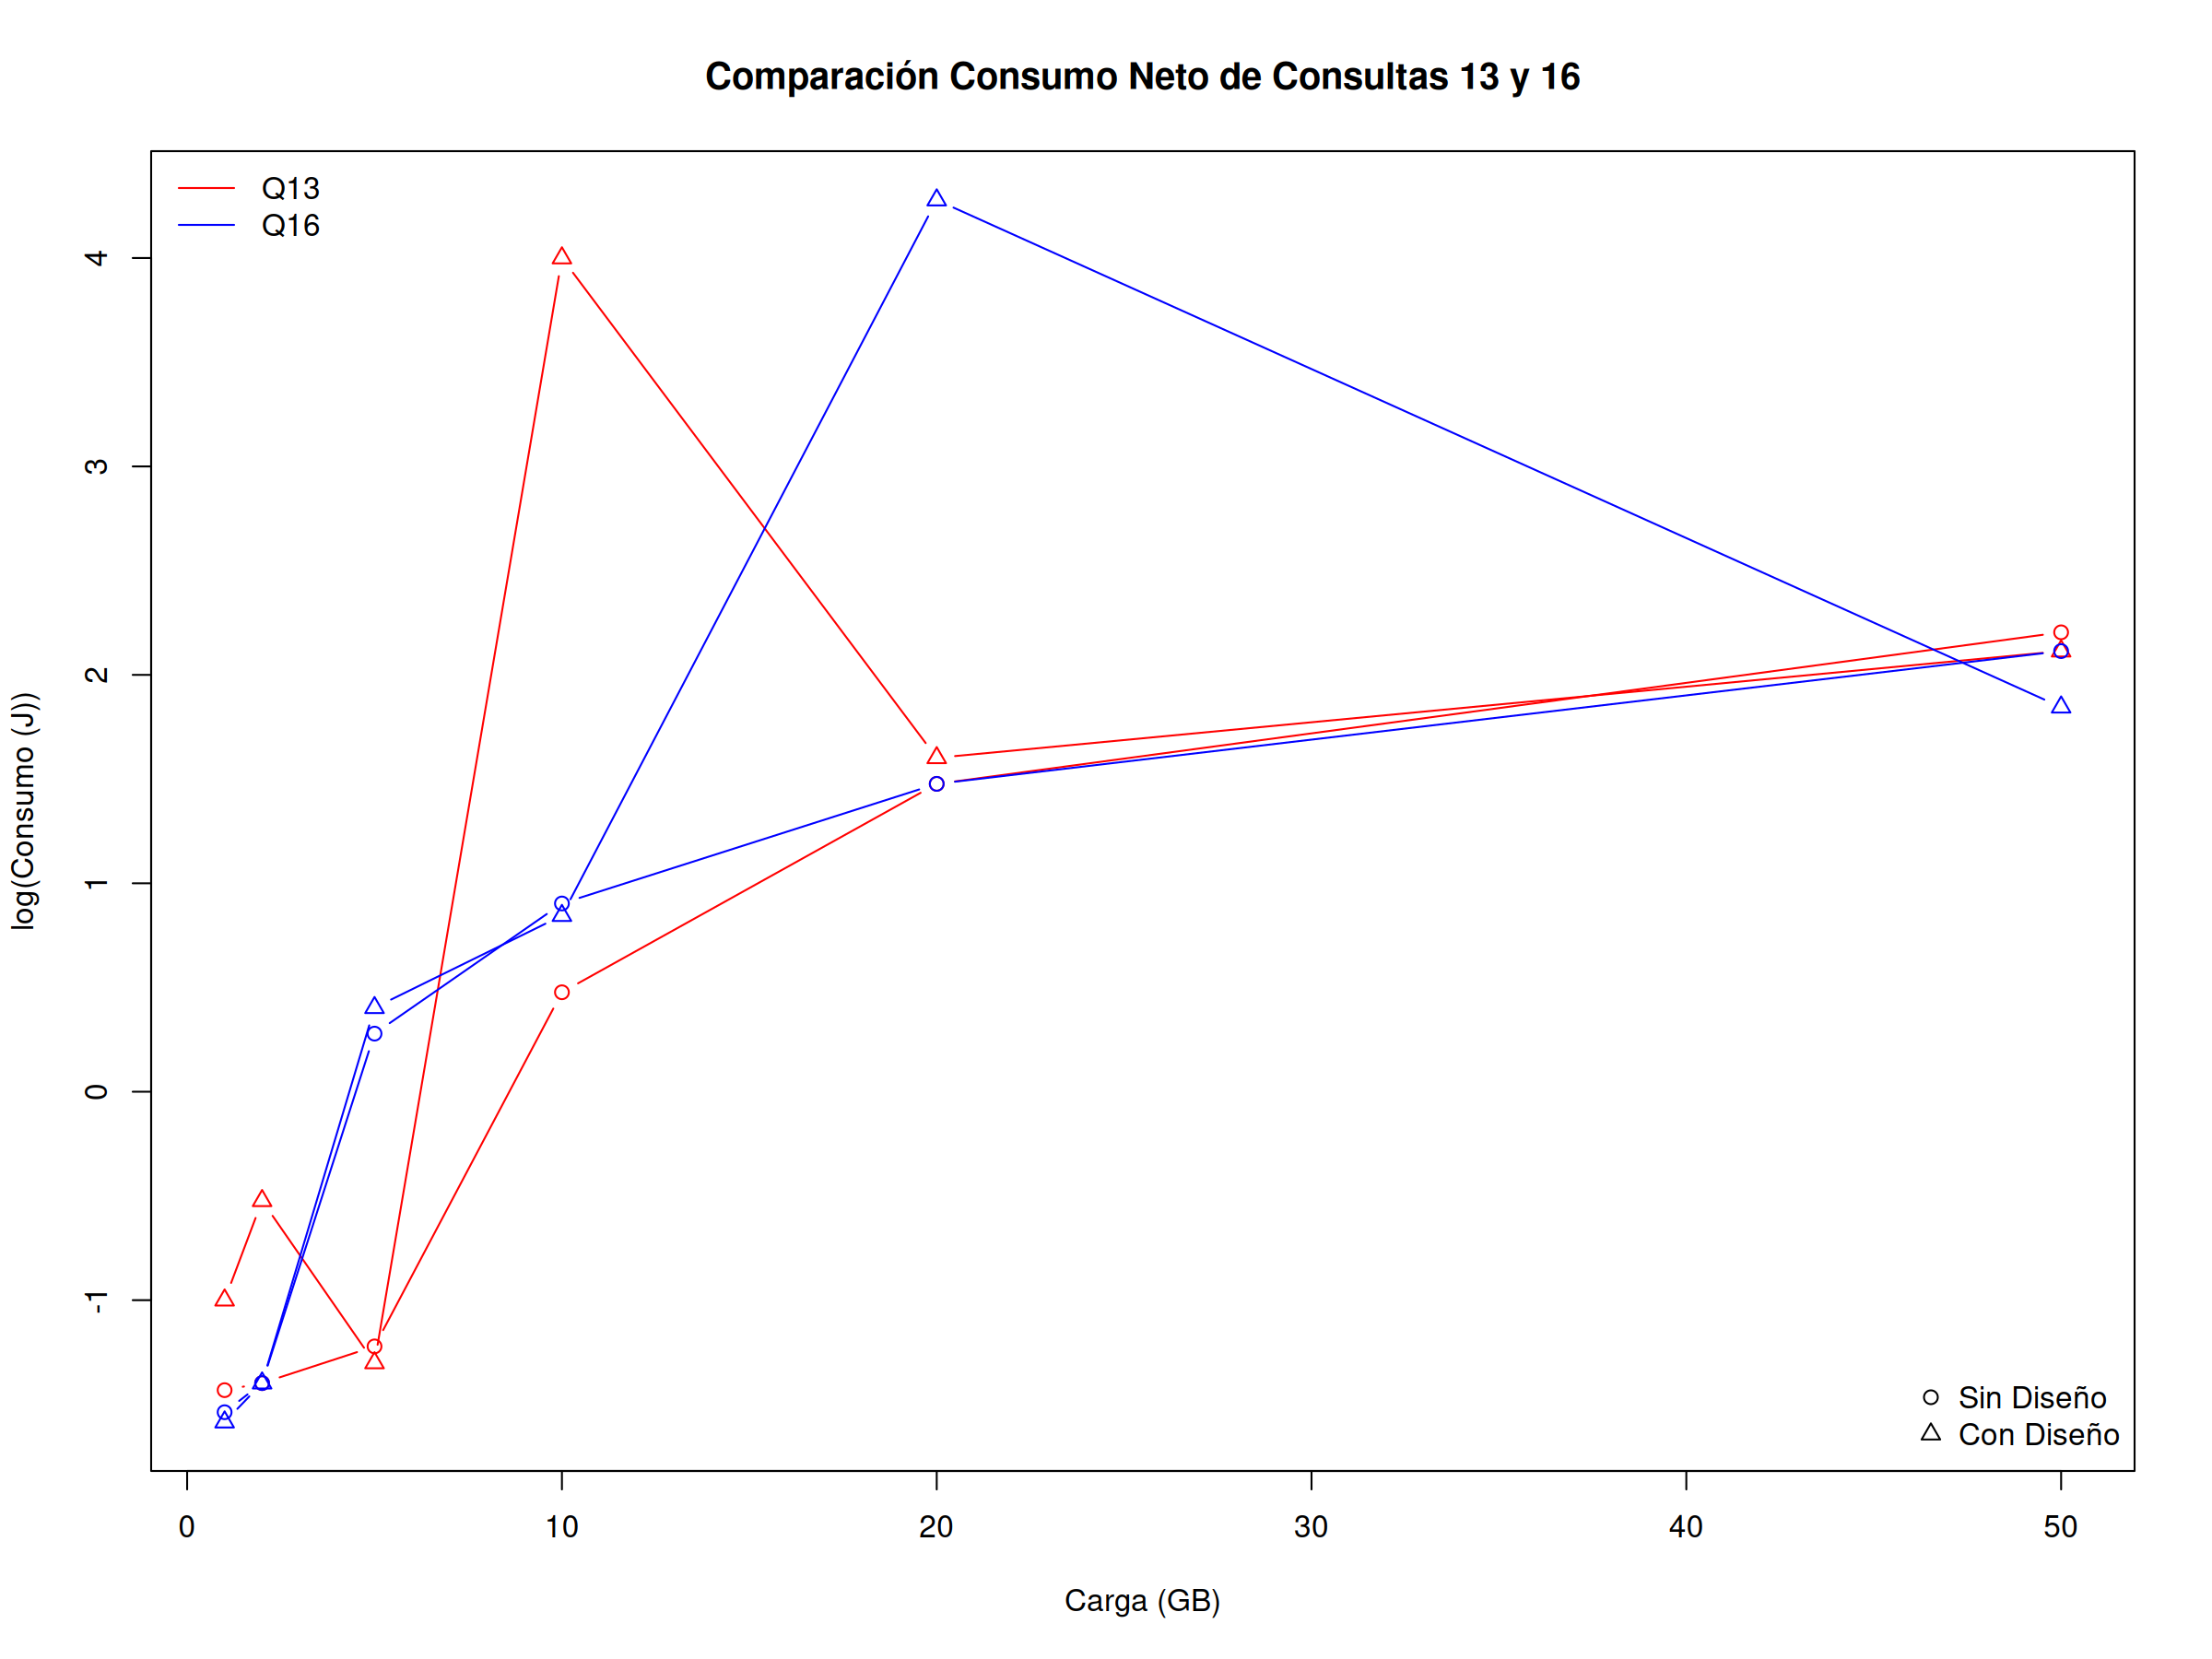
\includegraphics[width = 0.49\textwidth]{images/defensa/cExtremo1.png}
          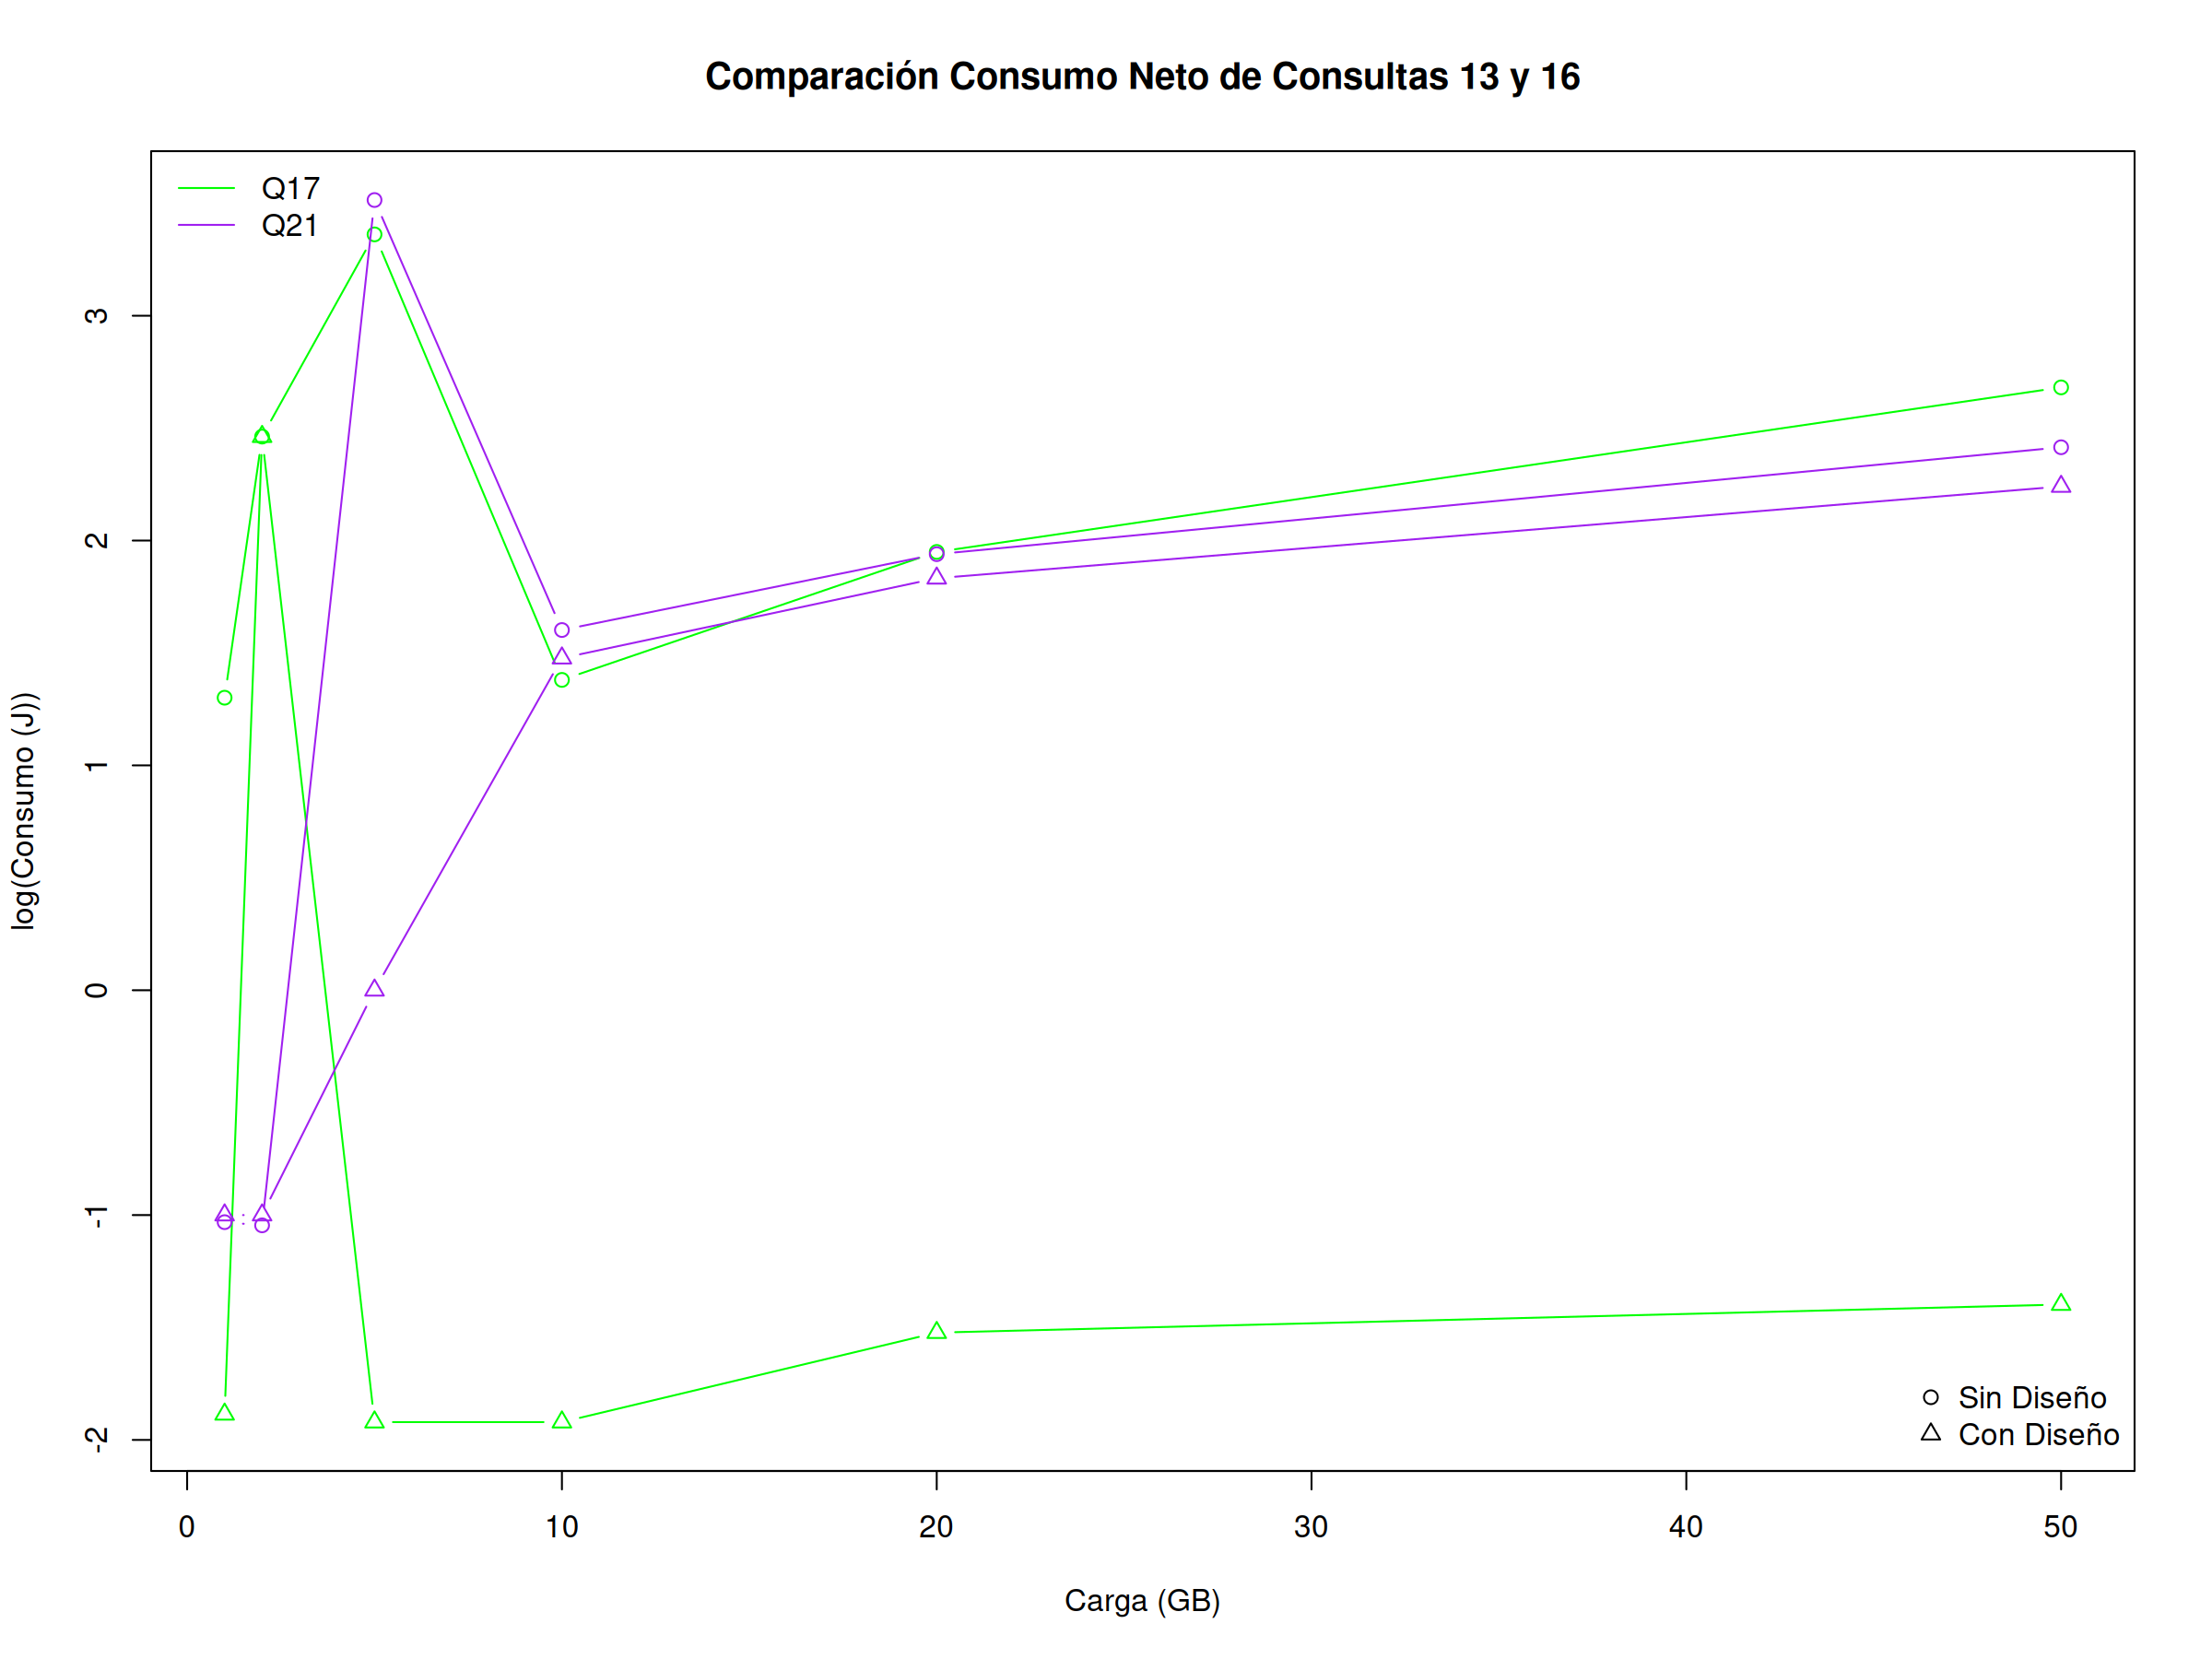
\includegraphics[width = 0.49\textwidth]{images/defensa/cExtremo2.png}
          \caption{Comparación de consultas: consumo neto (extremo)}
        \end{figure}
      \end{frame}

      \begin{frame}{Comparación global por cargas}
        \begin{figure}
          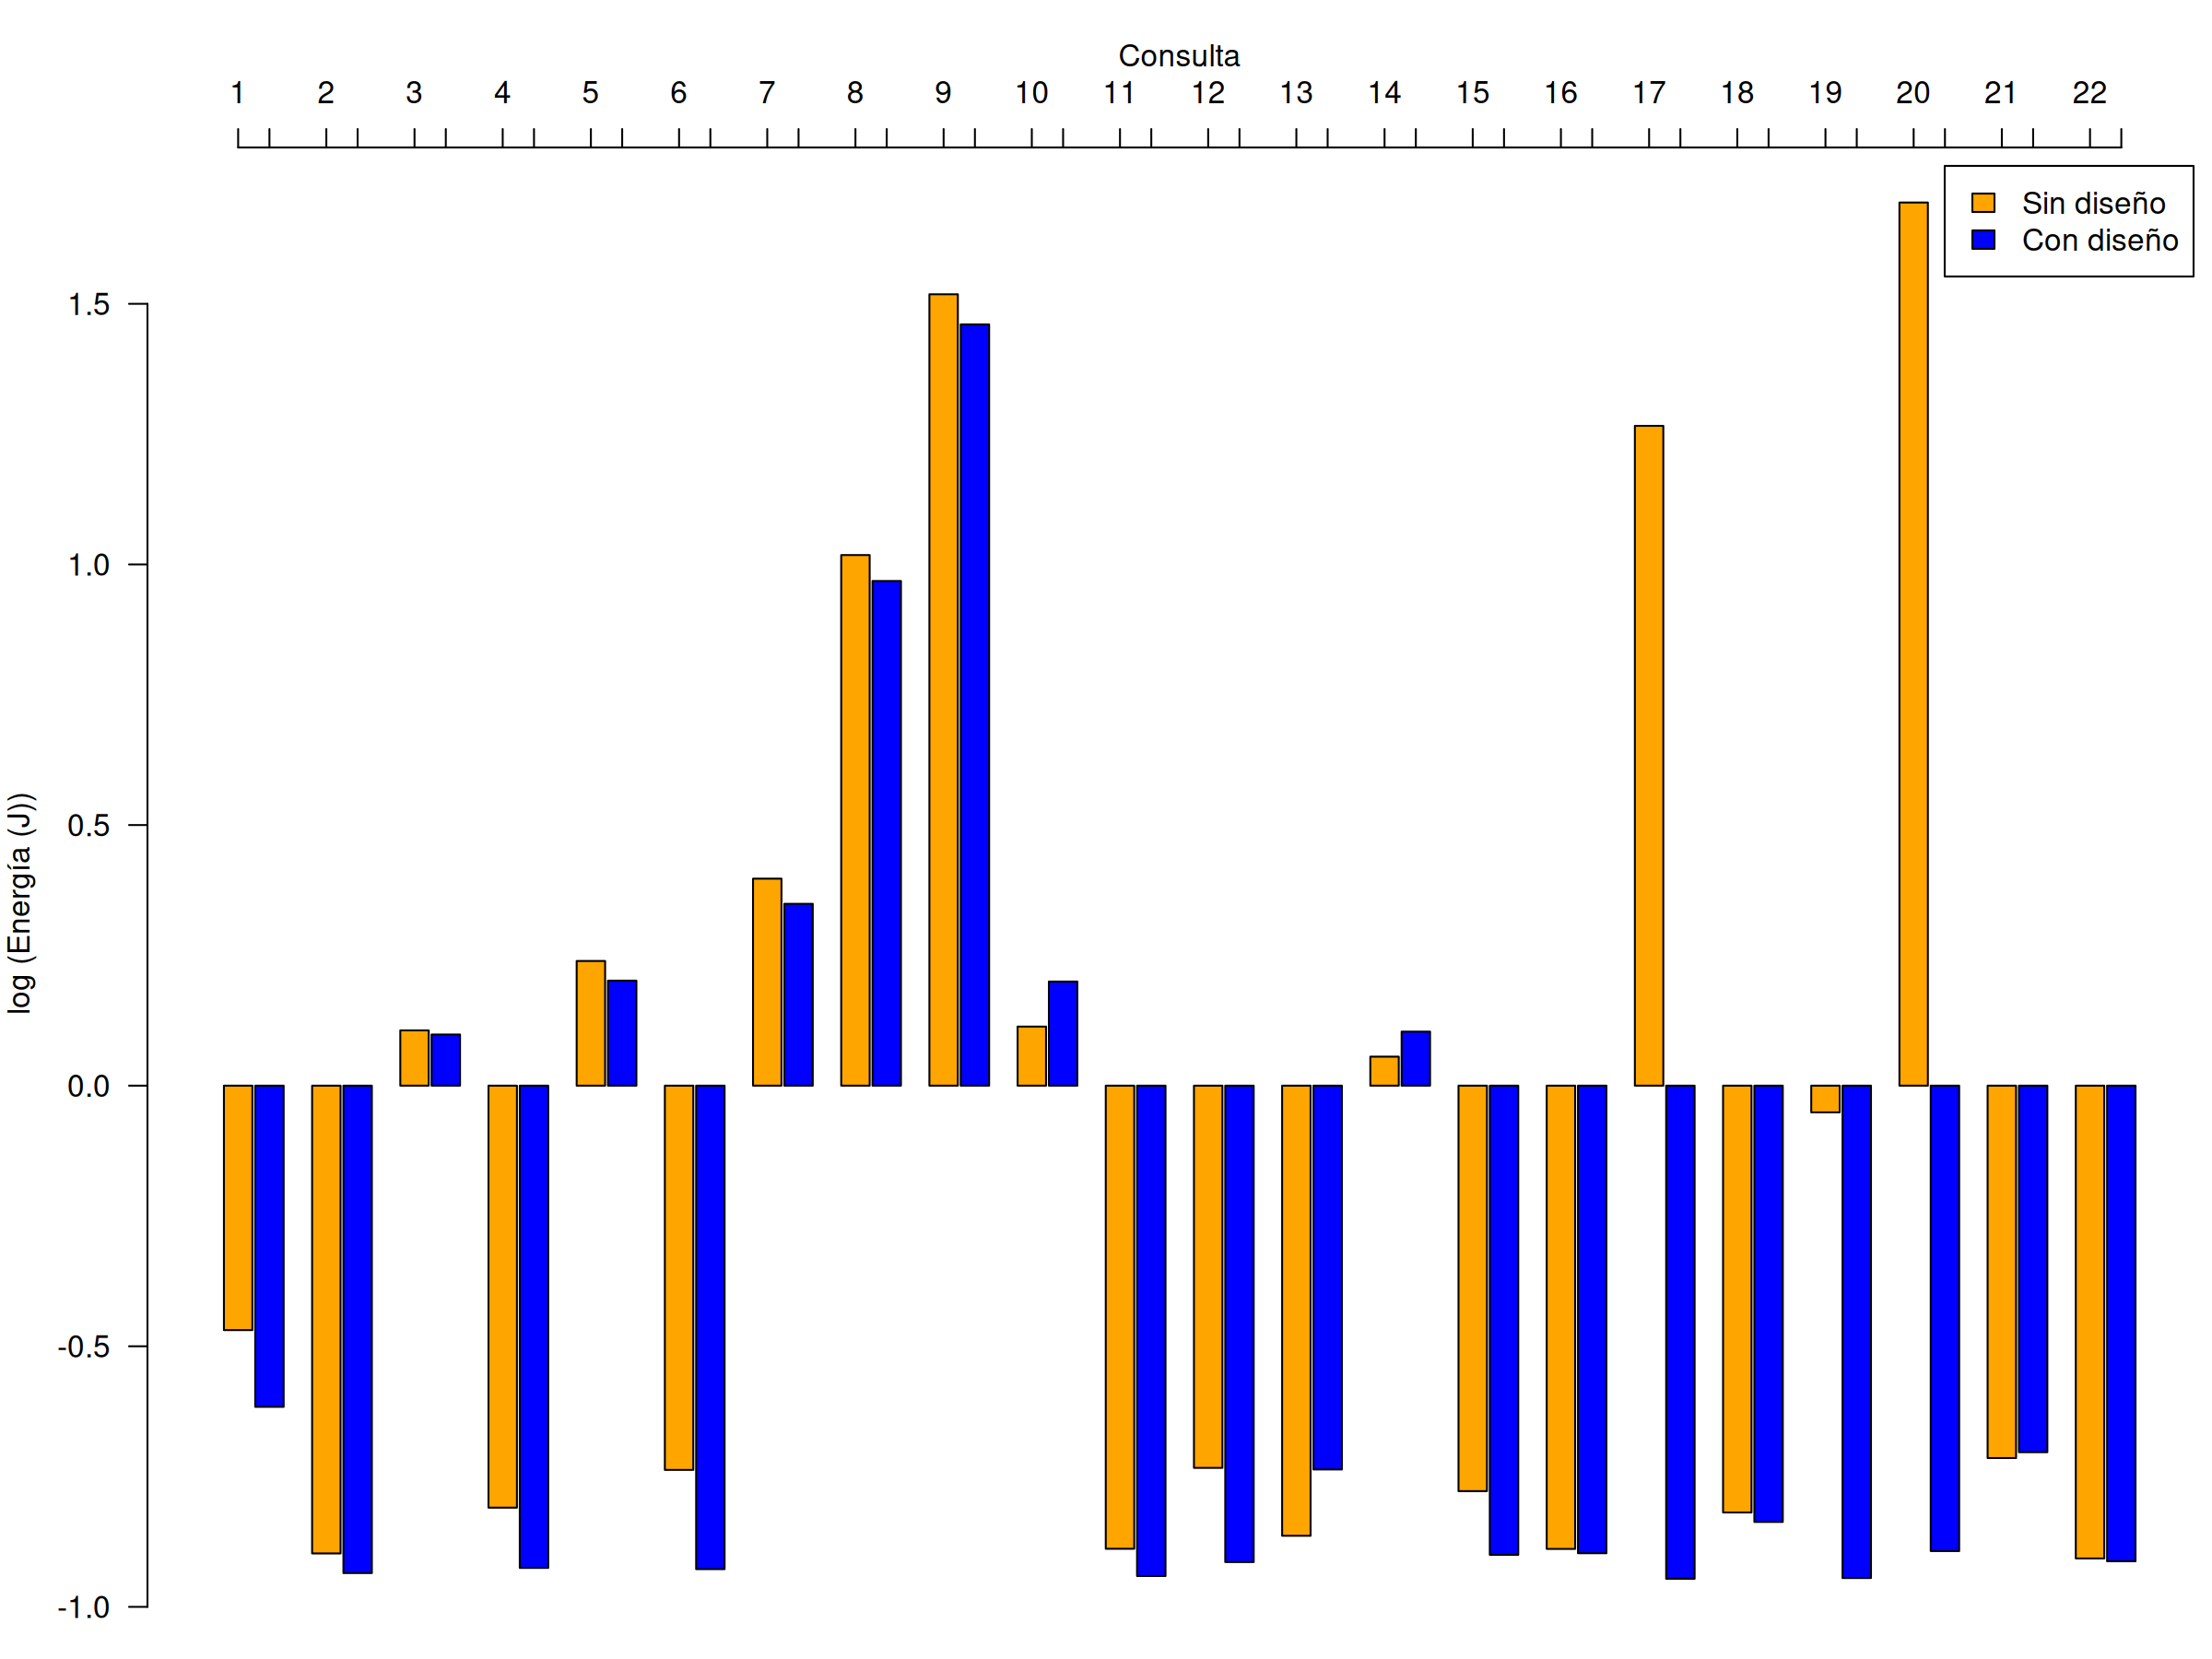
\includegraphics[width = 0.49\textwidth]{images/Neto-1G.png}
          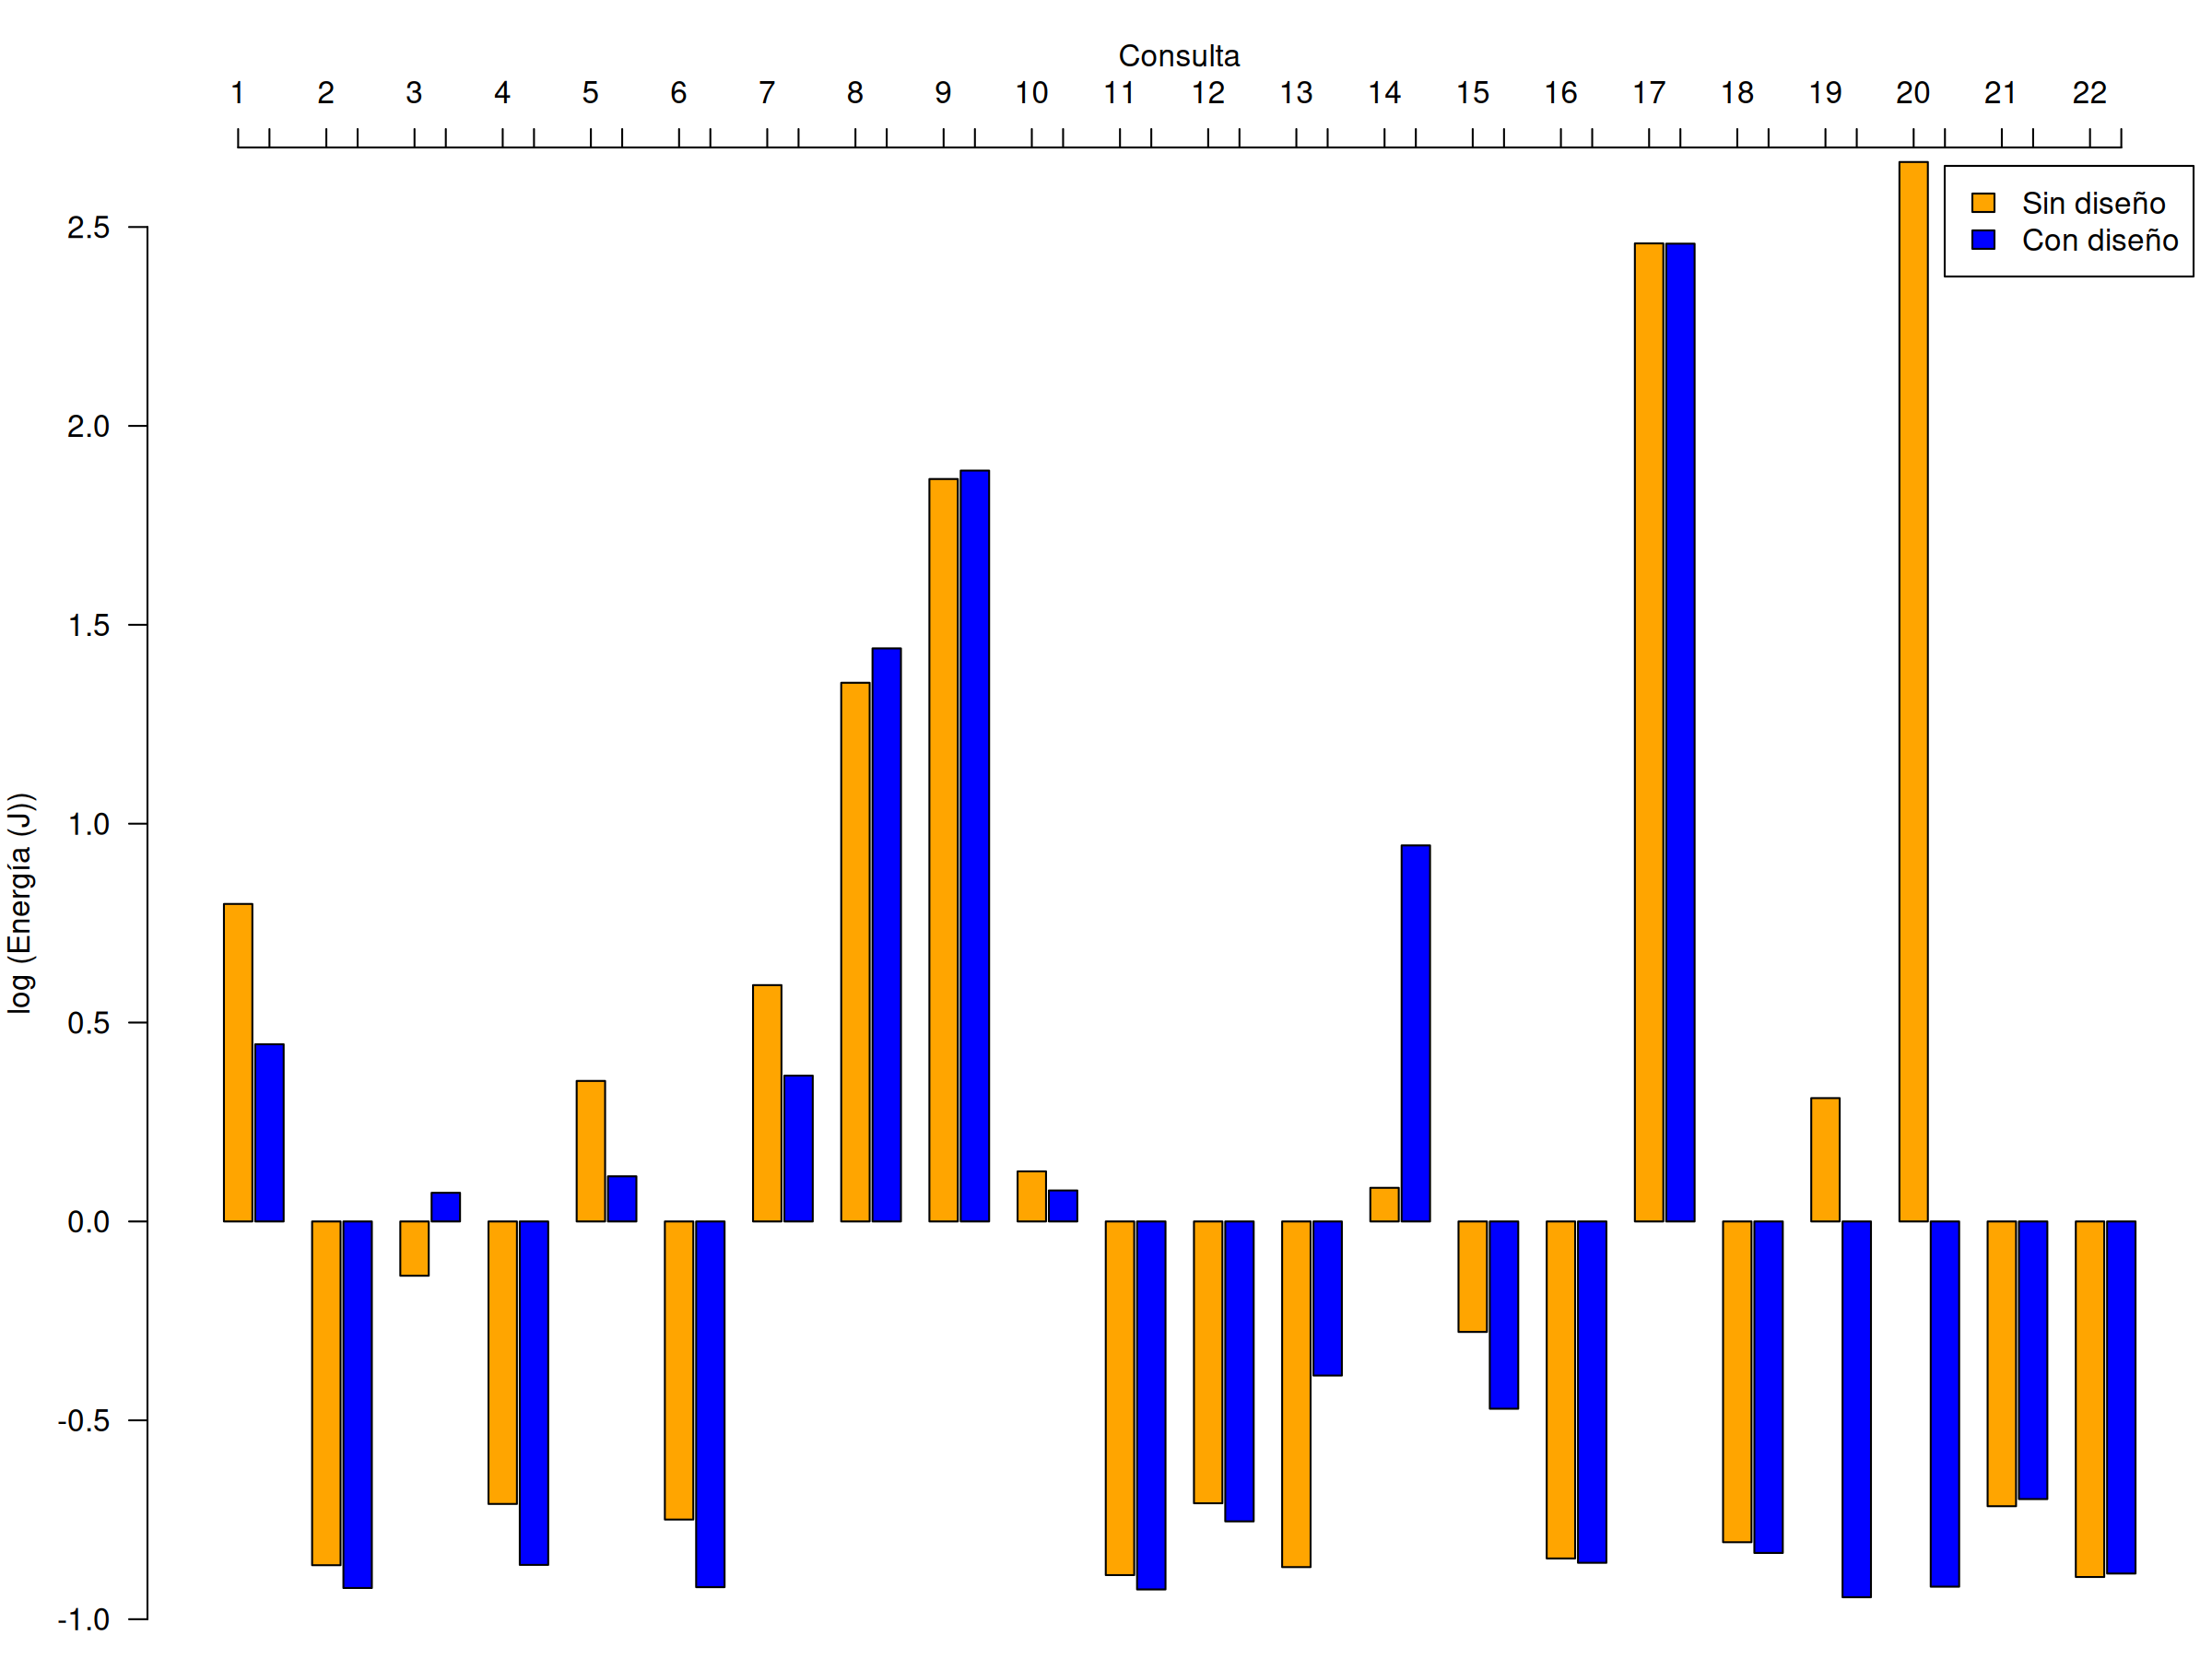
\includegraphics[width = 0.49\textwidth]{images/Neto-2G.png}
          \caption{Consumo neto por consulta 1 GB (izquierda) y 2 GB (derecha)}
        \end{figure}
      \end{frame}

      \begin{frame}{Comparación global por cargas}
        \begin{figure}
          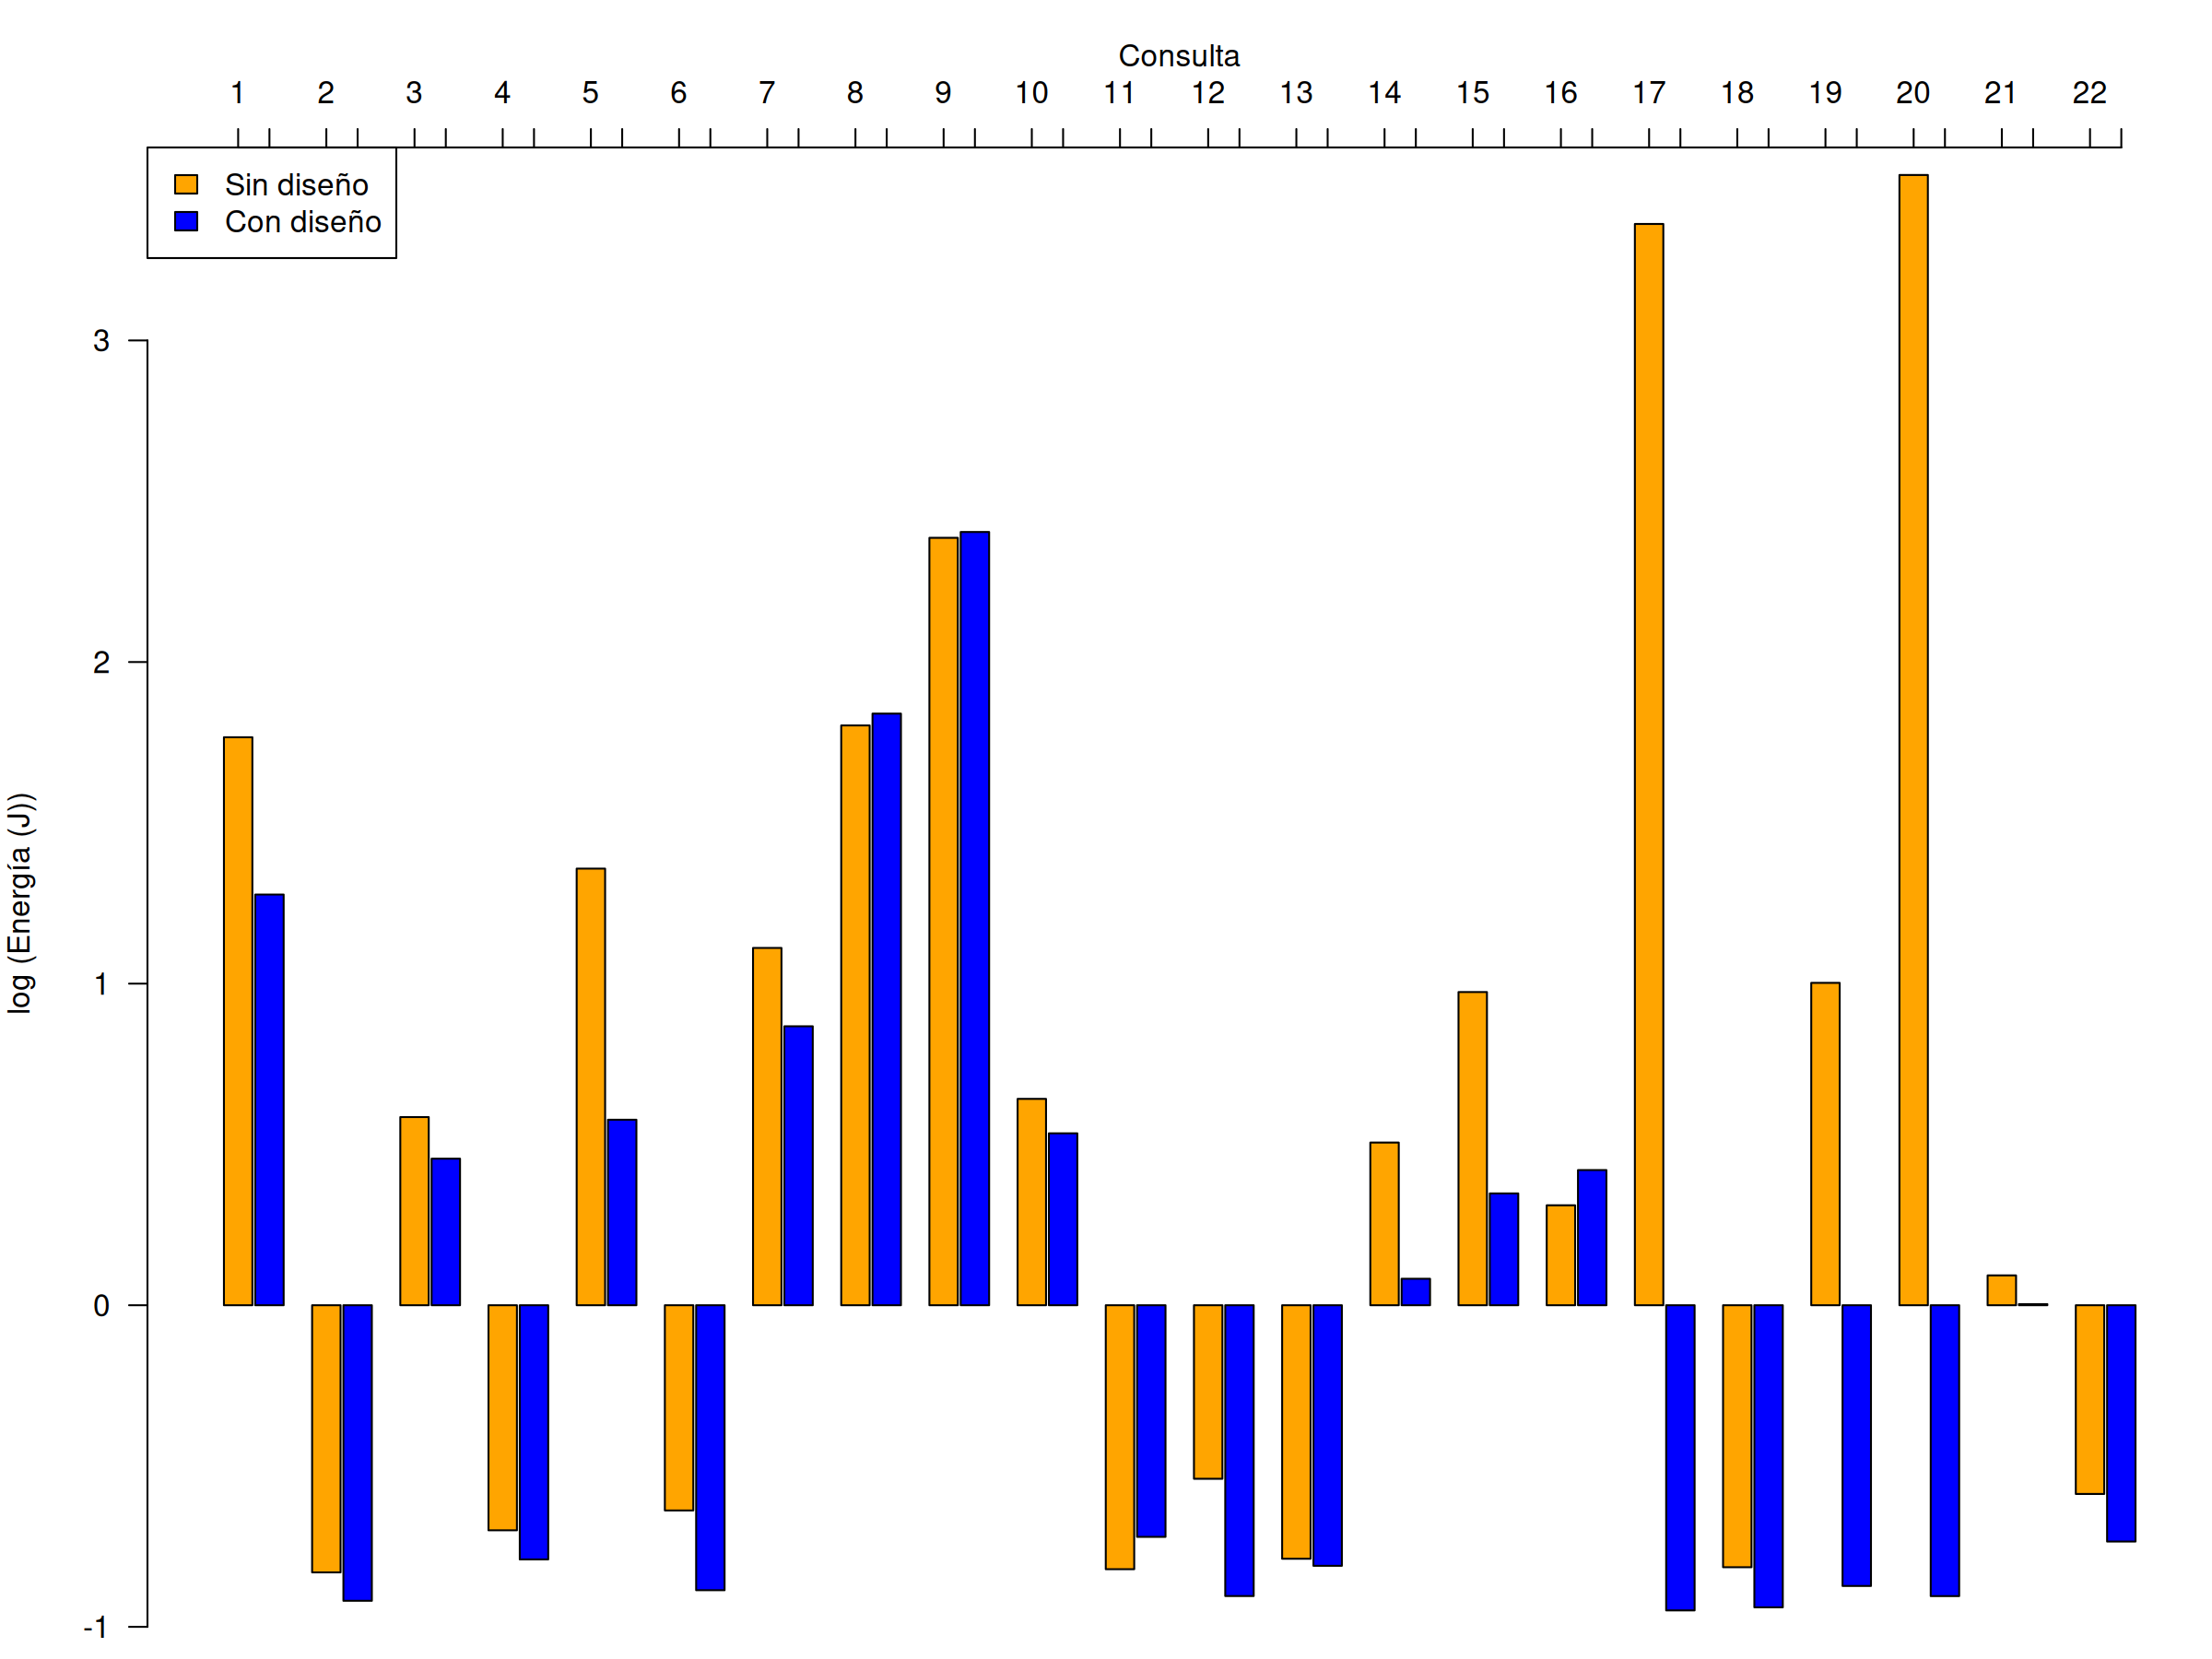
\includegraphics[width = 0.49\textwidth]{images/Neto-5G.png}
          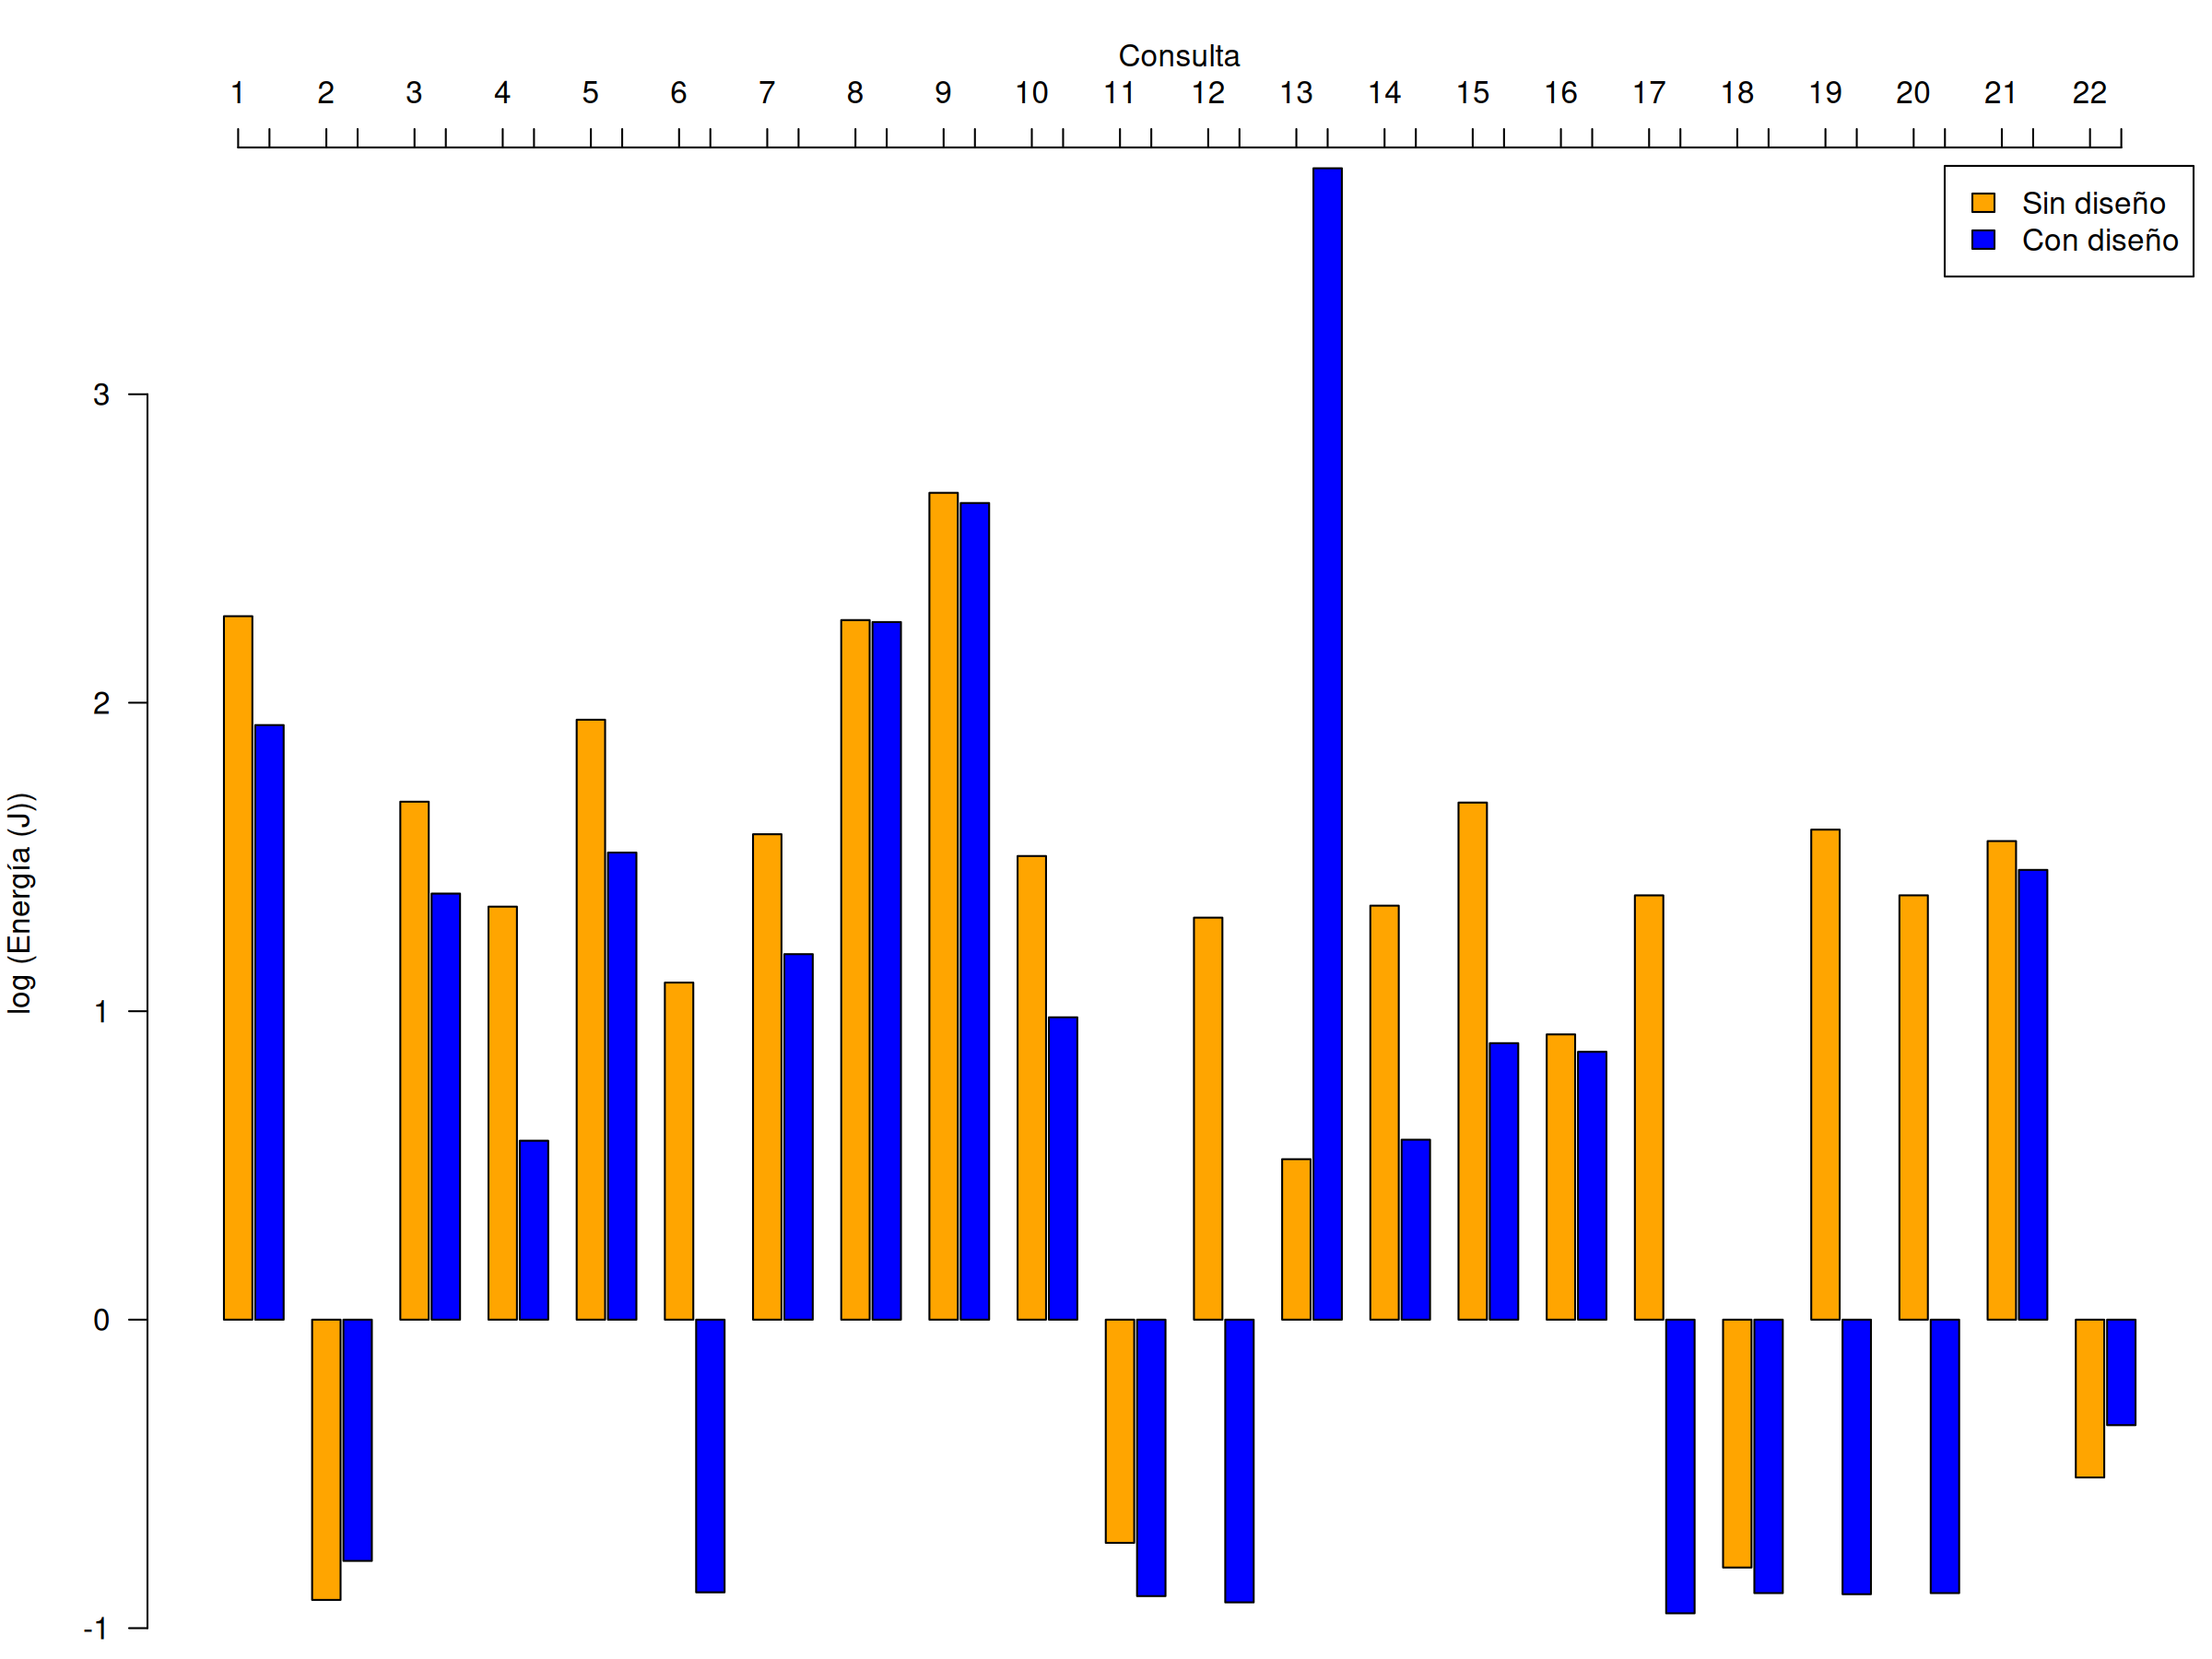
\includegraphics[width = 0.49\textwidth]{images/Neto-10G.png}
          \caption{Consumo neto por consulta 5 GB (izquierda) y 10 GB (derecha)}
        \end{figure}
      \end{frame}

      \begin{frame}{Comparación global por cargas}
        \begin{figure}
          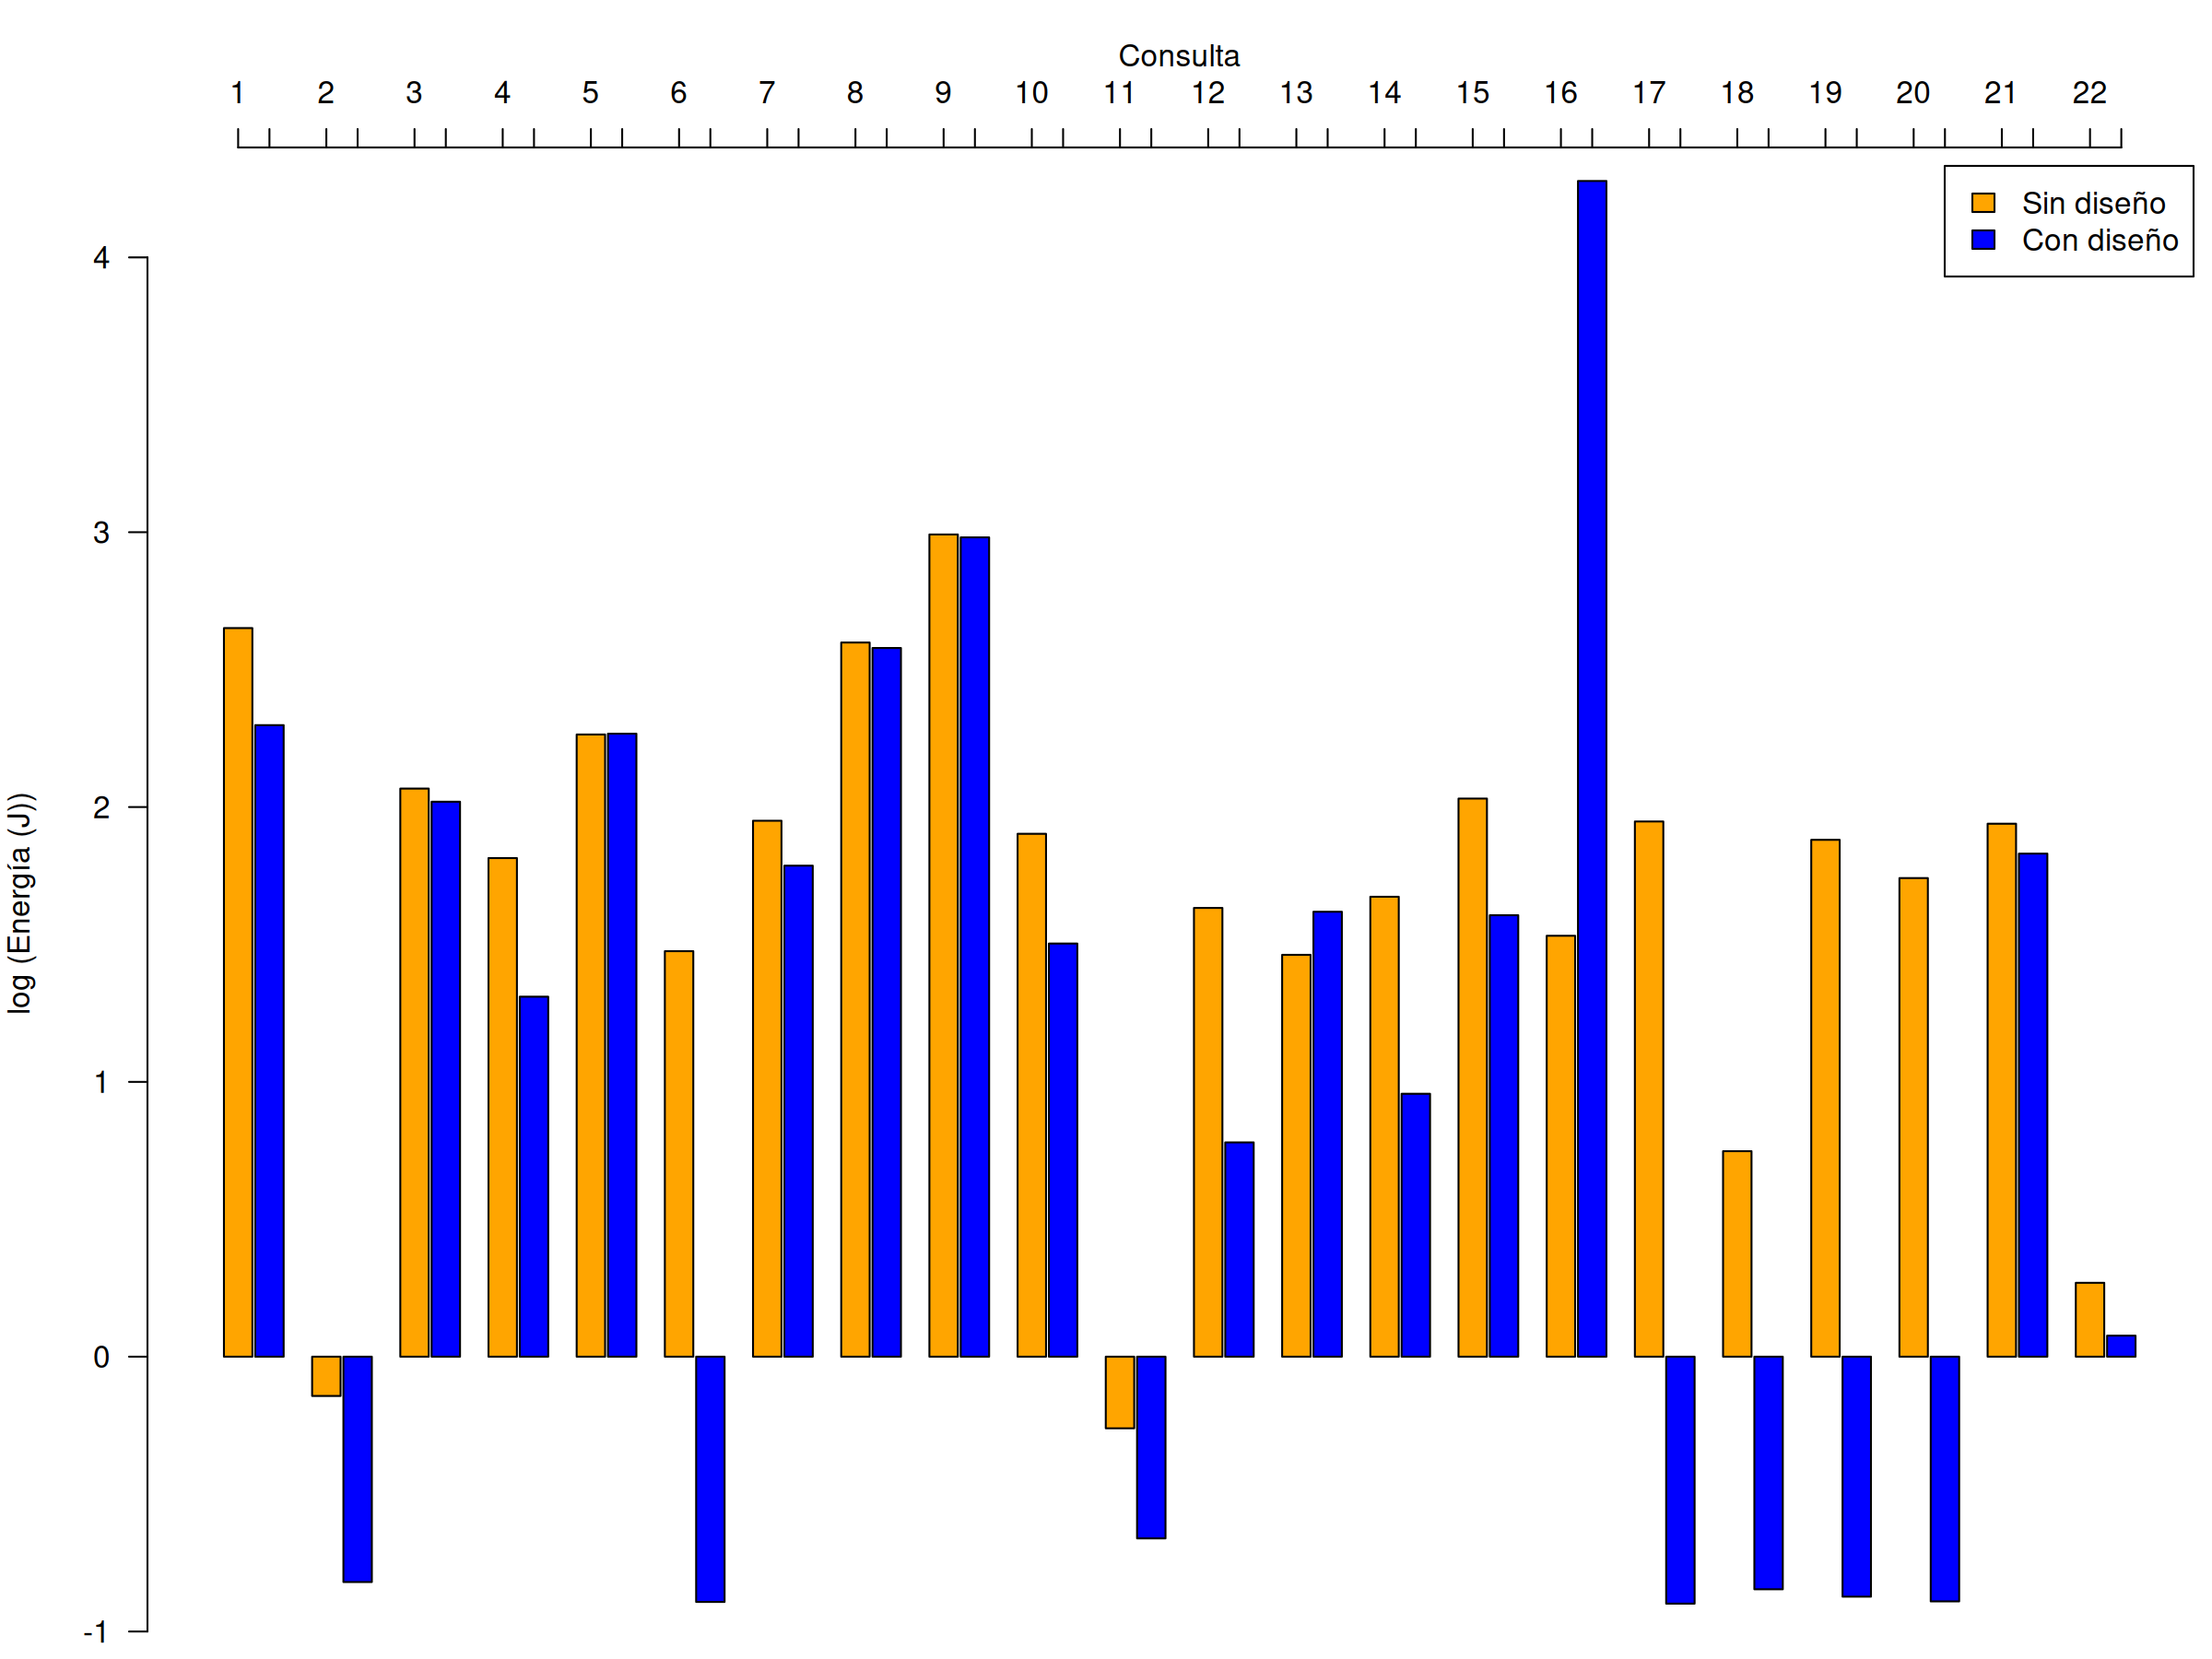
\includegraphics[width = 0.49\textwidth]{images/Neto-20G.png}
          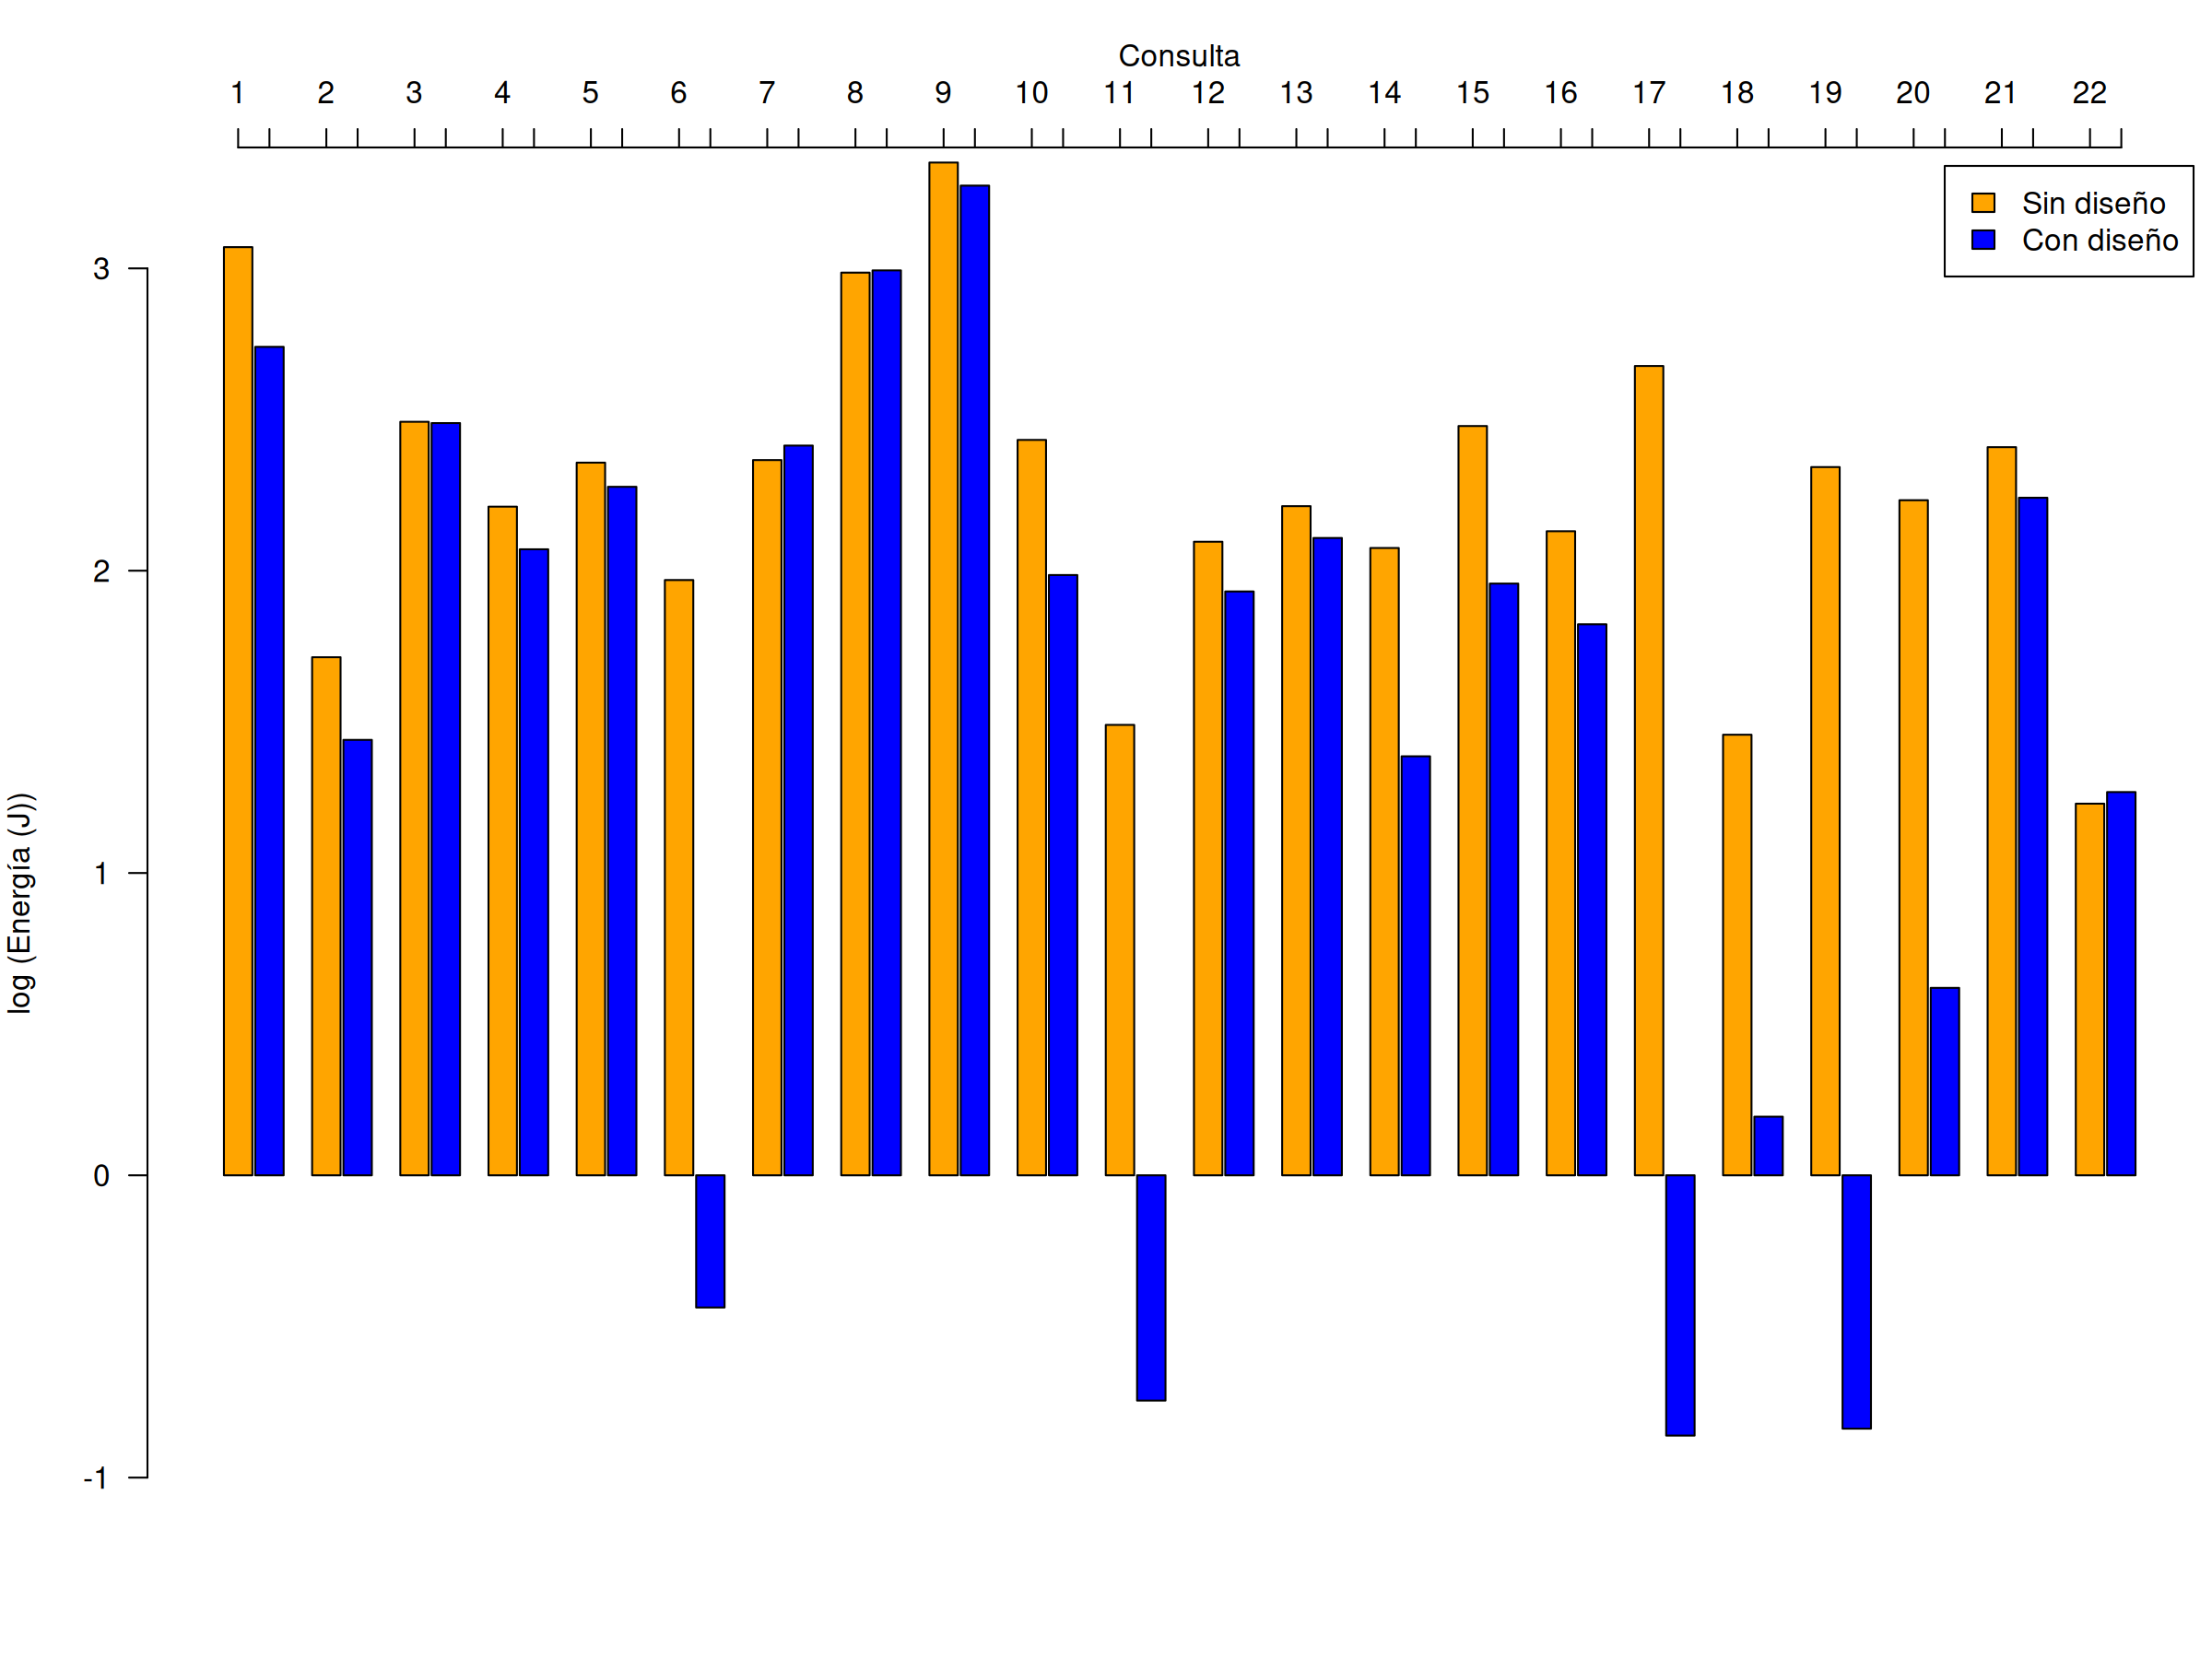
\includegraphics[width = 0.49\textwidth]{images/Neto-50G.png}
          \caption{Consumo neto por consulta 20 GB (izquierda) y 50 GB (derecha)}
        \end{figure}
      \end{frame}
    % subsection consumo_neto (end)

    \subsection{Consumo del coordinador} % (fold)
    \label{sub:consumo_del_coordinador}
      \begin{frame}{Coordinador (con diseño vs Sin diseño)}
        \begin{figure}[H]
          
\includegraphics[width = 0.49\textwidth]{images/Coordinador-1G.png}
          
\includegraphics[width = 0.49\textwidth]{images/Coordinador-2G.png}
          \caption{Consumo coordinador 1 GB (izquierda) y 2 GB (derecha)}
        \end{figure}
      \end{frame}

      \begin{frame}{Coordinador (con diseño vs Sin diseño)}
        \begin{figure}[H]
          
\includegraphics[width = 0.49\textwidth]{images/Coordinador-5G.png}
          
\includegraphics[width = 0.49\textwidth]{images/Coordinador-10G.png}
          \caption{Consumo coordinador 5 GB (izquierda) y 10 GB (derecha)}
        \end{figure}
      \end{frame}

      \begin{frame}{Coordinador (con diseño vs Sin diseño)}
        \begin{figure}[H]
          
\includegraphics[width = 0.49\textwidth]{images/Coordinador-20G.png}
          
\includegraphics[width = 0.49\textwidth]{images/Coordinador-50G.png}
          \caption{Consumo coordinador 20 GB (izquierda) y 50 GB (derecha)}
        \end{figure}
      \end{frame}
    % subsection consumo_del_coordinador (end)

    \subsection{Pruebas estadísticas} % (fold)
    \label{sub:pruebas_estadísticas}
      \begin{frame}{Normalidad}
        \begin{table}[H]
          \centering
          \caption{Prueba de Shapiro-Wilk ($p$-valores)}
          \footnotesize
          \begin{tabular}{| c | c | c | c | c | c |}
            \hline
            Carga (GB) &    Tiempo   & Cons. Coord. & Cons. Trab. 1 & Cons. Trab. 2 & Cons. Neto  \\ \hline
               1 (SD)  & \num{4e-39} & \num{2e-42}  &  \num{3e-41}  &  \num{9e-42}  & \num{2e-40} \\ \hline
               1 (CD)  & \num{2e-40} & \num{5e-43}  &  \num{3e-44}  &  \num{1e-44}  & \num{2e-43} \\ \hline
               2 (SD)  & \num{6e-37} & \num{1e-43}  &  \num{4e-42}  &  \num{3e-42}  & \num{5e-42} \\ \hline
               2 (CD)  & \num{3e-41} & \num{8e-44}  &  \num{1e-43}  &  \num{4e-44}  & \num{2e-43} \\ \hline
               5 (SD)  & \num{1e-38} & \num{5e-43}  &  \num{9e-43}  &  \num{7e-43}  & \num{9e-43} \\ \hline
               5 (CD)  & \num{6e-42} & \num{3e-43}  &  \num{1e-43}  &  \num{1e-43}  & \num{2e-43} \\ \hline
              10 (SD)  & \num{6e-41} & \num{2e-42}  &  \num{8e-37}  &  \num{4e-37}  & \num{8e-38} \\ \hline
              10 (CD)  & \num{6e-43} & \num{4e-49}  &  \num{2e-49}  &  \num{2e-49}  & \num{2e-49} \\ \hline
              20 (SD)  & \num{2e-42} & \num{5e-41}  &  \num{2e-36}  &  \num{3e-36}  & \num{3e-37} \\ \hline
              20 (CD)  & \num{3e-43} & \num{6e-46}  &  \num{6e-38}  &  \num{5e-40}  & \num{2e-45} \\ \hline
              50 (SD)  & \num{2e-42} & \num{2e-38}  &  \num{9e-36}  &  \num{1e-35}  & \num{2e-36} \\ \hline
              50 (CD)  & \num{6e-44} & \num{1e-32}  &  \num{4e-38}  &  \num{2e-37}  & \num{7e-38} \\ \hline
          \end{tabular}
        \end{table}
      \end{frame}

      \begin{frame}{Correlación de Spearman}
        \begin{table}[H]
          \centering
          \caption{Coeficientes de Spearman ($\rho$)}
          \scriptsize
          \begin{tabular}{| c | c | c | c | c |}
            \hline
            Carga (GB) &      $\rho_M(p)$     &      $\rho_1(p)$     &      $\rho_2(p)$     &      $\rho_N(p)$     \\ \hline
               1 (SD)  & 0,8030(0)            & 0,8551(0)            & 0,8723(0)            & 0,9003(0)            \\ \hline
               1 (CD)  & 0,9081(0)            & 0,8721(0)            & 0,8627(0)            & 0,9077(0)            \\ \hline
               2 (SD)  & 0,8068(0)            & 0,8554(0)            & 0,8417(0)            & 0,8807(0)            \\ \hline
               2 (CD)  & 0,8005(0)            & 0,5915(0)            & 0,5758(\num{2e-59})  & 0,6272(0)            \\ \hline
               5 (SD)  & 0,7813(0)            & 0,8865(0)            & 0,8925(0)            & 0,9323(0)            \\ \hline
               5 (CD)  & 0,8219(\num{1e-162}) & 0,8419(\num{3e-178}) & 0,8113(\num{2e-155}) & 0,8756(\num{8e-210}) \\ \hline
              10 (SD)  & 0,7657(\num{3e-128}) & 0,8921(\num{4e-229}) & 0,7857(0)            & 0,8813(0)            \\ \hline
              10 (CD)  & 0,7411(\num{6e-116}) & 0,8631(\num{2e-197}) & 0,8874(\num{2e-223}) & 0,8910(\num{8e-228}) \\ \hline
              20 (SD)  & 0,6980(\num{2e-97})  & 0,8395(\num{2e-176}) & 0,9030(\num{1e-243}) & 0,9024(\num{1e-242}) \\ \hline
              20 (CD)  & 0,7260(\num{4e-109}) & 0,8806(\num{1e-215}) & 0,8612(\num{1e-195}) & 0,8618(\num{4e-196}) \\ \hline
              50 (SD)  & 0,7579(0)            & 0,8539(0)            & 0,8503(0)            & 0,8805(0)            \\ \hline
              50 (CD)  & 0,7726(\num{6e-132}) & 0,8887(\num{5e-225}) & 0,9033(\num{5e-244}) & 0,9267(\num{6e-282}) \\ \hline
          \end{tabular}
        \end{table}
      \end{frame}

      \begin{frame}{Correlación de Kendall}
        \begin{table}[H]
          \centering
          \caption{Coeficientes de Kendall ($\tau$)}
          \scriptsize
          \begin{tabular}{| c | c | c | c | c |}
            \hline
            Carga (GB) &      $\tau_M(p)$     &      $\tau_1(p)$     &      $\tau_2(p)$     &      $\tau_N(p)$     \\ \hline
               1 (SD)  & 0,6222(\num{2e-126}) & 0,6603(\num{4e-142}) & 0,6720(\num{4e-147}) & 0,7117(\num{1e-164}) \\ \hline
               1 (CD)  & 0,7425(\num{4e-179}) & 0,6922(\num{6e-156}) & 0,6916(\num{1e-155}) & 0,7439(\num{8e-180}) \\ \hline
               2 (SD)  & 0,6244(\num{3e-127}) & 0,6612(\num{2e-142}) & 0,6423(\num{1e-134}) & 0,6918(\num{1e-155}) \\ \hline
               2 (CD)  & 0,6424(\num{1e-134}) & 0,4953(\num{9e-81})  & 0,4737(\num{5e-74})  & 0,5367(\num{2e-94})  \\ \hline
               5 (SD)  & 0,5783(\num{2e-109}) & 0,7144(\num{6e-166}) & 0,7244(\num{1e-170}) & 0,7812(\num{5e-198}) \\ \hline
               5 (CD)  & 0,6204(\num{2e-125}) & 0,6495(\num{2e-137}) & 0,6149(\num{3e-123}) & 0,6880(\num{7e-154}) \\ \hline
              10 (SD)  & 0,6020(\num{2e-118}) & 0,7239(\num{2e-170}) & 0,6047(\num{2e-119}) & 0,7090(\num{2e-163}) \\ \hline
              10 (CD)  & 0,5214(\num{2e-89})  & 0,6706(\num{2e-146}) & 0,6955(\num{2e-157}) & 0,7037(\num{4e-161}) \\ \hline
              20 (SD)  & 0,5181(\num{3e-88})  & 0,6536(\num{3e-139}) & 0,7344(\num{3e-175}) & 0,7296(\num{5e-173}) \\ \hline
              20 (CD)  & 0,5148(\num{4e-87})  & 0,6910(\num{2e-155}) & 0,6612(\num{2e-142}) & 0,6707(\num{2e-146}) \\ \hline
              50 (SD)  & 0,5886(\num{3e-113}) & 0,6811(\num{5e-151}) & 0,6782(\num{9e-159}) & 0,7197(\num{2e-168}) \\ \hline
              50 (CD)  & 0,5700(\num{2e-106}) & 0,7082(\num{5e-163}) & 0,7276(\num{5e-172}) & 0,7659(\num{2e-190}) \\ \hline
          \end{tabular}
        \end{table}
      \end{frame}
    % subsection pruebas_estadísticas (end)
  % section resultados (end)

  \section{Conclusiones y recomendaciones} % (fold)
  \label{sec:conclusiones_y_recomendaciones}
    \begin{frame}{Conclusiones}
      \begin{itemize}
        \item Racionalidad en el diseño $\equiv$ Optimización de las variables.
        \item $\{\rho, \tau\} \vdash U \propto t$
        \item La calidad de la optimización depende fuertemente del tamaño del
        clúster.
        \item La optimización traslada parte del consumo energético a la lectura
        y escritura del disco cuando se usan estructuras adicionales dentro de
        las consultas.
        \item La co-locación es crítica para optimizar rendimiento y consumo.
      \end{itemize}
    \end{frame}

    \begin{frame}{Recomendaciones}
      \begin{itemize}
        \item Simular co-locación con atributos sintéticos o con reescritura con
        réplicas de tablas y \texttt{JOIN}.
        \item Estudiar distintas herramientas de medición de alta frecuencia
        para garantizar la correcta medición del consumo en consultas
        optimizadas para ejecutarse en fracciones de segundo.
      \end{itemize}
    \end{frame}
  % section conclusiones_y_recomendaciones (end)

  \begin{frame}[allowframebreaks]{Referencias}
    \small
    \bibliographystyle{IEEEtran}
    \bibliography{Refs}
  \end{frame}
\end{document}